\documentclass{article}

\usepackage{packages}
\usepackage{environments}
\usepackage{commands}

\begin{document}

\title{Algebra\\Lecture Notes}
\author{Dima Trushin}
\date{2023}
	
\maketitle
\tableofcontents

\ProvidesFile{lecture01.tex}[Lecture 1]


\newpage

\section{Sets}

In modern math everything can be formulated in terms of Set Theory, that is in terms of sets and maps.
Let me remind some basic facts about sets and maps.

\subsection{Definition}

\begin{definition}
A set is a collection of elements.
\end{definition}

We denote sets by capital letters like $X$ and $Y$.
If an element $x$ belongs to the collection $X$, we write $x\in X$.
If $y$ does not belong to $X$, we write $y\notin X$.
There is a special set containing no elements.
This set is called an empty set and is denoted by $\varnothing$.

If you think of a set you should imagine a sack full of elements.
The sack is your set and the elements in the sack are the elements belonging to the set.
An empty set becomes a sack with no elements inside.

\subsection{Constructors}

If you are given a definition of a new math object, the first question to ask is: ``How do I construct such an object?'' To define a set we need to specify the elements inside the set.
For doing that, we use the following notation
\[
X = \{x\mid \text{\textbf{condition} on }x\}
\]
Here, we mean that the set $X$ consists of all elements $x$ such that the \textbf{condition} on $x$ holds.
Let me demonstrate this on examples.
\begin{itemize}
\item The set of natural numbers
\[
\mathbb N = \{x\mid x \text{ is a natural number}\} = \{0, 1, 2, 3, \ldots, n,\ldots\}
\]

\item The set of integer numbers
\[
\mathbb Z = \{x\mid x \text{ is an integer number}\} = \{\ldots,-2,-1,0,1,2,\ldots\}
\]

\item The set of real numbers
\[
\mathbb R = \{x\mid x \text{ is a real number}\}
\]
We think of the real numbers as a line containing all possible numbers we use in our calculations.

\item The closed interval $[0, 1]$
\[
[0, 1] = \{x\in \mathbb R \mid 0\leqslant x \leqslant 1\}
\]
Here, I use a slightly different notation.
I specified that $x\in \mathbb R$ before $|$, this simply means that $x$ must be a real number and the additional condition (the number is between zero and one) is written after $|$.

\end{itemize}


\subsection{Operations on sets}

There are several useful procedures you can apply to sets in order to construct new sets.
Let us discuss them.

\subsubsection{Intersection}

If we are given two sets $X$ and $Y$, then we define the intersection of $X$ and $Y$ as follows
\[
X \cap Y = \{z\mid z\in X\text{ and } z\in Y\}
\]
If we denote the sets $X$ and $Y$ by discs on a plain then the intersection of $X$ and $Y$ is denoted as below
\begin{center}
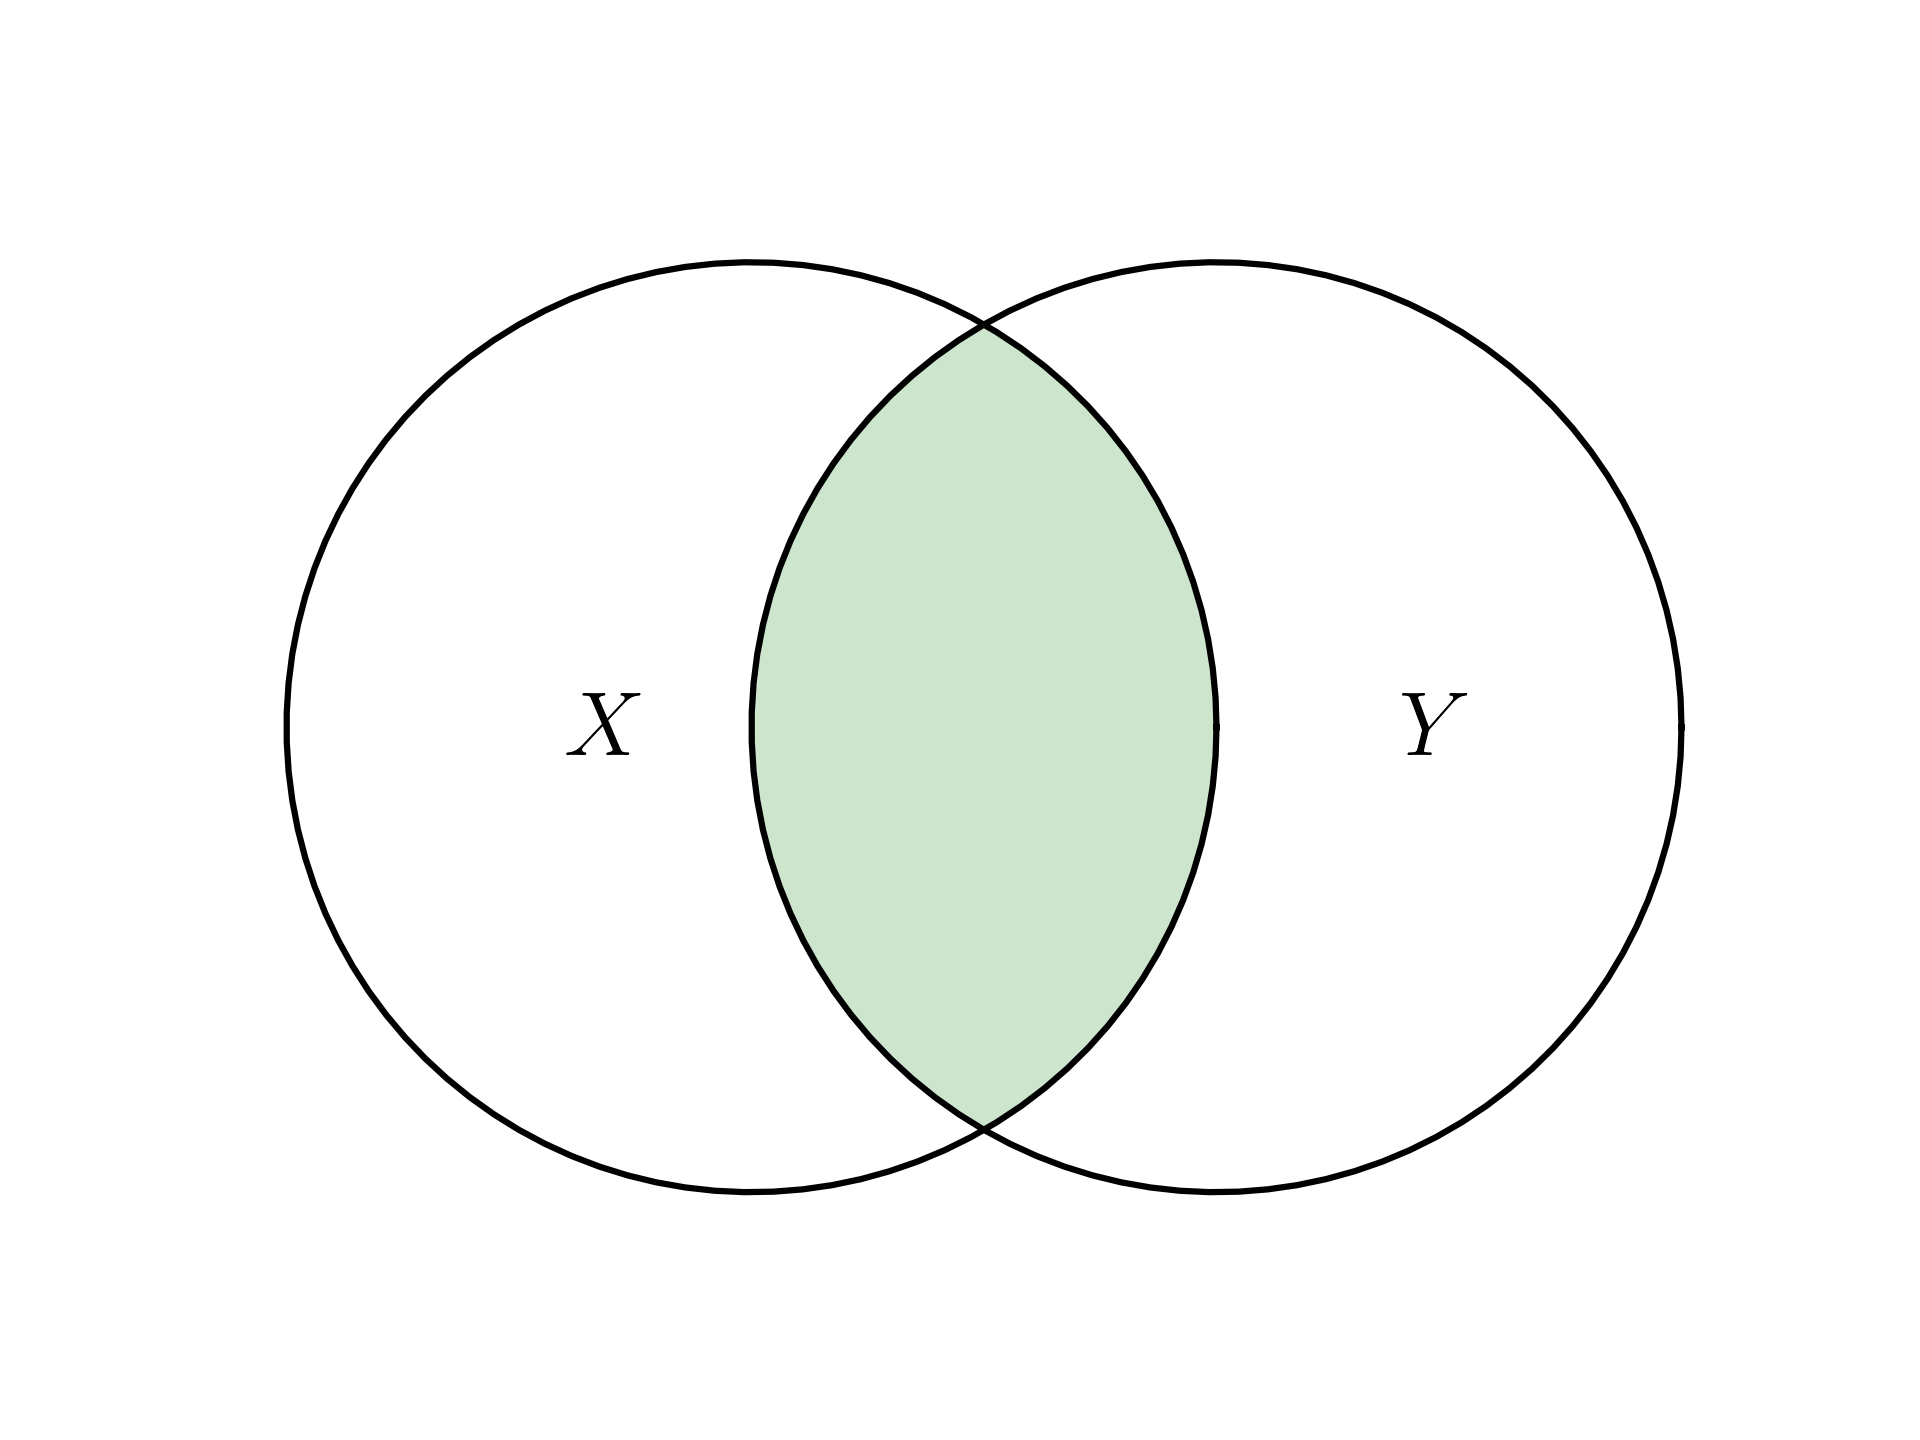
\includegraphics[scale = 0.3]{Figures/graph_intersection.png}
\end{center}

\subsubsection{Union}

If we are given two sets $X$ and $Y$, then we define the union of $X$ and $Y$ as follows
\[
X \cup Y = \{z\mid z\in X\text{ or }z\in Y\}
\]
If we denote the sets $X$ and $Y$ by discs on a plain then the union of $X$ and $Y$ is denoted as below
\begin{center}
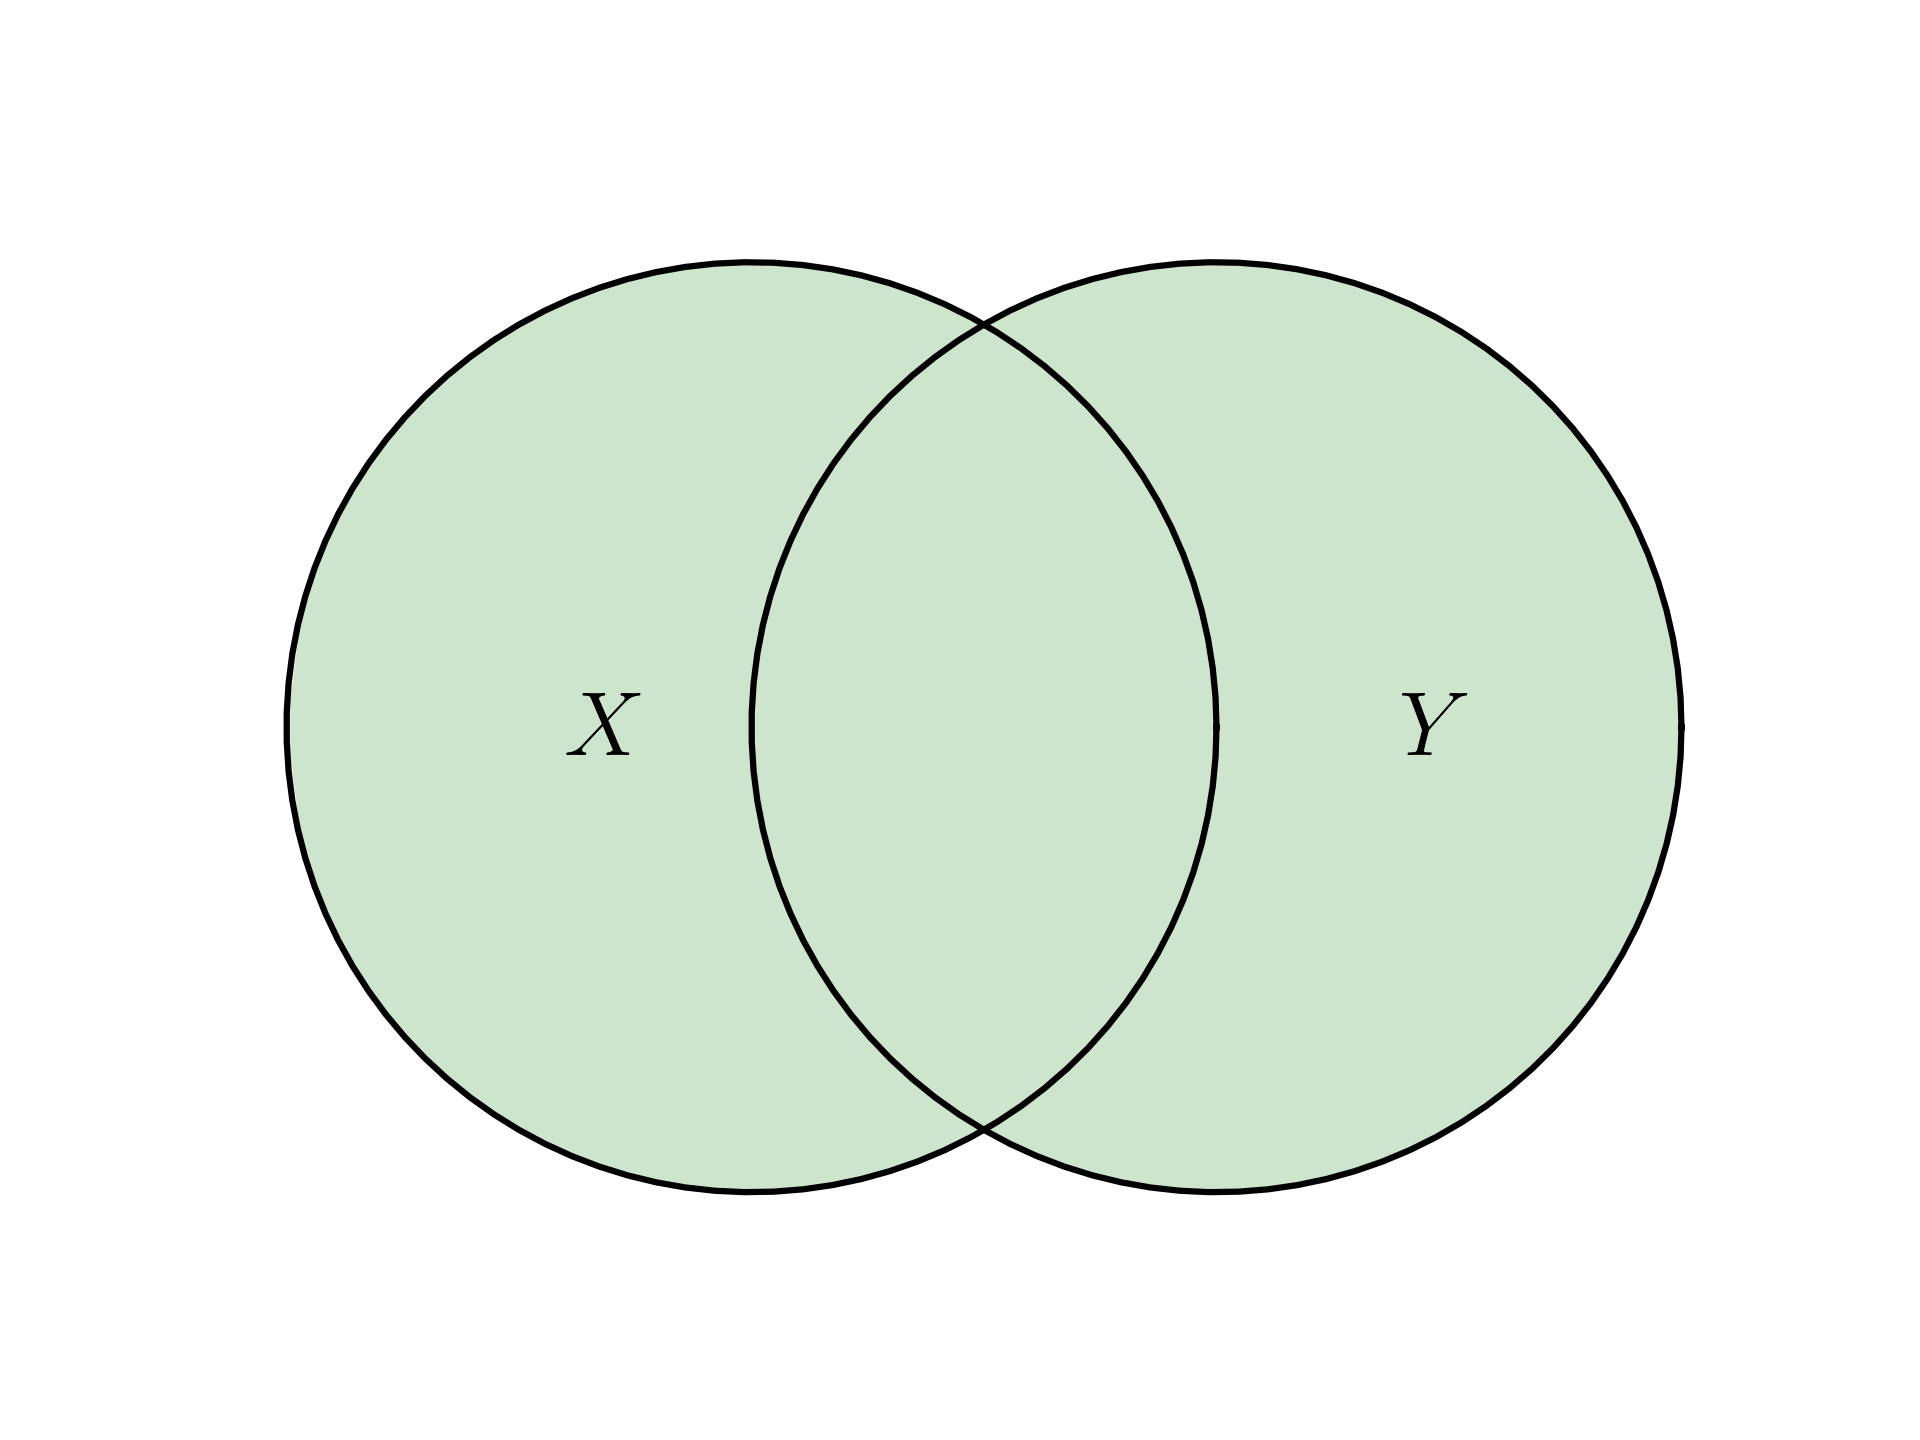
\includegraphics[scale = 0.3]{Figures/graph_union.png}
\end{center}

\subsubsection{Difference}

If we are given two sets $X$ and $Y$, then we define the difference between $X$ and $Y$ as follows
\[
X\setminus Y = \{z\mid z\in X\text{ and }z\notin Y\}
\]
If we denote the sets $X$ and $Y$ by discs on a plain then the difference between $X$ and $Y$ is denoted as below
\begin{center}
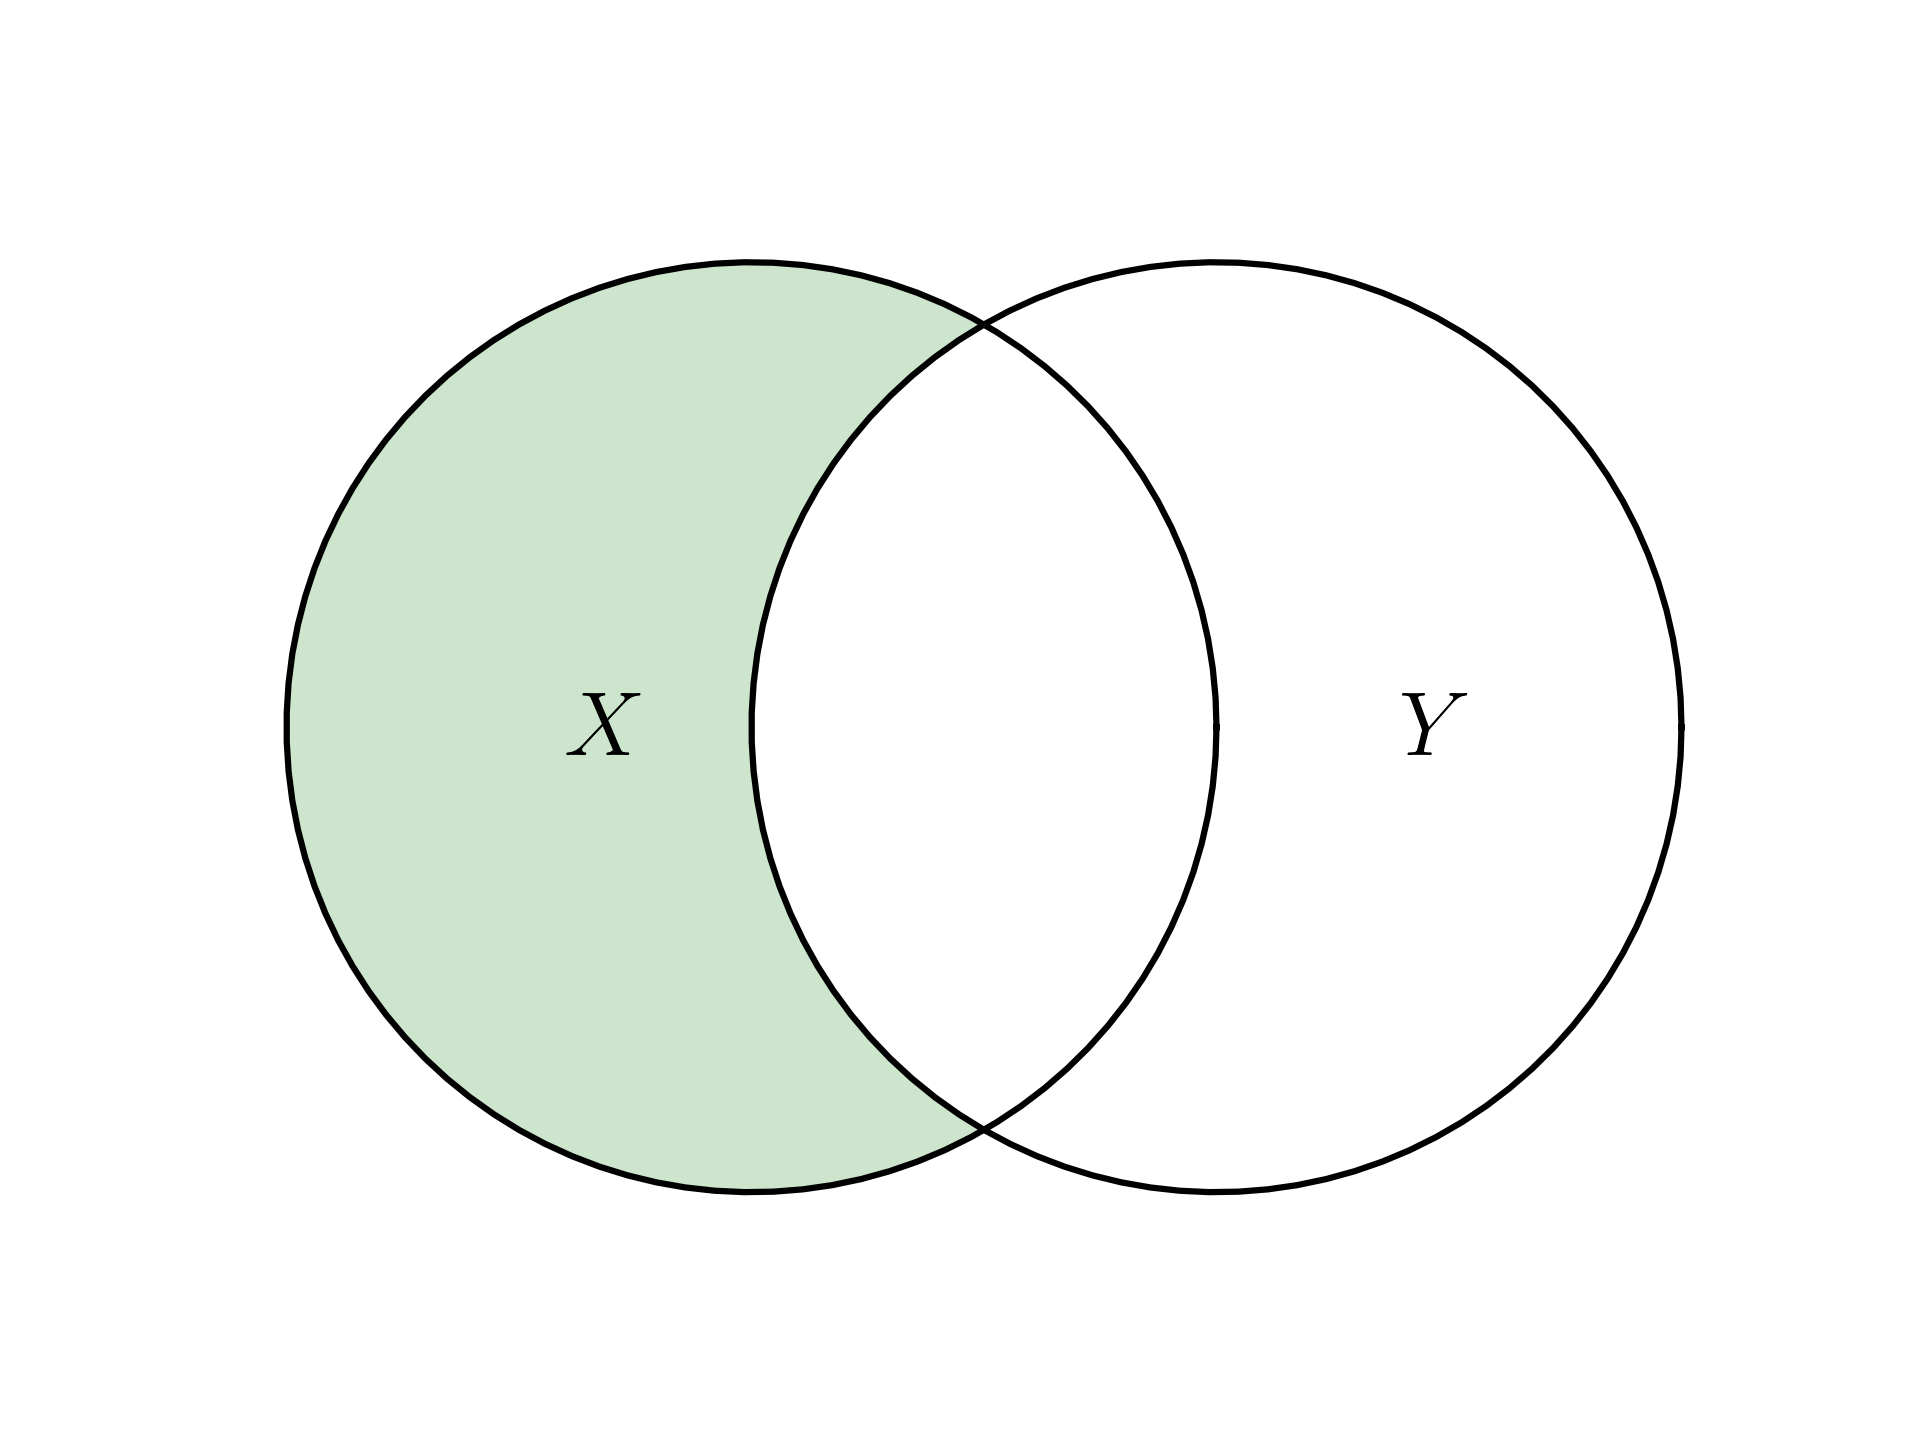
\includegraphics[scale = 0.3]{Figures/graph_difference.png}
\end{center}

\subsubsection{Cartesian product}

If we are given two sets $X$ and $Y$, then their Cartesian product is defined as follows
\[
X \times Y = \{(x, y)\mid x\in X,\;y\in Y\}
\]
The Cartesian product is simply the set of all possible pairs $(x, y)$ where the first element is taken from $X$ and the second from $Y$.
We will use it every time when we need pairs of elements and not just elements.
% TO DO
% Picture

\subsection{Maps}

\begin{definition}
Suppose we are given two sets $X$ and $Y$, a map $f\colon X\to Y$ is a rule that takes elements of $X$ to elements of $Y$.
If $x\in X$, then its image in $Y$ is denoted by $f(x)$.
In this case, we will write $x\mapsto f(x)$.
\end{definition}

The set $X$ is called the source of $f$ and the set $Y$ is called the target of $f$.

Here is a way to think about maps.
Suppose we are given a map $f\colon X\to Y$.
Then $f$ is a callable object with an operator $({-})$.
You give it any element $x$ of $X$, then it returns you some specific element $f(x)$ of $Y$.
For each input $x\in X$, the result $f(x)\in Y$ will be the same every time you call it.
So, a map is the same thing as a function.

\begin{examples}
Here are some examples of maps and non maps.
\begin{enumerate}
\item The rule $f\colon \mathbb R\to \mathbb R$ by $x\mapsto 2 x + 3$ is a map.

\item The rule $f\colon \mathbb R\to \mathbb R$ by $x\mapsto \sin(x)$ is a map.

\item The rule $f\colon \mathbb R\to \mathbb R$ by $x\mapsto \frac{1}{x}$ is not a map because it is not defined at $x = 0$.
It becomes a map if we change the source for $f$.
If $\mathbb R^* = \{x\in \mathbb R\mid x \neq 0\}$, then $f\colon \mathbb R^* \to \mathbb R$ by $x\mapsto \frac{1}{x}$ is a map.

\item The rule $f\colon \mathbb R\to \mathbb R$ by $x\mapsto \ln x$ is not a map because it is only defined for positive $x$.
It becomes a map if we change the source for $f$.
If $\mathbb R_+ = \{x\in \mathbb R\mid x > 0\}$, then $f\colon \mathbb R_+ \to \mathbb R$ by $x\mapsto \ln x$ is a map.
\end{enumerate}
\end{examples}

\section{Binary operations}

The simplest object in Algebra is a set with a good binary operation.
I am going to explain what a binary operation is and the meaning of the word good.
Our goal is to define an object called a Group.

\subsection{Definition}

\begin{definition}
Suppose $X$ is a set.
A binary operation is a map $\circ\colon X\times X\to X$ by the rule $(x, y)\mapsto x\circ y$ for $x, y\in X$.
\end{definition}

In this case the notation $\circ$ is the name of the operation.
Simply speaking, the operation is a rule that takes two elements of the set $X$ and produce a new element called $x\circ y$ of the same set $X$.
This element $x\circ y$ is usually called the product of $x$ and $y$.%
\footnote{The operation could be usual addition of integer numbers or taking maximum between two numbers, but from the general point of view the name of the result is product.
So, mathematics is the art to call different things in a similar way and similar things in a different way.
I will clarify the situation every time when it may lead to confusion.}

You should have noticed that we use the name of the operation in a quite unusual way.
We write the name between the arguments and not before.
This is just for convenience.
However, there is a function-like notation (or map-like notation) for binary operations.
Let me show you

\begin{definition}
Suppose $X$ is a set.
A binary operation is a map $\mu\colon X\times X\to X$ by the rule $(x, y)\mapsto \mu(x, y)$ for $x, y\in X$.
\end{definition}

This is just a different notation for the same mathematical notion.
You may denote an operation in operator-like stile (the first definition) or in a function-like style (the second definition).
To clarify the situation, let me proceed to a series of examples.

\begin{examples}
Binary operations:
\begin{enumerate}
\item Addition of integral numbers.
In an operator-like form
\[
+\colon \mathbb Z\times \mathbb Z\to \mathbb Z,\quad (m,n) \mapsto m + n
\]
In a function-like notation
\[
\operatorname{add}\colon \mathbb Z\times \mathbb Z\to \mathbb Z,\quad (m,n) \mapsto \operatorname{add}(m,n) = m+n
\]
Since we got used to addition of numbers in a form $m + n$, we want a general definition to be in a similar form.
From the other hand, many programming languages allow us using operator-like and function-like notations for addition.
Here I want to emphasize that $\operatorname{add}(m,n)$ and $m+n$ are the same things.
These are just different notations of the same addition that we use with integers.

\item Integer multiplication.
In an operator-like form
\[
\cdot\colon \mathbb Z\times \mathbb Z\to \mathbb Z,\quad (m,n) \mapsto m \cdot n
\]
In a function-like notation
\[
\operatorname{mult}\colon \mathbb Z\times \mathbb Z\to \mathbb Z,\quad (m,n) \mapsto \operatorname{mult}(m,n) = m\cdot n
\]
Again, these are just two different notations for exactly the same operation, that is, multiplication of integer numbers.

\item Integer maximum.
In an operator-like form
\[
\vee\colon \mathbb Z\times \mathbb Z\to \mathbb Z,\quad (m,n) \mapsto m \vee n
\]
In a function-like notation
\[
\operatorname{max}\colon \mathbb Z\times \mathbb Z\to \mathbb Z,\quad (m,n) \mapsto \operatorname{max}(m,n) = m\vee n
\]
Just to clarify $\max(m,n) =m \vee n$ and this is the maximum between $m$ and $n$.

\item Integer minimum.
In an operator-like form
\[
\wedge\colon \mathbb Z\times \mathbb Z\to \mathbb Z,\quad (m,n) \mapsto m \wedge n
\]
In a function-like notation
\[
\operatorname{min}\colon \mathbb Z\times \mathbb Z\to \mathbb Z,\quad (m,n) \mapsto \operatorname{min}(m,n) = m\wedge n
\]
Just to clarify $\min(m,n) =m \wedge n$ and this is the minimum between $m$ and $n$.

\item Some random binary operation on integers
\[
\phi\colon \mathbb Z\times \mathbb Z\to \mathbb Z,\quad (m,n)\mapsto m^2 - n^2
\]
\end{enumerate}
\end{examples}

So, in general a binary operation on $X$ is any map $f\colon X\times X\to X$.
You are free to define it in a way you wish.
But different operations have different properties.
Some of the operations are better than the others in a certain way.
Since we want to deal with good operations only, I am starting a discussion of operation properties.

\subsection{Properties}

There are several properties important for our goal.
I am going to deal with them one-by-one explaining everything on examples.

\subsubsection{Associativity}

\begin{definition}
An operation $\circ \colon X\times X\to X$ is called associative if for every elements $x, y, z\in X$ we have $(x\circ y)\circ z = x\circ (y\circ z)$.
\end{definition}

If you have a binary operation $\circ$ on a set $X$, you can compute the product of three elements $x$, $y$, and $z$ in two different ways:
\begin{itemize}
\item first compute $w = x\circ y$ and then compute $w \circ z = (x\circ y) \circ z$.

\item first compute $u = y \circ z$ and then compute $x \circ u = x \circ (y\circ z)$.
\end{itemize}
If an operation is arbitrary it may happen that these two products are different for some specific elements $x$, $y$, and $z$.
Associativity means that the order of the operations does not matter.
Moreover, if $(x\circ y) \circ z = x \circ (y \circ z)$ for any $x,y,z\in X$, then it does not matter how to place parentheses in any product of elements.
In particular, we may not use parentheses to specify the order, because in general there is no difference between $(x\circ y)\circ (z\circ w)$, $x\circ (y\circ (z\circ  w))$ and $((x\circ  y)\circ z)\circ w$, we may call it simply $x\circ  y \circ z \circ w$.

\begin{examples}
Here are examples of associative and non-associative operations.
\begin{enumerate}
\item Integer addition is associative.
Our operation is
\[
+\colon \mathbb Z\times \mathbb Z\to \mathbb Z,\quad (m,n)\mapsto m+n
\]
Let $m,n,k\in \mathbb Z$ be arbitrary.
Then we know that $(m + n) + k = m + (n + k)$.

\item Integer subtraction is not associative.
Our operation is
\[
-\colon \mathbb Z\times \mathbb Z\to \mathbb Z,\quad (m,n)\mapsto m-n
\]
Then the equality $(m - n) - k = m - (n - k)$ does not hold for any integer numbers.
Indeed, let us take $m = n = 0$ and $k = 1$.
Then the left-hand side is equal to $-1$ and the right-hand side is equal to $1$.
So, $(0 - 0) - 1 \neq 0 - (0 - 1)$.
\end{enumerate}
\end{examples}

\subsubsection{Neutral element}

\begin{definition}
Let $\circ \colon X\times X\to X$ be an operation on $X$.
An element $e\in X$ is called neutral (or identity element) if for every element $x\in X$ we have $x\circ e = x$ and $e \circ x = x$.
\end{definition}

So, a neutral element $e\in X$ is such an element that does not change anything when we multiply by it.

\begin{examples}
A neutral element may exist or may not.
\begin{enumerate}
\item Integral addition has a neutral element.
Our operation is
\[
+\colon \mathbb Z\times \mathbb Z\to \mathbb Z,\quad (m,n)\mapsto m+n
\]
Then it is clear that element $e = 0$ satisfies the required properties.
Indeed, for every natural $m\in \mathbb Z$ we have $m + 0 = m$ and $0 + m = m$.

\item Integer subtraction has no neutral element.
Our operation is
\[
-\colon \mathbb Z\times \mathbb Z\to \mathbb Z,\quad (m,n)\mapsto m-n
\]
Let us show that there is no element $e\in \mathbb Z$ such that $e - m = m$ for every $m\in \mathbb Z$.
Indeed, if such $e$ exists, then $e = 2m$ for any $m\in \mathbb Z$.
But this is impossible because for $m = 0$, $e = 0$ and for $m = 1$, $e = 2$, a contradiction $e$ must be a specific fixed element not depending on $m$.
From the other hand, it is clear that $m - 0 = m$ for any $m\in \mathbb Z$.
\end{enumerate}
\end{examples}

The second example shows that it is not enough to check only one condition $x \circ e = x$ or $e \circ x = x$.
This is a very common mistake to forget one of these conditions.
You are warned!

A reasonable question is: ``How many neutral elements may exist?'' The answer is: ``Not more than one.'' So, there may be no neutral element at all or just one.

\begin{claim}
Let $X$ be a set and $\circ \colon X\times X\to X$ be a binary operation.
Then there exists at most one neutral element.
\end{claim}
\begin{proof}
If there is no neutral elements, we are done.
Suppose that $e$ and $e'$ are neutral elements.
We should show that they are the same.
Consider the product $e \circ e'$.
Since $e$ is a neutral element $e \circ x = x$ for any $x\in X$.
In particular, this holds for $x = e'$, that is, $ e \circ e' = e'$.
From the other hand, since $e'$ is a neutral element $x \circ e' = x$ for any $x\in X$.
In particular, this holds for $x = e$, that is, $e \circ e' = e$.
Thus $e = e\circ e' = e'$.
\end{proof}

\subsubsection{Inverse element}

I want to start with a warning.
This property depends on the previous one, that is, if an operation does not have a neutral element it is impossible to define inverse elements.
This property does not make any sense in case the operation has no neutral element.

\begin{definition}
Let $\circ \colon X\times X\to X$ be an operation such that there is a neutral element $e\in X$.
An element $y\in X$ is called inverse to an element $x\in X$ if $x \circ y = e$ and $y \circ x = e$.
\end{definition}

I want to recall that a neutral element is unique if it exists.
So, element $e$ is well-defined and there is no confusion.

An excellent question is: ``How many inverse elements are there for a particular element $x\in X$?'' The answer is: ``Not more than one if the operation is associative''.
\begin{claim}
Let $\circ \colon X\times X \to X$ be an associative binary operation and $e\in X$ is a neutral element.
Then, every element $x\in X$ has at most one inverse element.
\end{claim}
\begin{proof}
Let us fix an element $x\in X$.
If there is no inverse element for $x$, we are done.
Now, suppose that $y_1$ and $y_2$ are inverse elements for $x$.
The latter means that
\[
\left\{
\begin{aligned}
&x \circ y_1 = e\\
&y_1 \circ x = e
\end{aligned}
\right.
\quad\text{and}\quad
\left\{
\begin{aligned}
&x \circ y_2 = e\\
&y_2 \circ x = e
\end{aligned}
\right.
\]
Now consider the product $y_1 \circ x \circ y_2$.
Since, $\circ$ is associative, it does not matter how to put parentheses, that is $(y_1 \circ x) \circ y_2 = y_1 \circ (x \circ y_2)$.
Let us compute the left-hand side:
\[
(y_1 \circ x) \circ y_2 = e \circ y_2 = y_2
\]
And for the right-hand side, we get
\[
y_1 \circ (x \circ y_2) = y_1 \circ e = y_1
\]
So, $y_2 = (y_1 \circ x) \circ y_2 = y_1 \circ (x \circ y_2) = y_1$ and we are done.
\end{proof}

Hence in general, for every element $x$ if an inverse $y$ exists, then its the only inverse of $x$.
In this case, we denote $y$ as $x^{-1}$.

\begin{examples}
\begin{enumerate}
\item Suppose our operation is an integer addition
\[
+\colon \mathbb Z\times \mathbb Z\to \mathbb Z,\quad (m,n)\mapsto m+n
\]
Then the only neutral element is $0$.
If $n\in \mathbb Z$, then its inverse is $-n$.
Indeed, $n + (-n) = 0$ and $(-n) + n = 0$.
Hence, every element has inverse.

\item Suppose our operation is an integer multiplication
\[
\cdot\colon \mathbb Z\times \mathbb Z\to \mathbb Z,\quad (m,n)\mapsto m\cdot n
\]
The only neutral element is $	1$.
If $n = 1$, then its inverse is $1$.
If $n = -1$, then its inverse is $-1$.
If $n\neq \pm1$, then there is no inverse in $\mathbb Z$.
Indeed, if $n = 2$, then there is no integer $m$ such that $nm = 2m = 1$.
Hence, only two elements have inverse.
\end{enumerate}
\end{examples}

\subsubsection{Commutativity}

\begin{definition}
A binary operation $\circ \colon X\times X\to X$ is called commutative if, for every $x,y\in X$, we have $x \circ y = y\circ x$.
\end{definition}

So, commutativity means that the order of operands does not matter.

\begin{examples}
\begin{enumerate}
\item Integral addition is commutative.
Our operation is
\[
+\colon \mathbb Z\times \mathbb Z\to \mathbb Z,\quad (m,n)\mapsto m+n
\]
Let $m,n\in \mathbb Z$ be arbitrary.
Then we know that $m + n = n + m$.

\item Integer subtraction is not commutative.
Our operation is
\[
-\colon \mathbb Z\times \mathbb Z\to \mathbb Z,\quad (m,n)\mapsto m-n
\]
Then the equality $m - n = n - m$ does not hold for any integer $m,n$.
Indeed, if $m = 0$ and $n = 1$, then the left-hand side is $-1$ and the right-hand side is $1$.
\end{enumerate}
\end{examples}

\section{Groups}

\subsection{Definition}

Now we are ready to give the most important definition in Algebra, that is the definition of a Group.
Before we proceed, I want to clarify the general structure of definitions in Algebra.
Every definition of an abstract object consists of two parts: 1) in the first part we list all the data required for the definition, 2) in the second part we list all the axioms the data must satisfy.

\begin{definition}
Definition of a group.
\begin{itemize}
\item\textbf{Data:} 
\begin{enumerate}
\item A set $G$.

\item An operation $\circ \colon G\times G\to G$.
\end{enumerate}
\item\textbf{Axioms:}
\begin{enumerate}
\item The operation $\circ$ is associative.

\item The operation $\circ$ has a neutral element.

\item Every element $x\in G$ has an inverse.
\end{enumerate}
\end{itemize}
In this case, we say that the pair $(G, \circ)$ is a group.
In order to simplify the notation, we usually say simply that $G$ is a group assuming that the operation in use is clear.
If in addition we have
\begin{itemize}
\item[]
\begin{enumerate}
\setcounter{enumi}{3}
\item The operation $\circ$ is commutative.
\end{enumerate}
\end{itemize}
Then the group $G$ is called abelian or simply commutative.
\end{definition}


In short, a group is a set with a good operation.
Here, good means that we do not care about parentheses, we have neutral element and every element is invertible but the order of the elements still matters.
Abelian group means that additionally the order of the elements does not matter.

\begin{examples}
\begin{enumerate}
\item Integers with addition $(\mathbb Z, +)$ is an abelian group.
Indeed, the operation $+$ is associative, has an identity element $0$, every element $n$ has inverse $-n$ and the order in addition does not matter, that is $n + m = m + n$.
We usually call this group simply $\mathbb Z$ assuming the addition as our operation by default.

\item Integers with multiplication $(\mathbb Z, \cdot)$ is not a group.
Indeed, the operation $\cdot$ is associative, has an identity element $1$, but there are a lot of non-invertible elements (the only invertible elements are $\pm1$).

\item Non-zero real numbers with multiplication $(\mathbb  R^*, \cdot)$ is an abelian group.
Indeed, the operation $\cdot$ is associative, has an identity element $1$, every element $x$ as inverse $1/x$, and the order in multiplication does not matter, that is $xy = yx$.

\item Let $n$ be any positive integer, then the set $\mathbb Z_n = \{0,1, \ldots, n-1\}$ with operation $a + b \pmod n$ is an abelian group.
The operation on $\mathbb Z_n$ we will simply be denote by $+$.

\item Let $n$ be any positive integer and $\mathbb Z_n^* = \{m\in \mathbb Z_n \mid (m,n) = 1\}$ (that is the set of all integers in $\mathbb Z_n$ coprime with $n$) with operation $a \cdot b \pmod n$ is an abelian group.
The operation on  $\mathbb Z_n^*$ will simply be denoted by $\cdot$.

\end{enumerate}
\end{examples}

\subsection{Multiplicative and additive notations}

If we are given a group $G$, we usually denote its operation by $\circ$.
However, it is very cumbersome to use this notation.
Instead, people use symbols for usual multiplication or addition and there are two different types of notation: multiplicative and additive.
Let me introduce the notation
\begin{center}
\begin{tabular}{c|c|c|c}
{}&{Multiplicative}&{Additive}\\
\hline
{Operation}&{$\cdot \colon G\times G\to G$}&{$+\colon G\times G\to G$}\\
{On elements}&{$(x, y)\mapsto xy$}&{$(x,y)\mapsto x+y$}\\
{Neutral Element}&{$1$}&{$0$}\\
{Inverse Element}&{$x^{-1}$}&{$-x$}\\
{Power of Element}&{$x^n = \underbrace{x \cdot\ldots \cdot x}_n$}&{$nx = \underbrace{x + \ldots + x}_n$}\\
\end{tabular}
\end{center}
Usually the multiplicative notation is used in case of an arbitrary non-abelian group and the additive notation is used in case of an abelian group.
I will mostly stick to the multiplicative notation and use the additive only in case of abelian groups.

I want to emphasize that these are just two different notations for the operation $\circ$.
That is $xy = x\circ y$ or $x + y = x\circ y$.
You just denote $\circ$ by $\cdot$ or $+$ depending on your preferences.
Do not confuse these notations with the usual multiplication and addition.
In case of an arbitrary group $G$, there is no confusion because there is no addition and multiplication on an arbitrary set $G$.
However, If we deal with integer numbers (real, rational, complex, etc.), the operations $+$ and $\cdot$ denote usual addition and multiplication.

\subsection{Subgroups}

\begin{definition}
Let $G$ be a group.%
\footnote{Strictly speaking $(G,\cdot)$ but I am going to use the short notation all the time.}
We define a subgroup $H$ of $G$.
\begin{itemize}
\item \textbf{Data:} 
\begin{enumerate}
\item A subset $H\subseteq G$.
\end{enumerate}
\item \textbf{Axioms:}
\begin{enumerate}
\item The neutral element $1$ of $G$ belongs to $H$.

\item $x  y\in H$ whenever $x,y\in H$.

\item $x^{-1}\in H$ whenever $x\in H$.
\end{enumerate}
\end{itemize}
In this case, we say that $H$ is a subgroup of $G$.
\end{definition}

It should be noted that if $H$ is a subgroup of $G$, then $\cdot$ is a well-defined operation on $H$ and $(H,\cdot)$ becomes a group.

\begin{examples}
Let $G =\mathbb Z$ with addition.
\begin{enumerate}
\item If $H\subseteq \mathbb Z$ is the set of even numbers, that is $H = 2\mathbb Z$, then $H$ is a subgroup.

\item If $H\subseteq \mathbb Z$ is the set of odd numbers, that is $H = 1 + 2 \mathbb Z$, then $H$ is not a subgroup.
For example, the neutral element $0$ is not in $H$.
Also, $H$ is not closed under addition.
\end{enumerate}
\end{examples}

\subsection{Cyclic subgroups}

Let $G$ be a group and $g\in G$ be an arbitrary element.
Then we may take any integer power of $g$ as follows
\begin{center}
\begin{tabular}{c | c}
{Multiplicative notation}&{Additive notation}\\
\hline
{
$
g^n =
\left\{
\begin{aligned}
&\underbrace{g\cdot \ldots \cdot g}_n,&&n>0\\
&1,&&n=0\\
&\underbrace{g^{-1}\cdot \ldots \cdot g^{-1}}_{-n},&&n<0\\
\end{aligned}
\right.
$
}&{
$
n g =
\left\{
\begin{aligned}
&\underbrace{g+ \ldots + g}_n,&&n>0\\
&0,&&n=0\\
&\underbrace{(-g) + \ldots +(- g)}_{-n},&&n<0\\
\end{aligned}
\right.
$
}\\
\end{tabular}
\end{center}

\begin{claim}
Let $G$ be a group.
Then
\begin{enumerate}
\item For any $x,y\in G$, $(xy)^{-1} = y^{-1}x^{-1}$.

\item For any $g\in G$, $(g^{-1})^n = (g^n)^{-1}$.

\item For any $g\in G$, $g^n g^m = g^{n+m}$ whenever $n,m\in \mathbb Z$.
\end{enumerate}
\end{claim}
\begin{proof}
1) We need to show that $(xy)^{-1} = y^{-1}x^{-1}$.
Let us denote $ y^{-1}x^{-1}$ by $z$.
If we show that $(xy)z = z(xy) = 1$, this will mean that $z = (xy)^{-1}$ by definition.
Now, we compute
\[
(xy) z = xy z = xy y^{-1}x^{-1} = x x^{-1} = 1
\]
In a similar way, we show the other equality.

2) We apply the previous property several times, that is
\[
(g_1\cdot \ldots \cdot g_n)^{-1} = g_n^{-1}\cdot\ldots\cdot g_1^{-1},\;\text{ whenever }g_1,\ldots,g_n\in G
\]
If we substitute $g_1 =\ldots = g_n = g$, this proves the required for $n > 0$.

If $n = 0$, then by definition $(g^{-1})^0 = 1$.
From the other hand, $(g^0)^{-1} = 1^{-1} = 1$ because the inverse for $1$ is $1$.

If $n < 0$, then by definition
\[
(g^{-1})^n = \underbrace{(g^{-1})^{-1}\cdot\ldots \cdot (g^{-1})^{-1}}_{-n}
\]
On the other hand, 
\[
(g^n)^{-1} = (\underbrace{g^{-1}\cdot \ldots \cdot g^{-1}}_{-n})^{-1} = \underbrace{(g^{-1})^{-1}\cdot\ldots \cdot (g^{-1})^{-1}}_{-n}
\]
The latter equality follows from the previous item.

3) We should consider $4$ cases:
\begin{enumerate}
\item $n\geqslant 0$ and $m\geqslant 0$.

\item $n < 0$ and $m\geqslant 0$.

\item $n\geqslant 0$ and $m < 0$.

\item $n < 0$ and $m < 0$.
\end{enumerate}
In the first case, we have
\[
g^n g^m = \underbrace{g\cdot \ldots \cdot g}_n\cdot\underbrace{g\cdot \ldots \cdot g}_m = \underbrace{g\cdot \ldots \cdot g}_{n+m} = g^{n+m}
\]
For convenience, we consider $g^{-n} g^{m}$ for $n>0$ and $m\geqslant 0$ in the second case.
\[
g^{-n}g^{m} = \underbrace{g^{-1}\cdot \ldots \cdot g^{-1}}_{n}\cdot\underbrace{g\cdot \ldots \cdot g}_m
\]
We cancel the factors at the middle of the expression.
If $n >m$, we get
\[
\underbrace{g^{-1}\cdot \ldots \cdot g^{-1}}_{n - m} = g^{-n + m}
\]
If $n < m$, we get
\[
\underbrace{g\cdot \ldots \cdot g}_{m - n} = g^{m - n}
\]
if $n = m$ we get $1 = g^{m - n}$.
Other cases I leave as an exercise.
\end{proof}


\begin{definition}
Let $G$ be a group and $g\in G$ be an arbitrary element.
Then the set of all integer powers of $g$, that is,
\[
\langle g \rangle = \{ \ldots, g^{-2},g^{-1},1, g, g^2, \ldots\}
\]
is a subgroup of $G$.
This group is called the cyclic subgroup generated by $g$.
The element $g$ is called a generator of $\langle g\rangle$.
\end{definition}

The cyclic subgroup $\langle g\rangle$ is the smallest possible subgroup containing the element $g$.

\begin{examples}
\begin{enumerate}
\item The group $(\mathbb Z, +)$ is cyclic.
There are two different generators $1$ and $-1$.

\item The group $(\mathbb Z_n, +)$ is cyclic.

\item The group of permutations on $n$ elements $S_n$ is not cyclic if $n >2$.

\item The group $(\mathbb R, +)$ is not cyclic.
\end{enumerate}
\end{examples}

\begin{claim}
\label{claim::CyclicClass}
Let $G$ be a group and $g\in G$ be an arbitrary element.
Then there are two options:
\begin{itemize}
\item If $\ord g = \infty$, then the elements $g^n$ and $g^m$ are different whenever $n,m\in\mathbb Z$ are different.

\item If $\ord g = n < \infty$, then elements $1, g, g^2, \ldots, g^{n-1}$ are different.
In this case, the powers are repeated in cycles, that is in the series 
\[
\underbrace{\ldots, g^{-2},g^{-1}},\underbrace{1, g, g^2, \ldots, g^{n-1}}, \underbrace{g^n, g^{n+1},\ldots,g^{2n - 1}}, \underbrace{g^{2n},\ldots}\\
\]
$g^{kn}, g^{1 + kn}, \ldots, g^{n-1 + nk}$ are the same elements as $1, g, \ldots, g^{n-1}$ for any $k\in \mathbb Z$.
In particular, 
\[
\langle g\rangle =\{1,g,\ldots g^{n-1}\}
\]
\end{itemize}
\end{claim}
\begin{proof}
If $g^n\neq g^m$ for all different $m,n\in \mathbb Z$, we are in the first case.

Now suppose that $g^n = g^m$ for some integer $m\neq n$.
Then we may multiply this equality by $g^{-m}$ and get $g^{n-m} = 1$.
Hence, we may assume that for some $n \neq 0$, we have $g^n = 1$.
If $n < 0$, multiply by $g^{-n}$.
Thus, we may assume that for some positive integer $n$, we have $g^n = 1$.

Consider the minimal positive integer $n$ such that $g^n = 1$.
I claim that the elements $1, g, \ldots, g^{n-1}$ are different.
Indeed, if $g^k = g^s$ for some $k,s \in [0, n-1]$ and $k \geqslant s$, then $g^{k-s} = 1$ and $k - s$ is not zero and is strictly less than $n$.
The latter contradicts to the choice of $n$.
\end{proof}

It should be noted that $n$ may equal $1$ in case $g$ is the neutral element $1$.

\begin{definition}
Let $G$ be a group and $g\in G$ be an arbitrary element.
The order of $g$ is the minimal positive natural number such that $g^n = 1$ and $\infty$ if there is no such a number.
The order of $g$ is denoted by $\ord g$.
\end{definition}

From the previous Claim it follows that $\ord g$ equals the number of elements in $\langle g\rangle$.
Note that $g  = 1$ if and only if $\ord g = 1$.

If we use additive notation, that is the operation on the group $G$ is denoted by $+$, then, the order of $g\in G$ is the small positive integer $n$ such that $ng = 0$.
The cyclic subgroup generated by $g$ is
\[
\langle g\rangle = \{\ldots, -2 g, - g , 0, g, 2g, \ldots\}
\]

\begin{definition}
Let $G$ be a group.
If there is an element $g\in G$ such that $\langle g\rangle = G$, then the group $G$ is called cyclic.
\end{definition}

\ProvidesFile{lecture02.tex}[Lecture 2]


Now, I want to describe all subgroups of the integers with addition.

\begin{claim}
\label{claim::Zsubgroups}
Every subgroup $H$ of $\mathbb Z$, that is $(\mathbb Z, +)$, is of the form $k\mathbb Z$ for some natural $k$.
\end{claim}
\begin{proof}
Let us check that $k \mathbb Z$ is indeed a subgroup for any $k$.
We need to check three properties of the subgroup.
First, $k\mathbb Z$ is closed under addition.
But this is clear by definition.
Second, the neutral element, which is zero, belongs to $k\mathbb Z$.
This is also clear since $0 = k \cdot 0$.
Third, for each $m = kh \in k\mathbb Z$, its inverse $-m= k(-h)$ is also in $\mathbb Z$, and we are done with this part.

Now, let us check that every subgroup $H$ is of the form $k \mathbb Z$.
If $H$ contains only the neutral element $0$, then $H = 0\mathbb Z$ and we are done.
Suppose $H$ contains non-zero elements.
Take an arbitrary non-zero $n \in H$.
If $n < 0$, then $-n$ must belong to $H$ by definition of a subgroup.
And hence, we may assume that $H$ contains some positive numbers.
Let $k$ be the smallest positive number in $H$.
Let us show that $H = k \mathbb Z$.

First, $H \supseteq k \mathbb Z$.
Indeed, if $k\in H$, then by definition of a subgroup every ``power'' of $k$ is in $H$.
For additive notation this means 
\[
mk  = \underbrace{k + \ldots + k}_m \in H\;\text{ and }\;(-n)k=\underbrace{(-k) + \ldots + (-k)}_n\in H\; \text{ for any }\;m, n\in \mathbb N
\]
Hence, $k\mathbb Z\subseteq H$.

Now, let us show that $H\subseteq k\mathbb Z$.
If $n\in H$ is an arbitrary element, let us divide $n$ by $k$: $n = q k + r$, where $q\in \mathbb Z$ and $0 \leqslant r < k$.
We already know that $qk \in k\mathbb Z\subseteq H$, that is $qk \in H$.
Hence, $r = n - qk \in H$.
But $r$ is a natural number in $H$ smaller than $k$.
Since $k$ is the smallest positive in $H$, the only option is $r = 0$.
Thus, $n = qk\in k\mathbb Z$ and we are done.
\end{proof}

\begin{claim}
\label{claim::Znsubgroups}
Every subgroup $H$ of $\mathbb Z_n$, that is $(\mathbb Z_n, +)$, is of the form $k\mathbb Z_n =\{kh\in \mathbb Z_n \mid h\in \mathbb Z_n\}$ for some positive $k \mid n$.
\end{claim}
\begin{proof}
First, let us check that all numbers divisible by $k$ such that $k\mid n$ form a subgroup in $\mathbb Z_n$.
First, we need to check that $k\mathbb Z_n$ is closed under addition modulo $n$.
Suppose $m_1 = k h_1$ and $m_2 = k h_2$ are elements of $k \mathbb Z_n$.
Then their sum modulo $n$ is a remainder $r$ such that $ m_1+ m_2 = r \pmod{n}$.
In this case,
\[
r = m_1 + m_2 + q n = k h_1 + kh_2 + qn
\]
Since $k$ divides $n$ the whole expression above is divisible by $k$.
Hence $r$ is divisible by $k$.
The latter means that $k \mathbb Z_n$ is closed under addition modulo $n$.
Second, we need to check that $k\mathbb Z_n$ contains the neutral element.
This is clear, since $0 = k \cdot 0\in k\mathbb Z_n$.
Third, if $m\in k\mathbb Z_n$ is a nonzero element, then its inverse is $n - m$.
Since $n$ is divisible by $k$, $n-m$ is divisible by $k$.
Hence, it belongs to $k\mathbb Z_n$.
In case $m = 0$ its inverse is $0$ and is already in $k \mathbb Z_n$.
Hence, for each $k\mod n$, $k\mathbb Z_n$ is a subgroup of $\mathbb Z_n$.

Now, let us show, that every subgroup $H$ in $\mathbb Z_n$ coincides with a subgroup of the form $k\mathbb Z_n$ for $k\mid n$.
The subgroup $H$ must contain the neutral element $0$.
If this is the only element of $H$, then $H = \{0\} = n \mathbb Z_n$ and we are done.
So, we may suppose there is a non-zero, and hence positive, element in $H$.
Let $k$ be the smallest positive element of $H$.
By definition the cyclic subgroup of $k$, that is $k\mathbb Z_n$, belongs to $H$.
Thus, we need to show, that $H\subseteq k \mathbb Z_n$ and $k$ divides $n$.

First, let me show that $k$ divides $n$.
Let us divide $n$ with remainder by $k$, we will get $n = qk + r$, where $0\leqslant r < k$.
Now, $r = n - q k$, hence $r = -q k \pmod{n}$.
Since $k\in H$, the latter means that $r$ is also in $H$.
But this contradicts the choice of $k$ (it was the smallest nonzero integer in $H$).
Hence, $r$ must be zero, thus $k$ divides $n$.
Second, let me show that every element of $H$ is in $k\mathbb Z_n$.
Suppose $h\in H$ is an arbitrary element.
Let us divide $h$ with remainder by $k$, we will get $h = q k + r$.
Hence, $r = h - q k$.
Since $h\in H$ and $k\in H$, the whole expression $h - qk$ is in $H$.
Hence, $r\in H$.
Since $k$ was the smallest positive integer of $H$, we must have $r = 0$.
The latter means that $h$ is divisible by $k$, that is, $h$ belongs to $k\mathbb Z_n$, and we are done.
\end{proof}

\subsection{Cosets}

Algebra usually tends to study groups using subgroups rather than elements.
The main tool here is cosets.

\begin{definition}
Let $G$ be a group, $H\subseteq G$ a subgroup and $g\in G$ an arbitrary element.
Then the set
\[
gH = \{gh\mid h\in H\}
\]
is called the left coset of $H$ with respect to $g$.
In a similar way, we define right cosets.
The set
\[
Hg = \{hg\mid h\in H\}
\]
is called the right coset of $H$ with respect to $g$.
\end{definition}

\begin{remarks}
\begin{enumerate}
\item It should be noted that if $G$ is commutative, then there is no difference between left and right cosets for any subgroup $H\subseteq G$.

\item The group $H$ itself is a left coset as well as a right coset.
Indeed, $H = 1 \cdot H = H \cdot 1$.

\item In general, the left cost $gH$ need not be the same as the right coset $Hg$ as an example below shows.
\end{enumerate}
\end{remarks}


\begin{examples}
Here are some examples of cosets.
\begin{enumerate}
\item Let $G = (\mathbb Z, +)$ and $H = 2\mathbb Z$ the subgroup of even numbers.
Then $2\mathbb Z$ and $1 + 2\mathbb Z$ are the only cosets of $H$.

\item Let $G = S_3$ and $H = \langle (1, 2)\rangle$ the cyclic subgroup generated by the cycle $(1,2)$.
We may list all the elements of $G$ and $H$
\[
G = \{1, (1,2), (1, 3), (2, 3), (1, 2, 3), (3, 2, 1)\},\; H = \{1, (1, 2)\}
\]
Then there are three different left cosets of $H$
\[
H = \{1, (1, 2)\}, \;(1,3)H = \{(1, 3), (1, 2, 3)\},\;(2, 3)H = \{(2, 3), (3,2,1)\}
\]
And there are three different right cosets of $H$
\[
H =  \{1, (1, 2)\}, \; H(1, 3) = \{(1, 3), (3, 2, 1)\},\; H (2, 3) = \{(2, 3), (1, 2, 3)\}
\]
This example shows that $(1, 3) H \neq H (1, 3)$.
Also, it should be noted that
\[
(1, 2)H = H,\; (1, 3)H = (1, 2, 3)H,\; (2, 3)H = (3, 2, 1)H
\]
So, cosets with respect to different elements may be the same.

\item Let $G = S_n$ be the group of permutations on $n$ elements and $H = A_n$ be the subgroup of even permutations.
Then, for any even permutation $\sigma\in A_n$, the set $\sigma A_n$ consists of all even permutations.
Similarly, for any odd permutation $\sigma\in S_n\subseteq A_n$, the set $\sigma A_n$ consists of all odd permutations.
Hence, there are only two left cosets of $A_n$
\[
A_n\;\text{and}\;(1, 2) A_n
\]
In a similar way, we can show that there are only two right cosets of $A_n$
\[
A_n\;\text{and}\; A_n(1, 2)
\]
Moreover, we have shown that $\sigma A_n = A_n \sigma$ for any $\sigma \in S_n$.
\end{enumerate}
\end{examples}

\begin{definition}
Let $G$ be a group and $H$ its subgroup.
The subgroup $H$ is normal if its left and right cosets are the same, that is, $gH = Hg$ whenever $g\in G$.
\end{definition}

\begin{claim}
\label{claim::normal_crit}
Let $G$ be a group and $H$ its subgroup.
Then, the following are equivalent
\begin{enumerate}
\item $gH = Hg$ for each $g\in G$.

\item $gHg^{-1} = H$ for each $g\in G$.

\item $gHg^{-1}\subseteq H$ for each $g\in G$.
\end{enumerate}
\end{claim}
\begin{proof}
(1)$\Leftrightarrow$(2).
Suppose $gH = Hg$.
Multiply this on the right by $g^{-1}$ and get $gH g^{-1} = H$.
And if we are given $g H g^{-1} = H$, multiply this on the right by $g$ and get $gH = Hg$.

(2)$\Leftrightarrow$(3).
We should show that $gHg^{-1}\subseteq H$ for each $g\in G$ implies  $gHg^{-1} = H$ for each $g\in G$.
The other implication is clear.
If  $gHg^{-1}\subseteq H$ for each $g\in G$, then it holds for $g^{-1}$ instead of $g$.
Thus, $g^{-1}Hg \subseteq H$ for each $g\in G$.
Multiply this on the left by $g$ and get $Hg \subseteq gH$.
Then, multiply the latter on the right by $g^{-1}$ and get $H \subseteq gH g^{-1}$.
Since $g\in G$ was arbitrary we are done.

\end{proof}

\subsection{The Lagrange Theorem}

\paragraph{Properties of cosets}

Now, I want to prove several properties of the cosets.
The important observation here is that all left cosets form a partition of the group $G$ into non-overlapping subsets.
The same is true for the right cosets.
This observation provides us with some combinatorial tools.


\begin{claim}
\label{claim::cosets_disj}
Let $G$ be a group, $H\subseteq G$ a subgroup and $g_1, g_2\in G$ be arbitrary elements.
Then there are two options:
\begin{enumerate}
\item The cosets do not intersect each other: $g_1 H \cap g_2 H = \varnothing$.

\item The cosets coincide: $g_1 H = g_2 H$.
\end{enumerate}
This means that each element of the group $G$ belongs to exactly one coset.
\end{claim}
\begin{proof}
If $g_1H$ does not intersect $g_2H$ there is nothing to prove.

Now we assume that the intersection $g_1 H\cap g_2 H$ is not empty.
We need to prove that $g_1 H = g_2 H$.
Suppose $g\in g_1 H \cap g_2H$.
Since $g\in g_1H$, $g = g_1 h_1$ for some $h_1\in H$.
Similarly, $g\in g_2H$ implies $g = g_2 h_2$ for some $h_2\in H$.
Hence $g_1 h_1 = g_2 h_2$.
Dividing by $h_1$ on the right, we get $g_1 = g_2 h_2 h_1^{-1}$.
Since $H$ is a subgroup $h = h_2 h_1^{-1}\in H$.
We have got $g_1 = g_2 h$ for some $h\in H$.

Let us show that $g_1 H \subseteq g_2 H$.
Suppose $g\in g_1H$, that is $g = g_1 h'$ for some $h'\in H$.
Then, $g =g_2 h h'\in g_2 H$ because $hh'\in H$.
Now, suppose $g\in g_2H$, that is $g = g_2 h'$ for some $h'\in H$.
Then, $g = g_1 h^{-1}h'\in g_1 H$ because $h^{-1}h'\in H$.
Hence, we have shown $g_2 H \subseteq g_1 H$.
\end{proof}

\begin{remark}
It should be noted that $g_1 H  = g_2H$ if and only if $g_1 H \cap g_2 H \neq \varnothing$.
Moreover, this occurs if and only if there is an element $h\in H$ such that $g_1 = g_2 h$.
The latter is equivalent to the condition $g_2^{-1}g_1 \in H$.
This provides us with a convenient way of checking if two cosets are the same.
\end{remark}

\begin{claim}
\label{claim::cosets_size}
Let $G$ be a group, $H\subseteq G$ be a finite subgroup and $g\in G$ an arbitrary element.
Then $|gH| = |H| = |Hg|$.
\end{claim}
\begin{proof}
I will prove the claim for left cosets.
Let us consider the map
\[
\phi \colon H \to g H\quad x \mapsto gx
\]
It takes elements of $H$ to elements of $gH$.
From the other hand, there is the inverse map
\[
\psi \colon gH \to H\quad x \mapsto g^{-1}x
\]
Thus $\phi$ and $\psi$ are bijections and we are done.
\end{proof}

\begin{claim}
\label{claim::cosets_l_r_same}
Let $G$ be a finite group and $H\subseteq G$ be a subgroup.
Then
\begin{enumerate}
\item The amount of left cosets of $H$ is equal to $|G|/|H|$.

\item The amount of right cosets of $H$ is equal to $|G|/|H|$.
\end{enumerate}
In particular, the number of left and right cosets is the same.
\end{claim}
\begin{proof}
We will prove the first item.
Claim~\ref{claim::cosets_disj} shows that $G$ is a disjoint union of some cosets, that is $G = g_1 H \sqcup \ldots \sqcup g_k H$.
From the other hand, Claim~\ref{claim::cosets_size} shows that all the cosets $g_1H,\ldots, g_kH$ have the same amount of elements being equal to $|H|$.
Hence 
\[
|G| = |g_1H| + \ldots +|g_k H| = |H| + \ldots + |H| = k |H|
\]
Here $k$ is the number of the distinct left cosets and we are done.
\end{proof}

\begin{definition}
Let $G$ be a finite group and $H\subseteq G$ be a subgroup.
Then the number of the left cosets of $H$ is called index of $H$ and is denoted by $(G:H)$.
This number is also coincide with the number of the right cosets of $H$.
\end{definition}

Using this notation, we can rewrite Claim~\ref{claim::cosets_l_r_same} in the following way.

\begin{claim}
[The Lagrange Theorem]
Let $G$ be a finite group and $H\subseteq G$ be a subgroup.
Then, $|G| = (G : H)|H|$
\end{claim}


\paragraph{Corollaries of The Lagrange Theorem}

\begin{enumerate}
\item Let $G$ be a finite group and $H\subseteq G$ be a subgroup.
Then $|H|$ divides $|G|$.

\item Let $G$ be a finite group and $g\in G$ be an arbitrary element.
Then $\ord(g)$ divides $|G|$.
Indeed, $\ord(g) = |\langle g \rangle|$.
But $|\langle g\rangle|$ divides $|G|$ by the previous item.

\item Let $G$ be a finite group and $g\in G$ be an arbitrary element.
Then $g^{|G|} = 1$.
Indeed, we already know that $|G| = \ord(g) k$.
Hence, 
\[
g^{|G|} = g^{\ord(g)k} = \left(g^{\ord(g)}\right)^{k} = 1^k = 1
\]

\item Let $G$ be a group of prime order $p$.
Then, $G$ is cyclic.
Indeed, since the order of $G$ is prime, it is greater than $1$.
Hence, there is an element $g\in G$ such that $g\neq 1$.
Hence $\langle g\rangle$ has order greater than $1$.
But $|\langle g \rangle|$ divides $|G| = p$.
Since $p$ is prime, the only option is $|\langle g \rangle| = p = |G|$.
The latter means that $\langle g \rangle = G$ and we are done.

\item The Fermat Little Theorem.
Let $p\in \mathbb Z$ be a prime number and $a\in \mathbb Z$.
If $p$ does not divide $a$, then $p$ divides $a^{p-1}-1$.
Indeed, let us consider the group $(\mathbb Z_p^*, \cdot)$.
For any element $b\in \mathbb Z_p^*$, we have $b^{|\mathbb Z_p^*|} = 1 \pmod p$ by item~(3).
But $\mathbb Z_p^*$ has $p-1$ elements.
Now, let $a\in \mathbb Z$ be comprime with $p$.
We denote its remainder modulo $p$ by $b$.
Then $a^{p-1} = b^{p-1} = 1\pmod p$ and we are done.
\end{enumerate}

\ProvidesFile{lecture03.tex}[Lecture 3]


\subsection{Homomorphisms and Isomorphisms}

We have a lot of different groups in algebra.
And we will study a couple of ways to produce new groups from given ones.
In this situation, we need a way to compare the groups.
How to recognize that we have constructed the same group that we already know?
In order to answer this question, we need to explain what it means that two groups are the same.
So, we need a way to compare two groups.
This leads us to the notions of homomorphism (a way to compare groups) and isomorphism (a way to say that groups are the same).
Let me proceed with formal definitions.

\begin{definition}
Let $G$ and $H$ be groups.
We define a homomorphism $\varphi\colon G\to H$.
\begin{itemize}
\item \textbf{Data} A map $\varphi\colon G\to H$.

\item \textbf{Axiom} $\varphi(g_1g_2) = \varphi(g_1) \varphi(g_2)$ for any $g_1,g_2\in G$.
\end{itemize}
In this case $\varphi$ is called a homomorphism from $G$ to $H$.
\end{definition}

\begin{remark}
Let me explicitly repeat the definition.
We are given a group $(G, \circ)$ and $(H,\cdot)$.
A homomorphism $\varphi \colon G\to H$ is a map such that $\varphi(g_1 \circ g_2) = \varphi(g_1) \cdot \varphi(g_2)$.
On the left-hand side we take elements $g_1$ and $g_2$ from $G$ and multiply them using the operation on $G$ and then send the resulting element to $H$.
On the right-hand side, we send the elements $g_1$ and $g_2$ to the group $H$ first and then multiply the images using operation on $H$.
\end{remark}

\begin{examples}
\begin{enumerate}
\item Let $G = (\mathbb Z, +)$ and $H = (\mathbb Z_n, +)$, then the map $\pi\colon \mathbb Z\to \mathbb Z_n$ by the rule $k \mapsto k \pmod n$ is a homomorphism.

\item Let $G = S_n$ be the group of permutations and $H = \mu_2 = \{\pm 1\}$ with multiplication.
Then the map $\sgn \colon S_n \to \mu_2$ taking each permutation to its sign (even one goes to $1$ and odd one goes to $-1$) is a homomorphism.

\item Let $G = (\operatorname{GL}_n(\mathbb R),\cdot)$ and $H = (\mathbb R^*, \cdot)$ be the set of non-zero real numbers with multiplication.
Then the map $\det \colon \operatorname{GL}_n(\mathbb R) \to \mathbb R^*$ by the rule $A \mapsto \det(A)$ is a homomorphism.

\item Let $G = (\mathbb R, +)$ and $H = (\mathbb R^*, \cdot)$.
Then the map $\exp\colon \mathbb R\to \mathbb R^*$ by the rule $x \mapsto e^x$ is a homomorphism.

\item Let $G = (\mathbb Z, +)$, $H$ be an arbitrary group and $h\in H$ be an arbitrary element.
Then the map $\phi\colon \mathbb Z \to H$ by the rule $k \mapsto h^k$ is a homomorphism.

\item Let $G = (\mathbb Z_n, +)$, $H$ be an arbitrary group and $h\in H$ be an element such that $h^n = 1$.
Then the map $\phi\colon \mathbb Z_n \to H$ by the rule $k \mapsto h^k$ is a group homomorphism.
\end{enumerate}
\end{examples}

Let us prove several properties of homomorphisms.

\begin{claim}
\label{claim::HomGrProp}
Let $\varphi\colon G\to H$ be a homomorphism of groups.
Then
\begin{enumerate}
\item $\varphi(1) = 1$, that is the neutral element of $G$ goes to the neutral element of $H$.

\item $\varphi(g^{-1}) = \varphi(g)^{-1}$ whenever $g\in G$.
\end{enumerate}
\end{claim}
\begin{proof}
1) We know that $1 = 1 \cdot 1$.
Let us apply $\varphi$ to this equality.
Then we get
\[
\varphi(1) = \varphi(1 \cdot 1) = \varphi(1) \varphi(1) \in H
\]
Now, multiply this equality by $\varphi(1)^{-1}$, we will get $1 = \varphi(1)$.


2) Let $g\in G$ be an arbitrary element.
Then, $g g^{-1} = 1$.
Let us apply $\varphi$ to this equality.
Then we get
\[
\varphi(g) \varphi(g^{-1}) = \varphi(g g^{-1}) = \varphi(1) = 1
\]
Now multiply this on the left by $\varphi(g)^{-1}$.
We will get $\varphi(g^{-1})  = \varphi(g)^{-1}$.
\end{proof}

\begin{definition}
\label{def::IsomorphismGr}
Let $G$ and $H$ be groups.
We define an isomorphism $\varphi \colon G\to H$.
\begin{itemize}
\item \textbf{Data} A homomorphism $\varphi \colon G\to H$.

\item \textbf{Axiom} $\varphi$ is bijective.
\end{itemize}
In this case, $\varphi$ is called an isomorphism between $G$ and $H$.
If there is an isomorphism between $G$ and $H$, the groups $G$ and $H$ are called isomorphic.
\end{definition}

Let me clarify the definition.
First let me explain what it means that $\varphi\colon X\to Y$ is a bijection (between sets).
Suppose $X = \{1, 2, 3\}$, $Y = \{a, b, c\}$, and $\varphi$ works as follows $1 \mapsto a$, $2\mapsto b$, and $3\mapsto c$.
Then you may think of it like this.
The set $X$ is a set of names for your elements and the set $Y$ is a set of some other names for your elements.
Than the map $\varphi$ is a renaming map it just switches the names of the elements.
Thus, you may think that $Y$ is the same set as $X$ but with elements named differently.

Now, if $\varphi\colon G\to H$ is an isomorphism of groups, then it is at least a bijection.
Hence, it identifies elements of $G$ and $H$ saying that the underlying sets of the groups are the same.
Also, the condition $\varphi(g_1g_2) = \varphi(g_1) \varphi(g_2)$ means that after this identification the operation on $G$ becomes an operation on $H$.
The latter means that you rename the elements and the operation.
Hence, you may think that $H$ is exactly the same group as $G$ but with different set of names for the elements and a different notation for the operation.
However, this is essentially the same group.
As a corollary, isomorphic groups have exactly the same properties.

\begin{examples}
\begin{enumerate}
\item Let $G = (\mathbb Z_n, +)$ and $H = \mu_n\subseteq \mathbb C$ be the set of complex roots of unity with multiplication as an operation.
Let us fix a primitive root $\xi \in\mu_n$.
Then the map $\mathbb Z_n \to \mu_n$ by the rule $k \mapsto \xi^k$ is an isomorphism.

\item Let $G = (\mathbb Z, +)$ and 
\[
H = \left\{\left.
\begin{pmatrix}
{1}&{n}\\
{0}&{1}
\end{pmatrix}
\;\right|\;
n\in \mathbb Z
\right\}
\]
with multiplication as an operation.
Then the map $\varphi\colon \mathbb Z\to H$ by the rule $k \mapsto \left(\begin{smallmatrix}{1}&{k}\\{0}&{1}\end{smallmatrix}\right)$ is an isomorphism.

\item Let $G = (\mathbb C, +)$ and $H = (\mathbb R^2, +)$.
Then the map $\varphi \colon \mathbb C\to \mathbb R^2$ by the rule $z \mapsto (\Re z, \Im z)$ is an isomorphism.

\item Let $G = (\mathbb C^*, \cdot)$ and 
\[
H = \left\{\left.
\begin{pmatrix}
{a}&{-b}\\
{b}&{a}
\end{pmatrix}
\;\right|\;
a, b\in \mathbb R\text{ such that }a^2 + b^2 \neq 0
\right\}
\]
with multiplication as an operation.
Then the map $\varphi \colon \mathbb C^*\to H$ by the rule  $a + bi \mapsto \left(\begin{smallmatrix}{a}&{-b}\\{b}&{a}\end{smallmatrix}\right)$ is an isomorphism.

\item Claim~\ref{claim::CyclicClass} says that a cyclic group $G = \langle g \rangle$ is isomorphic to $\mathbb Z$ or $\mathbb Z_n$ depending on the order of a generator.
If $\ord g = \infty$, then $G\simeq \mathbb Z$.
If $\ord g = n$, then $G\simeq \mathbb Z_n$.
\end{enumerate}
\end{examples}

With each homomorphism we may associate several subgroups: kernel and image.

\begin{definition}
Let $\varphi\colon G\to H$ be a homomorphism of groups.
Then
\begin{enumerate}
\item The kernel of $\varphi$ is $\ker \varphi = \{g\in G \mid \varphi(g) = 1\} \subseteq G$.

\item The image of $\varphi$ is $\Im \varphi = \{\varphi(g)\mid g\in G\} = \varphi(G) \subseteq H$.
\end{enumerate}
\end{definition}

It should be noted that the kernel is a subset of $G$ (belongs to the source of the map $\varphi$) and the image is a subset of $H$ (belongs to the target of the map $\varphi$).

\begin{claim}
\label{claim::HomProp}
Let $\varphi\colon G\to H$ be a homomorphism of groups.
Then
\begin{enumerate}
\item $\Im \varphi \subseteq H$  is a subgroup.

\item $\ker \varphi \subseteq G$ is a normal subgroup.

\item The map $\varphi$ is surjective if and  only if $\Im \varphi = H$.

\item The map $\varphi$ is injective if and only if $\ker \varphi  = \{1\}$.
\end{enumerate}
\end{claim}
\begin{proof}
1) Let us check all the requirements for being subgroup.
First, $1 = \varphi(1) \in \Im \varphi$, hence we have the identity.
Second, $\varphi(g_1)\varphi(g_2) = \varphi(g_1 g_2) \in \Im\varphi$, thus it is closed under the operation.
Third, $\varphi(g)^{-1} = \varphi(g^{-1}) \in \Im\varphi$, therefore it contains the inverse element for every element.

2) Let us check the requirements for the subgroup.
First, $\varphi(1) = 1$, hence $1 \in \ker \varphi$ by definition.
Second, if $x, y\in \ker \varphi$, then $\varphi(xy) = \varphi(x) \varphi(y) = 1\cdot 1 = 1$.
Therefore, $xy\in \ker\varphi$.
Third, if $x\in \ker\varphi$, then $\varphi(x^{-1}) = \varphi(x)^{-1} = 1^{-1} = 1$.
Hence, $x^{-1}\in \ker\varphi$.
We have just verified that $\ker \varphi$ is a subgroup.
We should show that $g \ker \varphi = \ker \varphi g$ for every $g\in G$.
By Claim~\ref{claim::normal_crit}, we need to show that $g\ker \varphi g^{-1}\subseteq \ker \varphi$ for each $g\in G$.
That is we should show that $\varphi(g \ker \varphi g^{-1}) = 1$ for each $g\in G$.
Indeed, for each $h\in \ker \varphi$, we have
\[
\varphi(g h g^{-1}) = \varphi(g) \varphi(h) \varphi(g^{-1}) = \varphi(g) \cdot 1 \cdot \varphi(g^{-1}) = \varphi(g) \varphi(g^{-1}) = \varphi(g g^{-1}) = \varphi(1) = 1
\]


3) This holds trivially by the definition.

4) Suppose $\varphi$ is injective and $x\in \ker\varphi$.
The latter means that $\varphi(x) = 1$.
From the other hand, we know that $\varphi(1) = 1$.
Hence $x$ and $1$ go to the same element $1$.
This means that $x = 1$ by the injectivity.

Now suppose that $\ker \varphi = \{1\}$.
Consider two elements $x, y\in G$ such that $\varphi(x) = \varphi(y)$.
Multiplying by $\varphi(x)^{-1}$, we get
\[
1 = \varphi(y) \varphi(x)^{-1} = \varphi(y) \varphi(x^{-1}) = \varphi(yx^{-1})
\]
Hence $yx^{-1}\in\ker\varphi = \{1\}$.
Thus $y x^{-1} = 1$.
Therefore $y = x$ and we are done.
\end{proof}

\subsection{Product of groups}

In general, we do not want to produce new groups from scratch.
We want to construct a group using already given ones.
There are many different operations in algebra to produce new groups.
We are not going to learn all of them.
Instead, we discuss the simplest one, which is the most useful one at the same time.

\begin{definition}
Let $G$ and $H$ be groups, we define a new group $G\times H$ as follows
\begin{enumerate}
\item As a set it is a product of underlying sets of the groups: $G\times H = \{(g, h)\mid g\in G,\;h\in H\}$.

\item The operation 
\[
\cdot \colon (G\times H)\times (G\times H) \to G\times H
\]
is given by the rule
\[
(g_1, h_1) (g_2, h_2) = (g_1 g_2, h_1 h_2),\quad g_1, g_2,\in G, \;h_1, h_2\in H
\]
\end{enumerate}
The group $G\times H$ is called the product of the groups $G$ and $H$.
\end{definition}

It should be noted that we must show that $G\times H$ is indeed a group.
We have just defined the required data for a group.
However, we need to check the axioms.
Let me recall them.
\begin{itemize}
\item The operation is associative, that is
\[
(g_1, h_1)\Bigl( (g_2, h_2) (g_3, h_3) \Bigl) = \Bigl((g_1, h_1) (g_2, h_2)\Bigl) (g_3, h_3)
\]

\item There is an identity, $1 = (1, 1)$.

\item Each element has inverse,  $(g, h)^{-1} = (g^{-1}, h^{-1})$.
\end{itemize}
All the properties are verified by a direct computation.
I am leaving this as an exercise.
If we have several groups $G_1,\ldots,G_k$, we may produce the group $G_1\times \ldots \times G_k$ in a similar way.

\subsection{Finite Abelian Groups}

Now I want to focus on the most important class of groups, that is the class of finitely generated abelian groups.
Let me start with the definition.

\begin{definition}
A finite abelian group is a commutative (abelian) group $G$ with finitely many elements.
\end{definition}

The definition is not a surprise, the name of the term is clear enough.
But pay attention to the next result.

\begin{claim}
Let $G$ be a finite abelian group, the $G$ is isomorphic to a group $\mathbb Z_{n_1}\times \ldots \times \mathbb Z_{n_k}$.
\end{claim}

I am not going to prove this result.
The proof is not hard but requires some technical tools that we are not going to learn because of the lack of time.
Also the proof itself does not reveal any important technique.
So it is better to spend our time mastering the way of using the result instead of proving it.
Now, I want to show you several examples.

\begin{examples}
\begin{enumerate}
\item Let $G = \mathbb Z_8^*$ with multiplication as an operation.
It is obviously a finite abelian group, hence it must be a product of cyclic groups.
Indeed, we can check that
\[
\mathbb Z_8^* \simeq \mathbb Z_2\times \mathbb Z_2
\]
and the operation preserving bijection (that is isomorphism) is given by
\[
1 \leftrightarrow (0,0),\; 3 \leftrightarrow (1,0),\; 5\leftrightarrow(0,1),\;7\leftrightarrow(1,1)
\]
This is not the only way to identify these two groups.
We may take a different isomorphism
\[
1 \leftrightarrow (0,0),\; 3 \leftrightarrow (1,0),\; 7\leftrightarrow(0,1),\;5\leftrightarrow(1,1)
\]
I am not going to describe all possible ways, but it must be clear that there are many different isomorphisms serving our purpose.
Note also that the group is not cyclic because there is no element of order $4$ in it.

\item Let $G = \mathbb Z_9^*$ with multiplication as an operation.
This is also a finitely generated abelian group.
In this case, we have
\[
\mathbb Z_9^* \simeq \mathbb Z_6
\]
and there are two different isomorphisms
\[
\begin{aligned}
\mathbb Z_6 &\to \mathbb Z_9^*\\
k &\mapsto 2^k
\end{aligned}
\quad\text{and}\quad
\begin{aligned}
\mathbb Z_6 &\to \mathbb Z_9^*\\
k &\mapsto 5^k
\end{aligned}
\]
Also note that the group here is cyclic.
The elements $2$ and $5$ are different generators of the group.
The isomorphisms above correspond to the choice of a generator.
\end{enumerate}
\end{examples}


\begin{claim}
[The Chinese Remainder Theorem]
\label{claim::Chinese}
Let $m, n\in \mathbb N$ be two coprime positive integers, that is $(m, n) = 1$.
Then the map
\[
\Phi\colon \mathbb Z_{mn} \to \mathbb Z_m \times \mathbb Z_n,\quad
k \mapsto (k\!\!\mod m,\;k\!\!\mod n)
\]
is an isomorphism of groups.
\end{claim}
\begin{proof}
First, we should check that the map is a homomorphism.
We need to show that $\Phi(k + d) = \Phi(k) + \Phi(d)$, that is
\begin{gather*}
\Phi(k + d) = ( (k+d)\!\!\mod m,\;(k+d)\!\!\mod n) = ((k\!\!\mod m) + (d\!\!\mod m),\;(k\!\!\mod n) + (d\!\!\mod n)) =\\
= (k\!\!\mod m ,\;k\!\!\mod n) + (d\!\!\mod m ,\;d\!\!\mod n) = \Phi(k) + \Phi(d)
\end{gather*}

Now, I claim that the homomorphism is injective.
Claim~\ref{claim::HomProp} item~(4) ensures that it is enough to show that the kernel of the homomorphism consists of the identity element only.
By definition,
\[
\ker \Phi = \{k\in \mathbb Z_{mn}\mid k = 0\pmod m,\; k = 0\mod n\}
\]
Hence $k\in \ker \Phi$ if and only if $m$ divides $k$ and $n$ divides $k$.
Since $m$ and $n$ are coprime, this implies that $mn$ divides $ k$.
The latter means that $k = 0$ in $\mathbb Z_{mn}$.

In order to prove that $\Phi$ is an isomorphism, we need to show that it is surjective.
Let us compute the number of elements in both groups.
By definition $|\mathbb Z_{mn}| = mn$.
From the other hand, $|\mathbb Z_m\times \mathbb Z_n| = |\mathbb Z_m| \cdot |\mathbb Z_n| = m n$.
Hence, $\Phi$ is an injective map between two sets of the same size.
Hence, it must be bijective and we are done.
\end{proof}

From the previous claim it is clear how to take elements from $\mathbb Z_{mn}$ to the product $\mathbb Z_m\times \mathbb Z_n$.
However, It is worth mentioning who to produce the map in the other direction.
Since $m$ and $n$ are coprime, we have $1 = um + vn$ for some $u, v\in \mathbb Z$ by the Euclidean algorithm.
Now consider the element $a_1 = um = 1 - vn$.
It is clear that $a_1 \mapsto (0, 1)$ under the action of $\Phi$.
Similarly, the element $a_2 = vn = 1 - um$ goes to $(1, 0)$.
Hence, the element $(a, b)$ corresponds to the element $a a_1 + b a_2 \pmod{mn}$ in $\mathbb Z_{mn}$.

\begin{examples}
\begin{enumerate}
\item In case $m = 3$ and $n = 2$, we have $\mathbb Z_6\simeq \mathbb Z_3\times\mathbb Z_2$.
Here element $1$ goes to $(1, 1)$.
Hence $(1, 1)$ is the generator of the cyclic group $\mathbb Z_3\times \mathbb Z_2$.
Since $1 = 3 - 2$, we see that $3$ goes to $(0, 1)$ and $-2$ goes to $(1,0)$  (note that $- 2 = 4$ in $\mathbb Z_6$).
Hence the inverse map is given by $(a, b)\mapsto -2a + 3b = 4a + 3b\pmod 6$.

\item From the other hands, the group $\mathbb Z_2\times \mathbb Z_2$ is not cyclic.
Hence there is no isomorphism with $\mathbb Z_4$.

\item Another example of different presentations of a finite abelian group
\[
\mathbb Z_{30} \simeq \mathbb Z_6 \times \mathbb Z_5 \simeq \mathbb Z_3 \times\mathbb Z_{10}\simeq\mathbb Z_2 \times \mathbb Z_{15} \simeq\mathbb Z_2\times\mathbb Z_3\times \mathbb Z_5
\]
So, all five different constructions give us the same cyclic group.

\item In general, if $m = p_1^{k_1}\ldots p_r^{k_r}$, where $p_i$ are prime, then
\[
\mathbb Z_{m} = \mathbb Z_{p_1^{k_1}}\times \ldots \times \mathbb Z_{p_r^{k_r}}
\]
\end{enumerate}
\end{examples}

As we saw above, the same finite abelian group may be written in many different ways.
How to check quickly that two different representations give us the same group?
The answer is given in the next result.

\begin{claim}
\label{claim::FAGClass}
Let $G$ be a finite abelian group.
Then
\begin{enumerate}
\item $G$ is uniquely presentable in the following form
\[
G = \mathbb Z_{d_1}\times \ldots \times \mathbb Z_{d_k},\quad\text{where}\; 1 < d_1|d_2|\ldots|d_k\text{ are positive integers}
\]

\item $G$ is uniquely (up to permutation of factors) presentable in the following form
\[
G = \mathbb Z_{p_1^{k_1}}\times \ldots \times \mathbb Z_{p_r^{k_r}},\quad \text{where}\; p_i \text{ are (not necessarily distinct) primes},\; k_i\text{ are positive integers}
\]
\end{enumerate}
\end{claim}

It is important to mention that primes $p_i$ may repeat in the second presentation, that is $\mathbb Z_2\times \mathbb Z_4$ is one of the possible cases.

\begin{examples}
\begin{enumerate}
\item Let $G = \mathbb Z_2 \times \mathbb Z_6$ and $H = \mathbb Z_{12}$.
These groups are presented in the first form.
Since such a presentation is unique $G$ and $H$ are not isomorphic.

\item Let $G = \mathbb Z_2 \times \mathbb Z_6$ and $H = \mathbb Z_2\times \mathbb Z_2\times \mathbb Z_3$.
We see that $G$ is presented in the first form and $H$ is presented in the second one.
Let us recompute $G$ into the second form using the Chinese Remainder Theorem
\[
G = \mathbb Z_2 \times \mathbb Z_6 = \mathbb Z_2 \times (\mathbb Z_2 \times \mathbb Z_3) = H
\]
Hence, the groups are isomorphic.
\end{enumerate}
\end{examples}


\ProvidesFile{lecture04.tex}[Lecture 4]


Now I want to formulate a second version of the Chinese Remainder Theorem.

\begin{claim}\label{claim::ChineseMult}
Let $m, n\in \mathbb N$ be two coprime positive integers, that is $(m,n) = 1$. Then the map
\[
\Phi \colon \mathbb Z_{mn}^* \to \mathbb Z_m^* \times \mathbb Z_n^*,\quad k\mapsto (k\!\!\mod m, k\!\!\mod n)
\]
is a well-defined isomorphism of groups.
\end{claim}
\begin{proof}
We already know that $\Phi\colon\mathbb Z_{mn}\to \mathbb Z_m \times \mathbb Z_n$ is a bijection. It is clear that $k$ is coprime with $mn$ if and only if $k$ is coprime with $m$ and $k$ is coprime with $n$. The latter means that   $\Phi\colon\mathbb Z_{mn}^*\to \mathbb Z_m^* \times \mathbb Z_n^*$ is a bijection.

Second, we should show that $\Phi$ preserves multiplication. On the one hand
\[
\Phi(k_1k_2)  = (k_1k_2\!\!\mod m, k_1k_2\!\!\mod n)
\]
From the other hand
\[
\Phi(k_1)\Phi(k_2) = (k_1\!\!\mod m, k_1\!\!\mod n)(k_2\!\!\mod m, k_2\!\!\mod n) = (k_1k_2\!\!\mod m, k_1k_2\!\!\mod n)
\]
\end{proof}

This result means that we can reduce computation of $\mathbb Z_n^*$ to the computation of groups $\mathbb Z_{p^k}^*$ where $p$ is prime. Indeed, if $n = p_1^{k_1}\ldots p_r^{k_r}$, then
\[
\mathbb Z_n^* \simeq \mathbb Z_{p_1^{k_1}}^*\times\ldots \times \mathbb Z_{p_r^{k_r}}^*
\]
In order to complete the computation, we need to know the answer for the powers of primes. Here is the required result without proof.

\begin{claim}
If $p$ is an odd prime and $n$ is an arbitrary positive integer, then
\[
\mathbb Z_{p^n}^* \simeq \mathbb Z_{p^{n-1}(p-1)}
\]
is a cyclic group. An integer $a\in \mathbb Z_{p^n}$ is a generator of $\mathbb Z_{p^n}^* $ if and only if $a$ is a generator in $\mathbb Z_p^*$ and $a^{p-1}\neq 1 \pmod{ p^2}$. Hence, every element of $\mathbb Z_{p^n}^*$ is uniquely presented in the form $a^k$, where $0\leqslant k < p^{n-1}(p-1)$.

In case of a power of $2$, the answer is the following
\[
\mathbb Z_{2^n}^*\simeq
\left\{
\begin{aligned}
&0, & &n\leqslant 1\\
&\mathbb Z_2, & &n = 2\\
&\mathbb Z_2\times \mathbb Z_{2^{n-2}}, & &n\geqslant 3
\end{aligned}
\right.
\]
In case $n = 2$, the group is generated by the element $3 = -1$. In case $n \geqslant 3$, the first factor is generated by $2^n - 1 = -1$ and the second factor is generated by $5$. Hence, every element of $\mathbb Z_{2^n}^*$ is uniquely presented in the form $\pm 5^k$, where $0\leqslant k < 2^{n-2}$.
\end{claim}

In particular, the group $\mathbb Z_p^*$ is cyclic of order $p-1$ for any prime $p$. We will show this result latter using some abstract algebra.

\begin{claim}
An element $m\in \mathbb Z_n$ is a generator if and only if $m$ and $n$ are coprime.
\end{claim}
\begin{proof}
($\Rightarrow$). Suppose $(m, n) = d > 1$. Then all elements of $\langle m\rangle$ are divisible by $d$. In particular, we will never get an element $1$. Hence $m$ is not a generator, a contradiction. Therefore $m$ and $n$ are coprime.

($\Leftarrow$). We want to show that $\langle m\rangle = \mathbb Z_n$. Since $1$ is a generator of $\mathbb Z_n$, it is enough to show that $1\in \langle m\rangle$. Since $m$ and $n$ are coprime, there exist elements $a, b\in \mathbb Z$ such that $1 = a m + b n$. Hence $1 = a m \pmod n$. The latter means that $1$ is $a$-th power of $m$, thus, $1 \in \langle m \rangle$.
\end{proof}


\section{Cryptography}

\subsection{The setting}

Suppose there are you, your spouse, and your lover. And you want to send a message to your lover suggesting a private meeting. Also you have seen recently a receipt from a gun store that someone bought a shotgun and you are one hundred percent sure that it was not you. What to do in such a subtle situation? Cryptography to the rescue! The basic idea behind any cryptographic method is this: there are some procedures that are easy to compute in one direction but are very hard to compute in the opposite one, that is the inverse map is difficult to compute. So, it is easy to encrypt the data but hard to decrypt them. But we do not use these procedures as they are because no one will be able to extract the original data. However, using such procedure, we produce a different one. This new procedure is also easy to compute but the inverse map is hard to compute unless you know some secret information. 

Before going straight into details, I need to give you an example of such a procedure. There are two most popular ones.
\begin{itemize}
\item The direct procedure is the multiplication of integer numbers and the inverse one is the factorization of an integer.

\item  The direct procedure is raising to a power in an abelian group and the inverse one is taking logarithm. The inverse one is hard to compute if the abelian group is chosen well enough.
\end{itemize}
Since we are here to utilize some abstract algebra, I am going to focus on the second case. Suppose $G$ is a group (usually finite abelian, but it does not matter for now), $g\in G$ is an arbitrary element, and $n\in \mathbb N$ is a natural number. Then we may compute the element $h = g^n$. It turns out that raising to a power can be done in $O(\log n)$ operations (the algorithm will be explained below). However, suppose now that $h$ is known and either $g$ or $n$ is not. Now, we want to solve one of the following problems
\begin{itemize}
\item $h = (?)^n$ for some $?\in G$.
\item $h = g^?$ for some $?\in \mathbb N$.
\end{itemize}
Whether these problems are hard to compute or not depends on the choice of the group $G$ and the element $h$ in the first case or $g$ in the second one. But if we chose everything carefully, these problems become hard. The first problem is utilized in RSA problem and the second one in Diffie-Hellman exchange procedure. RSA problem is related to factorization problem of composite numbers and is a very popular method. However, I am going to discuss Diffie-Hellman approach only.


\subsection{Exponentiation by squaring}

First I want to explain why raising to a power is a very fast operation. Suppose $G$ is a group, $g\in G$ is an element and $n\in \mathbb N$ is a positive integer. Then, using multiplicative or additive notation, we have
\[
g^n = 
\left\{
\begin{aligned}
&g (g^2)^{k}, & &n = 2k + 1\\
&(g^2)^k, & &n = 2k
\end{aligned}
\right.
\quad\text{or}\quad
ng = 
\left\{
\begin{aligned}
&g + k(2g), & &n = 2k + 1\\
&k (2g), & &n = 2k
\end{aligned}
\right.
\]
So, in multiplicative case, the problem is raising to a power and, in additive case, the problem is multiplying by an integer. I will describe the algorithm for the multiplicative notation only.

\paragraph{Input:} $g\in G$, $n\in \mathbb N$.
\paragraph{Output:}  $g^n\in G$.

We use three internal variables $r, d\in G$ and $k\in \mathbb N$. We maintain the invariant $r d^k = g^n$ all the time. The result will be stored in $r$. The algorithm terminates when $k = 0$.
\paragraph{Algorithm}
\begin{enumerate}
\item Set $r = 1\in G$, $d = g \in G$, $k = n\in \mathbb N$.

\item In a loop, check if $k$ is odd or even. Terminate the loop if $k = 0$.
\begin{enumerate}
\item If $k$ is even. Assign $r = r$, $d = d^2$, $k = k / 2$.
\item If $k$ is odd. Assign $r = r \cdot d$, $d = d^2$, $k = (k-1) / 2$.
\end{enumerate}
\end{enumerate}
\paragraph{Remarks}
During the procedure we have $r d^k = g^n$. At the beginning $r = 1$, $d = g$, $k = n$, so this holds. At each step of the loop we have two cases:
\begin{itemize}
\item $k = 2m$. Then, $r d^{2m} = r (d^2)^m$. And we update $r = r$, $d = d^2$, and $k = m = k/2$.
\item $k = 2m +1$. Then, $r d^{2 m + 1} = (r d) (d^2)^m$. And we update $r = rd$, $d = d^2$, and $k = m = (k - 1) / 2$.
\end{itemize}
There is a similar procedure as follows. Suppose for simplicity that $n = 11$. Then $11 = 1 + 2 + 2^3 = 1 + 2 ( 1 + 2( 0 + 2 ))$. Then
\[
g^{11} = g^{1 + 2 ( 1 + 2( 0 + 2 ))} = g (g^{ 1 + 2( 0 + 2 )})^2 =  g (g (g^{ 0 + 2 })^2)^2 =   g (g (g^{ 2 })^2)^2
\]
If $n = 2^k$, then you need exactly $k$ operations. For example $n = 8 = 2^3$, then $g^8 = ((g^2)^2)^2$. So, there $\log_2 n$  operations. In general, the number of operations is proportional to $\log_2 n$. But I do not want to explain this carefully.

\subsection{The Discrete logarithm problem}\label{section::DiscreteLog}

Let $G$ be  a group, $g\in G$, and $h \in \langle g\rangle$. Then the problem to find $n\in \mathbb N$ such that $g^n = h$ is called the Discrete logarithm problem. Sometimes this procedure is fast sometimes is not. Here are some examples.

\begin{examples}
\begin{enumerate}
\item Let $G = \mathbb Z$ with addition, $g = 1$, and $h = k$. Then it is clear to everyone that the required $n = k$. Indeed, $ng = h$. The problem here is trivial.

\item Let $G = \mathbb Z_m$ with addition, $g = a\in \mathbb Z_m$, and $h = b\in \mathbb Z_n$. Then, the problem is to find $n\in\mathbb N$ such that $na = b \pmod m$. This can be solved effectively using Euclidean division algorithm.

\item Let $p$ be a prime number, $G = \mathbb Z_p^*$ with multiplication and $g = a\in \mathbb Z_p^*$ be a generator of the group, and $h = b\in \mathbb Z_p^*$. Then the problem is to find $n\in \mathbb N$ such that $a^n = b \pmod p$. Well, the experience of the humankind tells us that this problem should be extremely complicated and there is only on option to solve it: the brute force approach.
\end{enumerate}
\end{examples}

\subsection{Diffie-Hellman}

Here I am going to explain the communication process using Diffie-Hellman approach. First, we need to fix a cyclic group $G$, its generator $g\in G$, and we denote the order of $G$ by $n$. A natural choice for $G$ is $\mathbb Z_p^*$, where $p$ is prime. Finding a generator is unpleasant but we should do this only once.

Let me recall the situation we are in. We have three participants: you, your spouse, and your lover. The communication process consists of several steps:
\begin{enumerate}
\item Transform a message (or a part of a message) into an element $t$ of the group $G$.

\item Encrypt the element $t$, that is apply some transformation and get $t'\in G$. The element $t'$ is then broadcasted.

\item The element $t'$ is decrypted using some special information to recover the element $t$.

\item The element $t$ is transformed to the initial message (or the part of the message).
\end{enumerate}
The steps (1) and (4) are usually performed using some table and the table is known to every participant. Do not worry, your spouse knows how to do these steps.



\paragraph{Key exchange}
Before sending any messages you and your lover must do some preparations to produce a private key and only then the communication begins. 

On the diagram below, we show what each participant knows at any step of the process. Let me recall that $G = \langle g\rangle$ and $n = |G|$.
\begin{center}
\begin{tabular}{|c|c|c|c|}
\hline
{\bf Participants}&{You}&{Your spouse}&{Your lover}\\
\hline
{\bf Knowledge}&{\textcolor{OliveGreen}{$G$}, \textcolor{OliveGreen}{$g$}, \textcolor{OliveGreen}{$n$}}&{\textcolor{OliveGreen}{$G$}, \textcolor{OliveGreen}{$g$}, \textcolor{OliveGreen}{$n$}}&{\textcolor{OliveGreen}{$G$}, \textcolor{OliveGreen}{$g$}, \textcolor{OliveGreen}{$n$}}\\
\hline
\end{tabular}
\end{center}

You randomly generate a number $a\in \mathbb Z_n^*$ and compute $r = g^a\in G$. Your lover randomly generates a number $b\in \mathbb Z_n^*$ and computes $s = g^b\in G$.
\begin{center}
\begin{tabular}{|c|c|c|c|}
\hline
{\bf Participants}&{You}&{Your spouse}&{Your lover}\\
\hline
\multirow{2}{*}{\bf Knowledge}&{\textcolor{OliveGreen}{$G$}, \textcolor{OliveGreen}{$g$}, \textcolor{OliveGreen}{$n$}}&{\textcolor{OliveGreen}{$G$}, \textcolor{OliveGreen}{$g$}, \textcolor{OliveGreen}{$n$}}&{\textcolor{OliveGreen}{$G$}, \textcolor{OliveGreen}{$g$}, \textcolor{OliveGreen}{$n$}}\\
{}&{ \textcolor{blue}{$r$}$=$\textcolor{OliveGreen}{$ g$}\textcolor{red}{${}^a$}}&{}&{ \textcolor{blue}{$s$}$=$\textcolor{OliveGreen}{$g$}\textcolor{red}{${}^b$}}\\
\hline
\end{tabular}
\end{center}

You and your lover broadcast elements $r$ and $s$. Hence, everyone knows $r$ and $s$ as the result. But no one knows the elements $a$ and $b$ because this is the discrete logarithm problem in $G$ and we have chosen $G$ and $g\in G$ such that the problem is hard to solve.
\begin{center}
\begin{tabular}{|c|c|c|c|}
\hline
{\bf Participants}&{You}&{Your spouse}&{Your lover}\\
\hline
\multirow{2}{*}{\bf Knowledge}&{\textcolor{OliveGreen}{$G$}, \textcolor{OliveGreen}{$g$}, \textcolor{OliveGreen}{$n$}}&{\textcolor{OliveGreen}{$G$}, \textcolor{OliveGreen}{$g$}, \textcolor{OliveGreen}{$n$}}&{\textcolor{OliveGreen}{$G$}, \textcolor{OliveGreen}{$g$}, \textcolor{OliveGreen}{$n$}}\\
{}&{ \textcolor{blue}{$r$}$=$\textcolor{OliveGreen}{$ g$}\textcolor{red}{${}^a$}, \textcolor{blue}{$s$}}&{\textcolor{blue}{$r$, $s$}}&{ \textcolor{blue}{$s$}$=$\textcolor{OliveGreen}{$g$}\textcolor{red}{${}^b$}, \textcolor{blue}{$r$}}\\
\hline
\end{tabular}
\end{center}

You raise element $s$ to the power $a$ and get $s^a = (g^b)^a = g^{ab}$. Your lover raises $r$ to the power $b$ and gets $r^b = (g^a)^b = g^{ab}$. Now you and your lover know the secret key $k = g^{ab}$.
\begin{center}
\begin{tabular}{|c|c|c|c|}
\hline
{\bf Participants}&{You}&{Your spouse}&{Your lover}\\
\hline
\multirow{3}{*}{\bf Knowledge}&{\textcolor{OliveGreen}{$G$}, \textcolor{OliveGreen}{$g$}, \textcolor{OliveGreen}{$n$}}&{\textcolor{OliveGreen}{$G$}, \textcolor{OliveGreen}{$g$}, \textcolor{OliveGreen}{$n$}}&{\textcolor{OliveGreen}{$G$}, \textcolor{OliveGreen}{$g$}, \textcolor{OliveGreen}{$n$}}\\
{}&{ \textcolor{blue}{$r$}$=$\textcolor{OliveGreen}{$ g$}\textcolor{red}{${}^a$}, \textcolor{blue}{$s$}}&{\textcolor{blue}{$r$, $s$}}&{ \textcolor{blue}{$s$}$=$\textcolor{OliveGreen}{$g$}\textcolor{red}{${}^b$}, \textcolor{blue}{$r$}}\\
{}&{ \textcolor{red}{$k$}$=$\textcolor{blue}{$s$}\textcolor{red}{${}^a$}}&{}&{ \textcolor{red}{$k$}$=$\textcolor{blue}{$r$}\textcolor{red}{${}^b$}}\\
\hline
\end{tabular}
\end{center}

As the result you and your lover know the secret key $k\in G$ and no one even your spouse has a way of finding the key. But in order this to be robust we need to choose $G$ and $g\in G$ carefully. No one wants to find out who bought the shotgun.

\paragraph{Broadcast}

Now its time to send sweet messages to each other. As I have described already, we should translate all the messages to the elements of the group $G$. Suppose we use English alphabet with $26$ symbols. We will use period, comma, exclamation mark, and space symbol as well. Hence, we have $30$ symbols at all. There are $30^m$ sequences with $m$ symbols. If $30^m \leqslant n$, we may map all the sequences to the elements of the group $G$. This allows us to transform messages to sequences of elements of the group $G$.

From now, I am going to ignore the translation stage. Our goal is to send an element of the group $G$. Suppose you have an element $h\in G$ and want to send it to your lover.
\begin{center}
\begin{tabular}{|c|c|c|c|}
\hline
{\bf Participants}&{You}&{Your spouse}&{Your lover}\\
\hline
\multirow{4}{*}{\bf Knowledge}&{\textcolor{OliveGreen}{$G$}, \textcolor{OliveGreen}{$g$}, \textcolor{OliveGreen}{$n$}}&{\textcolor{OliveGreen}{$G$}, \textcolor{OliveGreen}{$g$}, \textcolor{OliveGreen}{$n$}}&{\textcolor{OliveGreen}{$G$}, \textcolor{OliveGreen}{$g$}, \textcolor{OliveGreen}{$n$}}\\
{}&{ \textcolor{blue}{$r$}$=$\textcolor{OliveGreen}{$ g$}\textcolor{red}{${}^a$}, \textcolor{blue}{$s$}}&{\textcolor{blue}{$r$, $s$}}&{ \textcolor{blue}{$s$}$=$\textcolor{OliveGreen}{$g$}\textcolor{red}{${}^b$}, \textcolor{blue}{$r$}}\\
{}&{ \textcolor{red}{$k$}$=$\textcolor{blue}{$s$}\textcolor{red}{${}^a$}}&{}&{ \textcolor{red}{$k$}$=$\textcolor{blue}{$r$}\textcolor{red}{${}^b$}}\\
{}&{\textcolor{red}{$h$}}&{}&{}\\
\hline
\end{tabular}
\end{center}

Now you encrypt your element $h$ multiplying it by the secret $k$ and send the result $m = hk$ to your lover.
\begin{center}
\begin{tabular}{|c|c|c|c|}
\hline
{\bf Participants}&{You}&{Your spouse}&{Your lover}\\
\hline
\multirow{4}{*}{\bf Knowledge}&{\textcolor{OliveGreen}{$G$}, \textcolor{OliveGreen}{$g$}, \textcolor{OliveGreen}{$n$}}&{\textcolor{OliveGreen}{$G$}, \textcolor{OliveGreen}{$g$}, \textcolor{OliveGreen}{$n$}}&{\textcolor{OliveGreen}{$G$}, \textcolor{OliveGreen}{$g$}, \textcolor{OliveGreen}{$n$}}\\
{}&{ \textcolor{blue}{$r$}$=$\textcolor{OliveGreen}{$ g$}\textcolor{red}{${}^a$}, \textcolor{blue}{$s$}}&{\textcolor{blue}{$r$, $s$}}&{ \textcolor{blue}{$s$}$=$\textcolor{OliveGreen}{$g$}\textcolor{red}{${}^b$}, \textcolor{blue}{$r$}}\\
{}&{ \textcolor{red}{$k$}$=$\textcolor{blue}{$s$}\textcolor{red}{${}^a$}}&{}&{ \textcolor{red}{$k$}$=$\textcolor{blue}{$r$}\textcolor{red}{${}^b$}}\\
{}&{\textcolor{red}{$h$}, $\textcolor{blue}{m} = \textcolor{red}{hk}$}&{\textcolor{blue}{$m$}}&{\textcolor{blue}{$m$}}\\
\hline
\end{tabular}
\end{center}

Your lover decrypts the message by computing $h = m k^{-1} = m k^{n - 1}$. It should be noted that the inverse $k^{-1}$ is computed using Corollary~3 of the Lagrange Theorem, that is $k^{-1} = k^{n - 1}$, because $n = |G|$.%
\footnote{If the group $G$ has an effective way to compute the inverse, you should apply that specific algorithm. For example, in case $G = \mathbb Z_p^*$ such an algorithm exists and is based on the extended Euclidean algorithm.}
\begin{center}
\begin{tabular}{|c|c|c|c|}
\hline
{\bf Participants}&{You}&{Your spouse}&{Your lover}\\
\hline
\multirow{4}{*}{\bf Knowledge}&{\textcolor{OliveGreen}{$G$}, \textcolor{OliveGreen}{$g$}, \textcolor{OliveGreen}{$n$}}&{\textcolor{OliveGreen}{$G$}, \textcolor{OliveGreen}{$g$}, \textcolor{OliveGreen}{$n$}}&{\textcolor{OliveGreen}{$G$}, \textcolor{OliveGreen}{$g$}, \textcolor{OliveGreen}{$n$}}\\
{}&{ \textcolor{blue}{$r$}$=$\textcolor{OliveGreen}{$ g$}\textcolor{red}{${}^a$}, \textcolor{blue}{$s$}}&{\textcolor{blue}{$r$, $s$}}&{ \textcolor{blue}{$s$}$=$\textcolor{OliveGreen}{$g$}\textcolor{red}{${}^b$}, \textcolor{blue}{$r$}}\\
{}&{ \textcolor{red}{$k$}$=$\textcolor{blue}{$s$}\textcolor{red}{${}^a$}}&{}&{ \textcolor{red}{$k$}$=$\textcolor{blue}{$r$}\textcolor{red}{${}^b$}}\\
{}&{\textcolor{red}{$h$}, $\textcolor{blue}{m} = \textcolor{red}{hk}$}&{\textcolor{blue}{$m$}}&{\textcolor{blue}{$m$}, $\textcolor{red}{h} = \textcolor{blue}{m} \textcolor{red}{k}^{\textcolor{OliveGreen}{n}-1}$}\\
\hline
\end{tabular}
\end{center}

And voil\`a. No one got shot and the private meeting was worth it.

%\paragraph{Some modifications}
%
%In order to increase robustness of the system we may change the secret key after each $d$ operations, where $d$ is some positive integer. We also may send a pair $(r, m) = (r, hk)= (r, hs^a) = (g^a, h g^{ab})$ to our lover and change the element $a$ each time. Then the decryption is done via $h = m k^{-1} = m (r^b)^{n-1}$.



\paragraph{ElGamal encryption}

In the system described above, the private key $k$ remains the same during the communication process.This fact can be used to compromise the system. In order to increase robustness of the system we may change the secret key after each $d$ messages or even after each message.

Let me describe a one-way communication system based on this idea. First, you must publish your public key. This stage is considered as an invitation to communicate. Now, the lover can send messages to you. On the next stage the lover sends a sequence of messages such that each of the messages is encrypted by its own private key. Below, I will explain the whole process in details.

In order to initiate the incoming transmission, you should invent a secret integer $a\in \mathbb Z_n^*$ and publish the open key $r = g^a$.
\begin{center}
\begin{tabular}{|c|c|c|c|}
\hline
{\bf Participants}&{You}&{Your spouse}&{Your lover}\\
\hline
\multirow{2}{*}{\bf Knowledge}&{\textcolor{OliveGreen}{$G$}, \textcolor{OliveGreen}{$g$}, \textcolor{OliveGreen}{$n$}}&{\textcolor{OliveGreen}{$G$}, \textcolor{OliveGreen}{$g$}, \textcolor{OliveGreen}{$n$}}&{\textcolor{OliveGreen}{$G$}, \textcolor{OliveGreen}{$g$}, \textcolor{OliveGreen}{$n$}}\\
{}&{ \textcolor{blue}{$r$}$=$\textcolor{OliveGreen}{$ g$}\textcolor{red}{${}^a$}}&{\textcolor{blue}{$r$}}&{\textcolor{blue}{$r$}}\\
\hline
\end{tabular}
\end{center}

Now, assume that the lover has a sequence of messages $h_1,\ldots, h_k$. For each message $h_i$ she or he should randomly choose a secret integer $b_i\in\mathbb Z_n^*$. Then the lover generates the corresponding public and private keys as follows $s_i = g^{b_i}$ and $k_i = r^{b_i}$. Then she or he encrypts each message using the private key $m_i = h_i k_i$. And finally, the lover transmits the sequence $(m_1, s_1),\ldots,(m_k, s_k)$.
\begin{center}
\begin{tabular}{|c|c|c|c|}
\hline
{\bf Participants}&{You}&{Your spouse}&{Your lover}\\
\hline
\multirow{6}{*}{\bf Knowledge}&{\textcolor{OliveGreen}{$G$}, \textcolor{OliveGreen}{$g$}, \textcolor{OliveGreen}{$n$}}&{\textcolor{OliveGreen}{$G$}, \textcolor{OliveGreen}{$g$}, \textcolor{OliveGreen}{$n$}}&{\textcolor{OliveGreen}{$G$}, \textcolor{OliveGreen}{$g$}, \textcolor{OliveGreen}{$n$}}\\
{}&{ \textcolor{blue}{$r$}$=$\textcolor{OliveGreen}{$ g$}\textcolor{red}{${}^a$}}&{\textcolor{blue}{$r$}}&{\textcolor{blue}{$r$}}\\
{}&{}&{}&{\textcolor{red}{$h_1,\ldots,h_k$}$\in G$}\\
{}&{}&{}&{\textcolor{red}{$b_1,\ldots,b_k$}$\in \mathbb Z_n^*$}\\
{}&{}&{}&{$\textcolor{blue}{s_i} = \textcolor{OliveGreen}{g}^{\textcolor{red}{b_i}}$, $\textcolor{red}{k_i} = \textcolor{blue}{r}^{\textcolor{red}{b_i}}$}\\
{}&{\textcolor{blue}{$(m_i, s_i)$}}&{\textcolor{blue}{$(m_i, s_i)$}}&{$\textcolor{blue}{m_i} = \textcolor{red}{h_i k_i}$}\\
\hline
\end{tabular}
\end{center}

In order to decrypt  the messages, we should produce the corresponding private key using the public key of the lover $k_i = s_i^a$. Now one else can do this, because now one knows $a$ but you. Then, we recover the original message using the rule $h_i = m_i k_i^{-1}$.
\begin{center}
\begin{tabular}{|c|c|c|c|}
\hline
{\bf Participants}&{You}&{Your spouse}&{Your lover}\\
\hline
\multirow{7}{*}{\bf Knowledge}&{\textcolor{OliveGreen}{$G$}, \textcolor{OliveGreen}{$g$}, \textcolor{OliveGreen}{$n$}}&{\textcolor{OliveGreen}{$G$}, \textcolor{OliveGreen}{$g$}, \textcolor{OliveGreen}{$n$}}&{\textcolor{OliveGreen}{$G$}, \textcolor{OliveGreen}{$g$}, \textcolor{OliveGreen}{$n$}}\\
{}&{ \textcolor{blue}{$r$}$=$\textcolor{OliveGreen}{$ g$}\textcolor{red}{${}^a$}}&{\textcolor{blue}{$r$}}&{\textcolor{blue}{$r$}}\\
{}&{}&{}&{\textcolor{red}{$h_1,\ldots,h_k$}$\in G$}\\
{}&{}&{}&{\textcolor{red}{$b_1,\ldots,b_k$}$\in \mathbb Z_n^*$}\\
{}&{}&{}&{$\textcolor{blue}{s_i} = \textcolor{OliveGreen}{g}^{\textcolor{red}{b_i}}$, $\textcolor{red}{k_i} = \textcolor{blue}{r}^{\textcolor{red}{b_i}}$}\\
{}&{\textcolor{blue}{$(m_i, s_i)$}}&{\textcolor{blue}{$(m_i, s_i)$}}&{$\textcolor{blue}{m_i} = \textcolor{red}{h_i k_i}$}\\
{}&{$\textcolor{red}{k_i} = \textcolor{blue}{s_i}^{\textcolor{red}{a}}$, $\textcolor{red}{h_i} = \textcolor{blue}{m_i} \textcolor{red}{k_i}^{-1}$}&{}&{}\\
\hline
\end{tabular}
\end{center}

If we want to communicate in the opposite direction, we should repeat the process from the beginning changing the roles. That is, your lover should publish her or his public key as an invitation to receive messages. And then you repeat the whole process from your side.

\subsection{RSA}

Let me explain the principals of a different encryption system. This one is based on the fact that it is very easy to multiply numbers but hard to factor them. The system is called RSA. This is a one-way communication system.

Suppose we are given $n = p q$, where $p$ and $q$ are distinct prime numbers. Let us take $G = \mathbb Z_n^*$. Using the multiplicative version of the Chinese Remainder Theorem we know that
\[
\mathbb Z_n^* \simeq \mathbb Z_p^*\times \mathbb Z_q^* \simeq \mathbb Z_{p-1}\times \mathbb Z_{q-1}
\]
Hence $|G| = (p-1)(q-1)$. Usually $|\mathbb Z_m^*|$ is denoted by $\varphi(m)$ and is called the Euler function.

Suppose we are given two integers $e, d\in \mathbb Z$ and an element $h\in \mathbb Z_n^*$. If we raise $h$ to the power of $e$, we will get $h^e$. Now we want to recover $h$ by raising $h^e$ to the power $d$. That is, we want $h^{ed} = h$ whenever $h$ is in $\mathbb Z_n^*$. In order to ensure that this happens, it is enough to have $ed = 1 \pmod{\varphi(n)}$. Indeed, 
\[
h^{ed} = h^{1 + |\mathbb Z_n^*|k} = h \left(h^{|\mathbb Z_n^*|}\right)^k = h \text{ in }\mathbb Z_n^*
\]
This means that the map $\mathbb Z_n^* \to \mathbb Z_n^*$ by the rule $h \mapsto h^e$ is a permutation of elements of the group. And if $e$ was chosen randomly, we expect that it is hard to solve the problem $x^e = m$ in $\mathbb Z_n^*$. For example it is a bad idea to take $e$ to be $1$ or $2$ or something like that. If we want to generate $e$ we choose $e$ from $\mathbb Z_{\varphi(n)}^*$. And if $e$ was chosen appropriately solving $x^e = m$ is a hard task.

\paragraph{Establishing a connection}

If you want to make an invitation to receive incoming transmission you need some preparation work to be done. First you need to generate two huge prime numbers $p$ and $q$ and then compute their product $n = pq$. We will use the group $G = \mathbb Z_n^*$ as the set of messages. Thus we publish $n$ and $G$.
\begin{center}
\begin{tabular}{|c|c|c|c|}
\hline
{\bf Participants}&{You}&{Your spouse}&{Your lover}\\
\hline
{\bf Knowledge}&{\textcolor{red}{$p$, $q$}, $\textcolor{blue}{n} = \textcolor{red}{pq}$}&{\textcolor{blue}{$n$}, $\mathbb Z_n^*$}&{\textcolor{blue}{$n$}, $\mathbb Z_n^*$}\\
\hline
\end{tabular}
\end{center}

Now, we produce an open key as follows. We generate $e\in \mathbb Z_{\varphi(n)}^*$. Then the open key is the pair $(e, n)$.
\begin{center}
\begin{tabular}{|c|c|c|c|}
\hline
{\bf Participants}&{You}&{Your spouse}&{Your lover}\\
\hline
\multirow{2}{*}{\bf Knowledge}&{\textcolor{red}{$p$, $q$}, $\textcolor{blue}{n} = \textcolor{red}{pq}$}&{\textcolor{blue}{$n$}, $\mathbb Z_n^*$}&{$\mathbb Z_n^*$}\\
{}&{\textcolor{blue}{$e$}}&{\textcolor{blue}{$(e, n)$}}&{\textcolor{blue}{$(e, n)$}}\\
\hline
\end{tabular}
\end{center}

The next step is to generate the private key. We find $d\in \mathbb Z_{\varphi(n)}^*$ such that $de = 1$ in $\mathbb Z_{\varphi(n)}^*$. This can be done using the extended Euclidean algorithm applied to $e$ and $\varphi(n)$. The private key is the pair $(d, n)$.
%Обратите внимание, что никто не может получить $d$, так как для его вычисления надо знать $\varphi(n)$. А для ее вычисления надо знать разложение $n$ на множители, что сложно.
\begin{center}
\begin{tabular}{|c|c|c|c|}
\hline
{\bf Participants}&{You}&{Your spouse}&{Your lover}\\
\hline
\multirow{3}{*}{\bf Knowledge}&{\textcolor{red}{$p$, $q$}, $\textcolor{blue}{n} = \textcolor{red}{pq}$}&{\textcolor{blue}{$n$}, $\mathbb Z_n^*$}&{$\mathbb Z_n^*$}\\
{}&{\textcolor{blue}{$e$}}&{\textcolor{blue}{$(e, n)$}}&{\textcolor{blue}{$(e, n)$}}\\
{}&{$\textcolor{red}{d}\textcolor{blue}{e} = 1 \pmod{ \textcolor{red}{\varphi(n)}}$}&{}&{}\\
\hline
\end{tabular}
\end{center}


\paragraph{Communication}

Suppose the lover wants to send a message $h\in \mathbb Z_n^*$. She or he encrypts the message using the rule $m = h^e \pmod n$ and sends $m$ by the network.
\begin{center}
\begin{tabular}{|c|c|c|c|}
\hline
{\bf Participants}&{You}&{Your spouse}&{Your lover}\\
\hline
\multirow{3}{*}{\bf Knowledge}&{\textcolor{red}{$p$, $q$}, $\textcolor{blue}{n} = \textcolor{red}{pq}$}&{\textcolor{blue}{$n$}, $\mathbb Z_n^*$}&{$\mathbb Z_n^*$}\\
{}&{\textcolor{blue}{$e$}}&{\textcolor{blue}{$(e, n)$}}&{\textcolor{blue}{$(e, n)$}}\\
{}&{$\textcolor{red}{d}\textcolor{blue}{e} = 1 \pmod{ \textcolor{red}{\varphi(n)}}$}&{}&{$\textcolor{red}{h}\in \mathbb Z_n^*$}\\
{}&{\textcolor{blue}{$m$}}&{\textcolor{blue}{$m$}}&{$\textcolor{blue}{m} = \textcolor{red}{h}^{\textcolor{blue}{e}} \pmod{\textcolor{blue}{n}$}}\\
\hline
\end{tabular}
\end{center}

In order to decrypt the message we apply the map $h = m^d \pmod n$. This method works because of the choice of $e$ and $d$.
\begin{center}
\begin{tabular}{|c|c|c|c|}
\hline
{\bf Participants}&{You}&{Your spouse}&{Your lover}\\
\hline
\multirow{4}{*}{\bf Knowledge}&{\textcolor{red}{$p$, $q$}, $\textcolor{blue}{n} = \textcolor{red}{pq}$}&{\textcolor{blue}{$n$}, $\mathbb Z_n^*$}&{$\mathbb Z_n^*$}\\
{}&{\textcolor{blue}{$e$}}&{\textcolor{blue}{$(e, n)$}}&{\textcolor{blue}{$(e, n)$}}\\
{}&{$\textcolor{red}{d}\textcolor{blue}{e} = 1 \pmod{ \textcolor{red}{\varphi(n)}}$}&{}&{$\textcolor{red}{h}\in \mathbb Z_n^*$}\\
{}&{\textcolor{blue}{$m$}}&{\textcolor{blue}{$m$}}&{$\textcolor{blue}{m} = \textcolor{red}{h}^{\textcolor{blue}{e}} \pmod{\textcolor{blue}{n}$}}\\
{}&{$\textcolor{red}{h} = \textcolor{blue}{m}^{\textcolor{red}{d}} \pmod{ \textcolor{blue}{n}}$}&{}&{}\\
\hline
\end{tabular}
\end{center}

Let us discuss why this approach is reliable. As we can see at the beginning of the communication process $p$, $q$, $\varphi(n) = (p-1)(q-1)$, and $d$ is a secret information. However, everyone knows $n = pq$ and $e$ such that $ed = 1 \pmod{\varphi(n)}$. If we know $n$, then it is hard to recover $p$  and $q$ because the factorization is a hard problem. One can show, that if you know $n = pq$, then computation of $\varphi(n)$ is equivalent to knowing $p$ and $q$. Hence, no one knows $\varphi(n)$. Hence, it is impossible to recover $d$ because we do not know two numbers out of three in the equality  $ed = 1 \pmod{\varphi(n)}$. Thus we believe that it is impossible to recover the secret key. When we send a message $h^e$, we believe that solving the equation $x^e = m$ is also hard (there are some requirements on $e$ for this to happen). This more or less explains why the system is robust. If you want to implement this system you should read the official standard explaining details of how to make a good choice of all the parameters.


\ProvidesFile{lecture05.tex}[Lecture 5]


\section{Rings and Fields}

\subsection{Definitions}

As time passes, we are no longer satisfied with an algebraic structure having one operation only.
We want more.
We are now mature enough to deal with two operations simultaneously.
So, let us go straight into the abyss.

\begin{definition}
We are going to define a ring $(R, +, \cdot)$ or simply $R$.
\begin{itemize}
\item\textbf{Data:} 
\begin{enumerate}
\item A set $R$ of elements.

\item An operation $+ \colon R\times R\to R$ called addition.

\item An operation $\cdot \colon R\times R\to R$ called multiplication.
\end{enumerate}

\item\textbf{Axioms:}
\begin{enumerate}
\item $(R, +)$ is an abelian group.

\item Multiplication is left and right distributive over addition:
\[
a(b + c) = ab + ac \quad\text{and}\quad (a + b) c = ac + bc\quad \text{for all  }a, b, c\in R
\]

\item Multiplication is associative: $(ab)c = a(bc)$ for all $a, b, c\in R$.

\item Multiplication has a neutral element denoted by $1$.
\end{enumerate}
\end{itemize}
In this case, we say that $(R, +, \cdot)$ is an associative ring with an identity.
We will use the term ring to denote an associative ring with an identity.
As before, we usually say that $R$ is a ring assuming that the operations in use are clear.
The neutral element with respect to addition is denoted by $0$ and is called zero.
If $a\in R$ is an arbitrary element, its inverse with respect to addition is denoted by $-a$.
For any $a, b\in R$, the expression $a + (-b)$ will be denoted by $a - b$ for short.
If in addition we have
\begin{itemize}
\item[]
\begin{enumerate}
\setcounter{enumi}{4}
\item Multiplication is commutative: $ab = ba$ for all $a, b\in R$.
\end{enumerate}
\end{itemize}
The ring is said to be commutative.
And if we add the following conditions
\begin{itemize}
\item[]
\begin{enumerate}
\setcounter{enumi}{5}
\item Every non-zero element is invertible with respect to multiplication: for every $a\in R\setminus\{0\}$, there exists an element $b\in R$ such that $ab = ba = 1$.

\item $1 \neq 0$.
\end{enumerate}
\end{itemize}
The ring is said to be a field.
In this case, the inverse element for $a$ is denoted by $a^{-1}$.%
\footnote{It should be noted that it is not enough to check one of the conditions $ab = 1$ or $ba = 1$ if the multiplication is not commutative.}
\end{definition}

\begin{examples}
\begin{enumerate}
\item Let $R = \{*\}$ be the set with one element only.
Then there is only one possible binary operation on this set.
We use this operation as addition and multiplication, that is $+\colon R\times R\to R$ is given by $* + * = *$ and $\cdot \colon R\times R\to R$ is given by $* \cdot * = *$.
Then this is a commutative ring.
Its only element $*$ is the zero element (neutral with respect to addition) and the identity element (neutral with respect to multiplication).
Every nonzero element is invertible because there is no nonzero elements, hence condition~(6) holds.
But $1 = 0$ in this ring.

\item The integer numbers with the usual addition and multiplication $(\mathbb Z, +, \cdot)$ is a commutative ring.

\item The ring of matrices with the usual matrix addition and multiplication $(\operatorname{M}_n(\mathbb R), +, \cdot)$ is a ring.

\item The real numbers with the usual addition and multiplication $(\mathbb R, +, \cdot)$ is a field.

\item The set of remainders modulo natural number $n$ with the usual addition and multiplication modulo $n$, that is $(\mathbb Z_n, +, \cdot)$, is a commutative ring.

\item If in the previous example the modulus $p$ is prime, then $(\mathbb Z_p, +,\cdot)$ is a field.% (see Claim~\ref{claim::ZpField}).

\item Let $A$ be any commutative ring and $x$ be a variable.
Then, $A[x] = \{a_0 + a_1 x + \ldots + a_n x^n \mid n\in \mathbb N,\; a_i\in A\}$ is the set of all polynomial with coefficients in $A$.
The set $A[x]$ with usual addition and multiplication becomes a commutative ring.
\end{enumerate}
\end{examples}

\begin{remark}
If we are given a ring $R$, then there are some natural properties of operations that are not included in the list of axioms but easily follow from them.
I do not want to torture you proving these formal tricks but it makes sense to list the useful properties:
\begin{enumerate}
\item For any element $x\in R$, we have $0 x = x 0  = 0$.

\item For any elements $x, y\in R$, we have $x - (-y) = x + y$.

\item For any element $x\in R$, we have $(-1) x = - x$.

\item For any invertible elements $x,y\in R$, $(xy)^{-1} = y^{-1}x^{-1}$.
\end{enumerate}
\end{remark}

\begin{definition}
Let $R$ be a ring.
We are going to define a subring $T\subseteq R$.
\begin{itemize}
\item\textbf{Data:} 
\begin{enumerate}
\item A subset $T\subseteq R$.
\end{enumerate}

\item\textbf{Axioms:}
\begin{enumerate}
\item $(T, +)\subseteq (R, +)$ is a subgroup.

\item $T$ is closed under multiplication.

\item $T$ contains $1$.
\end{enumerate}
\end{itemize}
\end{definition}

\begin{examples}
\begin{enumerate}
\item Consider $\mathbb Z\subseteq \mathbb R$.
The set $\mathbb Z$ is a subring.

\item Upper triangular matrices is a subring of all square matrices.

\item Scalar matrices is a subring of all square matrices.
\end{enumerate}
\end{examples}

\subsection{Elements of a ring}

There are many approaches to study a ring.
The simplest one is the element-wise approach.
In this case, we study elements with different properties.

\begin{definition}
Let $R$ be a ring and $x\in R$ be an element of $R$.
\begin{itemize}
\item The element $x$ is called invertible if there exists $y\in R$ such that $xy = yx = 1$.
In this case $y$ is denoted by $x^{-1}$.
The set of all invertible elements of $R$ is denoted by $R^*$.

\item The element $x$ is called left zero divisor if there exists a nonzero $y\in R$ such that $xy = 0$.
Similarly, $x$ is called right zero divisor if there exists a nonzero $y\in R$ such that $yx = 0$.
The sets of left and right zero divisors will be denoted by $D_l(R)$ and $D_r(R)$, respectively.
The set $D(R) = D_l(R) \cup D_r(R)$ is the set all all zero divisors of $R$.

\item The element $x$ is called nilpotent if $x^n = 0$ for some $n\in \mathbb N$.
The set of all nilpotent elements is denoted by $\operatorname{nil}(R)$.

\item The element $x$ is called idempotent if $x^2 = x$.
The set of all idempotents of $R$ is denoted by $E(R)$.

\end{itemize}
\end{definition}

\begin{examples}
\begin{enumerate}
\item Let $R = \mathbb Z$ be the ring of integers.
Then, $\mathbb Z^* = \{\pm 1\}$, $D(\mathbb Z) = 0$, $\operatorname{nil}(\mathbb Z) =  0$, $E(\mathbb Z) = \{1, 0\}$.

\item Let $R = \mathbb R$ be the field of real numbers.
Then, $\mathbb R^* = \mathbb R\setminus\{0\}$, $D(\mathbb R) = 0$, $\operatorname{nil}(\mathbb R) = 0$, $E(\mathbb R) = \{1, 0\}$.

\item Let $R = \operatorname{M}_n(\mathbb R)$ be the ring of square matrices.
Then, $\operatorname{M}_n(\mathbb R)^* = \operatorname{GL}_n(\mathbb R)$, $D(\operatorname{M}_n(\mathbb R))$ is the set of degenerate matrices, $\operatorname{nil}(\operatorname{M}_n(\mathbb R)$ is the set of matrices with zero complex eigenvalues, $E(\operatorname{M}_n(\mathbb R))$ is the set of matrices of the form $C^{-1}DC$, where $D$ is diagonal with elements $1$ and $0$ on the diagonal.

\item Let $R = \mathbb Z_n$ and $n = p_1^{k_1}\ldots p_r^{k_r}$, where $p_i$ are distinct prime numbers and $k_i > 0$.
Then, $\mathbb Z_n^* = \{k\in \mathbb Z_n\mid (k, n) = 1\}$, $D(\mathbb Z_n) = \{k\in \mathbb Z_n\mid (k, n) \neq 1\}$, $\operatorname{nil}(\mathbb Z_n) = \{k\in \mathbb Z_n\mid p_1|k,\ldots,p_r|k\}$.
By the Chinese Remainder Theorem, there exist elements $e_i\in \mathbb Z_n$ such that $e_i = 1 \pmod{p_i^{k_i}}$ and $e_i = 0\pmod{p_j^{k_j}}$ if $j\neq i$.
Then, $E(\mathbb Z_n)$ consists of the sums $\sum_{t} e_{i_t}$.
The empty sum denotes the zero and the sum through all the elements $e_i$ gives the identity.
\end{enumerate}
\end{examples}

\subsection{Ideals}

Another approach to study a ring is to study its special subsets.
It turns out that this approach is more convenient than the elements-wise one.
There are two interesting types of subsets: subrings and ideals.
The word ideal sounds much cooler, so I am going to deal with the ideals right now.

\begin{definition}
Suppose that $(R, +, \cdot)$ is a ring.
I am going to define an ideal $I$ in the ring $R$.
\begin{itemize}
\item\textbf{Data:} 
\begin{enumerate}
\item A subset $I\subseteq R$.
\end{enumerate}

\item\textbf{Axioms:}
\begin{enumerate}
\item $(I, +)\subseteq (R,+)$ is a subgroup.

\item For any $r\in R$ we have
\[
r I = \{rx\mid x\in I\} \subseteq I\quad\text{and}\quad Ir = \{xr\mid x\in I\}\subseteq I
\]
\end{enumerate}
\end{itemize}
In this case, we say that $I$ is an ideal of $R$.
The subsets $0$ and $R$ are always ideals and are called the trivial ideals of $R$.
\end{definition}

It should be noted that it is not enough to check that $rI \subseteq I$ for any $r$ or that $Ir \subseteq I$ for any $r$.
If the ring $R$ is not commutative, it may happen that on of the conditions holds while the other one does not.


\begin{claim}
\label{claim::ZIdeals}
Let $R = \mathbb Z$, then every ideal is of the form $n\mathbb Z$ for some $n\in \mathbb Z$.
\end{claim}
\begin{proof}
Let $I\subseteq \mathbb Z$ be an ideal.
Then $(I, +)$ is at least a subgroup in $(\mathbb Z, +)$.
By Claim~\ref{claim::Zsubgroups}, we already know that $I = n\mathbb Z$ for some $n\in \mathbb Z$.
From the other hand, let us take an arbitrary $I = n\mathbb Z$ and $k\in \mathbb Z$.
Then,
\[
k I = \{k x \mid x\in n\mathbb Z\} = \{kn m\mid m\in \mathbb Z\} = kn\mathbb Z\subseteq n\mathbb Z
\]
Hence, every additive subgroup is an ideal.
\end{proof}


\begin{claim}
\label{claim::ZnIdeals}
Let $R = \mathbb Z_n$, then every ideal is uniquely presented in the form $k\mathbb Z_n$ for some $k|n$.
\end{claim}
\begin{proof}

First, we should show that the set $k \mathbb Z_n$ is an ideal.
By Claim~\ref{claim::Znsubgroups}, $k \mathbb Z_n$ is an additive subgroup of $\mathbb Z_n$.
Hence, we only need to show that for each $a\in \mathbb Z_n$ and each $x\in k \mathbb Z_n$ their product $a x \pmod n$ is in $k \mathbb Z_n$.
Suppose $a x = r \pmod n$.
Then $a x = q n + r$.
Since $k|x$ and $k | n$, $r$ is divisible by $k$.
The latter means that $r$ belongs to $k \mathbb Z_n$ and we are done.

Let $I\subseteq \mathbb Z_n$ be any ideal.
By Claim~\ref{claim::Znsubgroups}, every subgroup of $\mathbb Z_n$ is of the form $k \mathbb Z_n$ for some $k | n$.
Since $I$ must be subgroup with respect to addition, $I$ must be of the form $k \mathbb Z_n$.
\end{proof}



\subsection{Homomorphisms of Rings}

We used homomorphisms of groups in order to compare different groups and isomorphisms provides us with a way of saying that to groups are the same.
We can extend this approach to the case of rings.

\begin{definition}
Let $(R, +, \cdot)$ and $(S, +, \cdot)$ be rings.
We are going to define a homomorphism $\phi\colon R\to S$.
\begin{itemize}
\item\textbf{Data:} 
\begin{enumerate}
\item A map $\phi\colon R\to S$.
\end{enumerate}

\item\textbf{Axioms:}
\begin{enumerate}
\item $\phi(a + b) = \phi(a) + \phi(b)$ for all $a, b\in R$.

\item $\phi(ab) = \phi(a)\phi(b)$ for all $a,b\in R$.

\item $\phi(1) = 1$.
\end{enumerate}
\end{itemize}
In this case, we say that $\phi$ is a homomorphism from $R$ to $S$.
If in addition we have
\begin{itemize}
\item[]
\begin{enumerate}
\setcounter{enumi}{3}
\item $\phi$ is bijective
\end{enumerate}
\end{itemize}
then $\phi$ is called an isomorphism.
In this case $R$ and $S$ are called isomorphic.
\end{definition}

As before, this is not the most general notion of a homomorphism.
But I am going to stick to this convenient and commonly used case.

\begin{remarks}
\begin{enumerate}
\item It should be noted that if $\phi\colon R\to S$ is a homomorphism of rings, then at least $\phi\colon (R,+) \to (S, +)$ is a homomorphism of abelian groups.
In particular, $\phi(0) = 0$ and $\phi(-a) = - \phi(a)$ by Claim~\ref{claim::HomGrProp}.

\item If $R$ and $S$ are isomorphic rings, then they are basically the same.
We already discussed how to understand isomorphisms in case of arbitrary groups, see discussion after Definition~\ref{def::IsomorphismGr}.
Briefly, isomorphism rename elements of $R$ into elements of $S$ and switch addition and multiplication of $R$ into addition and multiplication of $S$, respectively.
Isomorphic rings have exactly the same properties.
\end{enumerate}
\end{remarks}

\begin{examples}
\begin{enumerate}
\item The map $\mathbb Z\to \mathbb Z_n$ via $k\mapsto k \pmod n$ is a ring homomorphism.

\item The map $\mathbb R\to \operatorname{M}_n(\mathbb R)$ via $\lambda \mapsto \lambda E$, where $E$ is the identity matrix, is a ring homomorphism.

\item The map $\mathbb R[x]\to \mathbb C$ via $f(x) \mapsto f(i)$, where $i^2 = -1$, is a ring homomorphism.

\item The map $\mathbb C\to \operatorname{M}_n(\mathbb R)$ via $a + bi \mapsto \left(\begin{smallmatrix}{a}&{-b}\\{b}&{a}\end{smallmatrix}\right)$ is a ring homomorphism.
\end{enumerate}
\end{examples}


\begin{claim}
[The Chinese Remainder Theorem]
Let $n$ and $m$ be coprime natural numbers, that is $(n,m) = 1$.
Then the map
\[
\Phi \colon \mathbb Z_{mn} \to \mathbb Z_m \times \mathbb Z_n,\quad k\mapsto (k\!\!\mod m, k\!\!\mod n)
\]
is a ring isomorphism.
\end{claim}
\begin{proof}
We already know that $\Phi\colon (\mathbb Z_{mn}, +) \to (\mathbb Z_m\times\mathbb Z_n, +)$ is an isomorphism of abelian groups, see Claim~\ref{claim::Chinese}.
Also, we checked that $\Phi$ preserves the multiplication and the identity element, see the proof of Claim~\ref{claim::ChineseMult}.
\end{proof}


\begin{definition}
Let $\phi\colon R\to S$ be a homomorphism of rings.
Then
\begin{itemize}
\item The kernel of $\phi$ is $\ker\phi = \{r\in R\mid \phi(r) = 0\}\subseteq R$.

\item The image of $\phi$ is $\Im \phi = \{\phi(r) \mid r\in R\} = \phi(R)\subseteq S$.
\end{itemize}
\end{definition}

\begin{claim}
\label{claim::RingHomProp}
Let $\phi\colon R\to S$ be a homomorphism of rings.
Then
\begin{enumerate}
\item $\Im\phi\subseteq S$ is a subring.

\item $\ker \phi\subseteq R$ is an ideal.

\item The map $\phi$ is surjective if and only if $\Im\phi = S$.

\item The map $\phi$ is injective if and only if $\ker \phi = \{0\}$.
\end{enumerate}
\end{claim}
\begin{proof}
1) We already know that $\Im \phi$ is an additive subgroup, see Claim~\ref{claim::HomProp}.
By definition of the homomorphism $1 = \phi(1) \in \Im \phi$.
Hence, we need to show that it is closed under multiplication.
Indeed, if $x,y\in \Im\phi$, then $x = \phi(a)$ and $y = \phi(b)$ for some $a,b\in R$.
Then,
\[
xy = \phi(a) \phi(b) = \phi(ab) \in \Im \phi
\]

2) We already know that $\ker \phi$ is an additive subgroup, see Claim~\ref{claim::HomProp}.
Hence, we should show that it is stable under multiplication by any element of $R$.
Let $x\in \ker \phi$ and $r\in R$, we need to show that $rx, xr \in \ker \phi$, that is $\phi(rx) = 0$ and $\phi(xr) = 0$.
Indeed, $\phi(rx) = \phi(r)\phi(x) = \phi(r) 0 = 0$ and similarly $\phi(xr) = 0$.

3) The captain Obvious told us that this is true.

4) Since $\phi\colon (R,+)\to (S,+)$ is a homomorphism of additive groups, the result follows from Claim~\ref{claim::HomProp}.

\end{proof}


\ProvidesFile{lecture06.tex}[Lecture 6]


\section{Polynomials in one variable}

\subsection{Definition}

Let $F$ be a field.
A polynomial $f$ in a variable $x$ is a picture
\[
f = a_0 + a_1 x + \ldots + a_n x^n,\quad \text{where } a_i \in F
\]
Here operations $+$ and $\cdot$ are just symbols.
So, we take some elements $a_i$ of the field $F$ and write down a string of symbols as above on the sheet of paper.
So, formally a polynomial is just an ordered sequence of coefficients $(a_0,\ldots,a_n)$.
We also assume that coefficients $a_{n+1},a_{n+2},\ldots$ are zero for the polynomial $f$.
Hence, we may assume that there are countably many coefficients but only finitely many of them are nonzero.
This is very convenient if we want to compare polynomials or perform arithmetic operations.

Suppose we are given two polynomials
\[
f = a_0 + a_1 x + \ldots + a_n x^n\text{ and } g = b_0 + b_1 x + \ldots + b_m x^m
\]
We say that $f$ and $g$ are equal if $a_k = b_k$ for all $k\in \mathbb N$.%
\footnote{Here, I assume that $a_k = 0$ for $ k > n$ and similarly $b_k = 0$ for $k > m$.}
We can add and multiply polynomials using the following rules
\begin{gather*}
f = \sum_{k=0}^n a_k x^k\quad\text{and}\quad g = \sum_{k=0}^m x^k\\
f + g = \sum_{k \geqslant 0} (a_k + b_k) x^k\quad\quad
f g = \sum_{k\geqslant 0}\Bigl( \sum_{u + v = k} a_u b_v\Bigl) x^k
\end{gather*}
The set of all polynomials with coefficients in $F$ is denoted by $F[x]$.
A straightforward computation shows that $F[x]$ with the addition and multiplication defined above is a commutative ring.

\begin{remark}
It should be noted that each polynomial $f\in F[x]$ defines a function $\hat f\colon F\to F$ by the rule $a \mapsto f(a)$.
Namely, if $f = a_0 + a_1 x + \ldots + a_n x^n$, then $f(a) = a_0 + a_1 a + \ldots + a_n a^n$.
However, in general case $f$ is not uniquely determined by the function $\hat f$.
Indeed, suppose $F = \mathbb Z_2$.
Then, polynomials $f_n = x^n$ define exactly the same function $\hat f_n \colon \mathbb Z_2 \to \mathbb Z_2$ sending $0\mapsto 0$ and $1\mapsto 1$.
So, the polynomials $f_n$ are all distinct but they define the same function.
This explains why we give such a tricky definition of polynomials.
We just want them to be pictures and not functions.
And if we want, we can always produce a function for each polynomial.
\end{remark}

If $f\in F[x]$ is presented in the form $f = a_0 + a_1 x + \ldots + a_n x^n$, where $a_n \neq 0$, that is $n$ is the largest index of the nonzero coefficient present in $f$.
Then $n$ is called the degree of $f$ and is denoted by $\deg f$.
The coefficient $a_n$ is called the leading coefficient.
The degree of the zero polynomial is not well-defined.
We will assume that $\deg (0) = -\infty$.
A polynomial $f\in F[x]$ is an element of the field $F$ if and only if $\deg (f) \leqslant 0$ and $f$ is a nonzero constant if and only if $\deg f = 0$.%
\footnote{A constant here means an element of $F$.}

\begin{claim}
\label{claim::Degree}
Let $F$ be a field.
Then for any $f, g \in F[x]$, we have $\deg(fg) = \deg (f) + \deg(g)$.%
\footnote{It should be noted that we assume that $-\infty + a = a + (-\infty) = -\infty$.}
\end{claim}
\begin{proof}
If at least one of the polynomials is zero the required equality contains $-\infty$ on both sides and hence is true.
Therefore, we may assume that $f$ and $g$ are not zero.
Let 
\[
f = a_n x^n + a_{n-1}x^{n-1} + \ldots + a_1 x + a_0\quad \text{and} \quad g = b_mx^m + b_{m-1}x^{m-1} + \ldots + b_1 x + b_0
\]
such that $a_n\neq 0$ and $b_m\neq0$.
Then 
\[
fg = a_n b_m x^{m+n} + h(x)
\]
where $\deg h < m + n$.
Since $F$ is a field, $a_n b_m \neq 0$.
Hence, $\deg fg = n + m = \deg f + \deg g$.
\end{proof}

\begin{claim}
\label{claim::PolyZeroDiv}
Suppose $F$ is a field.
Then the only zero divisor of $F[x]$ is the zero polynomial.
\end{claim}
\begin{proof}
If $f, g\in F[x]$, $f\neq 0$, and $g\neq 0$, then $\deg(f) \geqslant 0$ and $\deg(g) \geqslant 0$.
Hence $\deg(fg) = \deg(f) + \deg(g)\geqslant 0$.
In particular, $fg \neq 0$.
\end{proof}

\begin{claim}
\label{claim::PolyInvert}
Suppose $F$ is a field.
Then a polynomial $f\in F[x]$ is invertible if and only if $f\in F^*$.
\end{claim}
\begin{proof}
If $f$ is invertible, then $fg = 1$ for some polynomial $g\in F[x]$.
Then, $0 = \deg(1) = \deg(fg) = \deg(f) + \deg(g)$.
Since the degree of non-zero polynomials is not negative, $\deg(f) = \deg(g) = 0$.
The latter means that $f$ and $g$ are constants.
\end{proof}


\subsection{Euclidean algorithm}

If $F$ is a field, then $F[x]$ has a division with remainder.
If $f, g \in F[x]$ and $g\neq 0$, then we may divide $f$ by $g$ with remainder.
The latter means that there exist unique $q, r\in F[x]$ such that $f = q g + r$ and $\deg(r) < \deg (g)$.
The polynomial $q$ is called the quotient and $r$ is the remainder.

Suppose $f, g\in F[x]$, we say that $f$ divides $g$ if $g = fh$ for some $h\in F[x]$.
It should be noted that any polynomial divides $0$.
Also, if $a\in F^*$, then $f$ divides $af$ and vise versa because $F$ is a field.

\begin{definition}
Suppose $F$ is a field.
A polynomial $f\in F[x]$ is called monic if its leading coefficient is equal to $1$.
\end{definition}

\begin{definition}
Let $F$ be a field and $f, g\in F[x]$ be some polynomials.
A polynomial $d\in F[x]$ is called a greatest common divisor of $f$ and $g$ if
\begin{enumerate}
\item $d$ divides both $f$ and $g$.

\item if $h$ divides both $f$ and $g$, then $h$ divides $d$.

\item $d$ is monic.
\end{enumerate}
\end{definition}


\begin{claim}
\label{claim::PolyIdeals}
Let $F$ be a field and $I\subseteq F[x]$ be an ideal.
Then $I = f F[x] = \{fh\mid h\in F[x]\}$ for some $f\in F[x]$.
\end{claim}
\begin{proof}
If $I$ consists of zero only, then $I = 0 F[x]$.
Let $f\in I$ be a non-zero polynomial of the least degree.
Then for every $h\in I$, we divide $h$ by $f$ with remainder and get $h = qf + r$, where $\deg r < \deg f$.
Then, $r = h - qf \in I$ and has the degree smaller than $f$.
Since $f$ is not zero and has the smallest possible degree, $r$ must be zero.
This completes the proof.
\end{proof}

The ideal $fF[x]$ is usually denoted by $(f)$ for short.
It is very convenient and I will stick to this notation.

\begin{claim}
\label{claim::PolyGCD}
Let $F$ be a field and $f,g\in F[x]$.
Then
\begin{enumerate}
\item There exist a greatest common divisor $d$ of $f$ and $g$ and polynomials $u,v\in F[x]$ such that $d = uf + v g$.

\item The greatest common divisor for $f$ and $g$ is unique.

\end{enumerate}
\end{claim}
\begin{proof}
(1) Consider the following set of polynomials
\[
I = \{a f + b g \mid a, b \in F[x]\}\subseteq F[x]
\]
This subset is an ideal of $F[x]$.
By Claim~\ref{claim::PolyIdeals}, there is a monic polynomial $r\in I$ such that $I = (r)$.
Since $r\in I$, $r = uf + vg$ for some $u, v\in F[x]$.
Since $f, g \in I = (r)$, $f = s r$ and $g = t r$ for some $s, t \in F[x]$.

Now, lets prove that $r$ is a greatest common divisor.
Equalities $f = s r$ and $g = t r$ mean that $r$ divides $f$ and $g$, that is $d$ is a common divisor.
If $h$ divides $f$ and $g$, then $h$ divides both summands in the right-hand side of  $r = uf + vg$.
Hence $h$ divides $r$.
All the properties of the gcd are satisfied.

(2) Suppose we have two gcds $d_1$ and $d_2$.
Then $d_1$ divides $d_2$ because $d_2$ is a gcd.
And vice versa, $d_2$ divides $d_1$ because $d_1$ is a gcd.
Thus
\[
d_1 = a d_2\quad d_2 = b d_1
\]
In particular, $d_1 = ab d_1$.
Hence, $d_1(1 - ab)= 0$ in $F[x]$.
But there is no zero-divisors in $F[x]$ by Claim~\ref{claim::PolyZeroDiv}.
Hence, $1 - ab = 0$ and, thus, $1 = ab$.
Then $a$ and $b$ are invertible elements of $F$.
\end{proof}

\begin{remarks}
\begin{itemize}
\item Let me explicitly state that if $f = g = 0$, then the greatest common divisor is $0$ by definition.
Indeed, in this case every polynomial divides $f$ and $g$ and $0$ is the divisor that is divisible by any other divisor.

\item If $f \neq 0$ and $g = 0$, then the greatest common divisor is $f$ divided by the leading coefficient because $f$ divides $g$ in this case.
\end{itemize}
\end{remarks}

% Euclidean algorithm, gcd

\begin{claim}
Let $F$ be a field and $f, g, h\in F[x]$ are some polynomials.
 Then $(f, g) = (f, g - hf)$.
\end{claim}
\begin{proof}
Indeed, the set of divisors for the pair $\{f, g\}$ is the same as for the pair $\{f, g-hf\}$.
In particular, the maximal elements are also the same, that is the greatest common divisors are the same.
\end{proof}

The latter claim enables us to compute a greatest common divisor in an effective way using Euclidean algorithm.

\paragraph{Input:}

Two polynomials $f, g\in F[x]$.
Here $F$ is a field.

\paragraph{Output:}

A greatest common divisor $d\in F[x]$.

\paragraph{Algorithm}

We use two temporary variables $u, v\in F[x]$.

\begin{enumerate}
\item Initialize $u = f$, $v = g$ in case $\deg f \geqslant \deg g$ and $u = g$, $v = f$ otherwise.

\item While $v \neq 0$ do the following:
\begin{enumerate}
\item Divide $u$ with reminder by $v$ and get $u = q v + r$.

\item Replace $u = v$, $v = r$.
\end{enumerate}

\item When $v = 0$, $u$ becomes a greatest common divisor of the initial $f$ and $g$.
\end{enumerate}


\subsection{Unique Factorization Domain}

\begin{definition}
\begin{itemize}
\item A polynomial $ f\in F[x]\setminus F$ is reducible if there exist $g,h\in F[x]$ such that $f = gh$ and $0<\deg (g) < \deg (f)$ and $0 < \deg(h) < \deg(f)$.

\item A polynomial $ f\in F[x]\setminus F$ is irreducible if for any $g,h\in F[x]$ such that $f = gh$, either $g$ or $h$ is a nonzero constant.
\end{itemize}
\end{definition}

It should be noted that all nonzero polynomials are divided into three classes: 1) invertible polynomials, that is, $F^*$, 2) reducible polynomials, 3) irreducible polynomials.

\begin{claim}
[UFD]
\label{claim::PolyUFD}
Let $F$ be a field.
Then every element $f\in F[x]\setminus F$ is uniquely  presented in the form $f = a p_1^{k_1}\ldots p_n^{k_n}$, where $a\in F$ is a nonzero constant, $k_i$ are positive integers, and $p_i$ are distinct irreducible monic polynomials.
\end{claim}

I do not want to waste our time on proving this result.
An important remark is that the behavior of the polynomials resembles that of integer numbers.
The key argument in the proof of the claim is item~(1) of Claim~\ref{claim::PolyGCD}, that is the fact, that a greatest common divisor of polynomials is a linear combination of the polynomials.
However, it is worth mentioning the following partial case of the claim.

\begin{claim}
Let $F$ be a field, $f, g\in F[x]$ are coprime polynomials, and $h\in F[x]$ is divisible by $f$ and $g$.
Then, $h$ is divisible by $fg$.
\end{claim}
\begin{proof}
Since $f$ and $g$ are coprime, we have $1 = uf + vg$ for some $u,v\in F[x]$ by Claim~\ref{claim::PolyGCD} item~(1).
Multiplying the equality by $h$, we get $h = u hf + v hg$.
Since $g$  divides $h$, $gf$ divides $uhf$.
Since $f$ divides $h$, $fg$ divides $vhg$.
Thus, $fg$ divides $h$.
\end{proof}

\subsection{Ring of remainders}

Now we are ready to meet one of the most important objects in algebra, that is the ring of remainders in case of polynomials.

Let $F$ be a field and $f\in F[x]$ be any polynomial.
I am going to define the ring $F[x]/(f)$.
First, I need to specify a set, then two operations: addition and multiplication, and finally, I should check all the axioms.
If $f = 0$, we define $F[x]/(f)$ to be the polynomial ring itself $F[x]$.
The interesting case is when $f \neq 0$:
\begin{itemize}
\item $F[x]/(f) = \{g \in F[x]\mid \det g < \deg f\}$ the set of reminders with respect to $f$.

\item $+\colon F[x]/(f)\times F[x]/(f) \to F[x]/(f)$ is the usual addition of polynomials.

\item $\cdot \colon F[x]/(f)\times F[x]/(f) \to F[x]/(f)$ is the multiplication modulo $f$, namely: for every $g, h\in F[x]/(f)$, we define $gh \pmod{f}$.
The latter means, we divide $gh$ by $f$ with reminder and get $gh = q f + r$.
Then the product of $g$ and $h$ is $r$.
\end{itemize}

\begin{claim}
If $F$ is a field and $f\in F[x]$ is a polynomial, the set  $F[x]/(f)$ with the given operations is a commutative ring.
\end{claim}
\begin{proof}
If $f = 0$, this is clear because $F[x]/(f) = F[x]$ by definition.
Suppose that $f \neq 0$.
The set $F[x]/(f) = \{g\in F[x]\mid \deg g < \deg f\}$ with addition is an abelian group because its a subgroup in $(F[x], +)$.

Now we need to show: 1) the distributivity law, 2) associativity of multiplication, 3) existence of a neutral element for multiplication, 4) commutativity of multiplication.

1) If $g,h,p\in F[x]/(f)$, we should show that
\[
(g+h)p\!\!\mod{f} = gp\!\!\mod{f} + hp\!\!\mod{f}\quad\text{and}\quad
g(h+p)\!\!\mod{f} = gh\!\!\mod{f} + gp\!\!\mod{f}
\]
We will show the first one.
The second one follows from item~(4).
We divide $gp$ and $hp$ by $f$ with reminder and get
\[
gp = q_1 f + r_1,\;\deg r_1 < \deg f,\;\text{and}\;hp = q_2 f + r_2,\;\deg r_2 < \deg f
\]
How, the right-hand side is $r_1 + r_2$ by definition.
From the other hand the expression
\[
(g+h)p = (q_1 + q_2)f + r_1 + r_2
\]
is a division of $(g+h)p$ by $f$ and the remained here is $r_1 + r_2$.
Hence, the left-hand side is the same.

2) If $g,h,p\in F[x]/(f)$, then 
\[
(g\cdot  (h\cdot  p\!\!\mod{f}))\!\!\mod{f}= (g\cdot  h\cdot  p)\!\!\mod{f} = ((g \cdot h\!\!\mod{f}) \cdot p)\!\!\mod{f}
\]
If am going to leave this as an exercise in abstract nonsense.

3) The polynomial $1$ is the neutral element by definition.

4) The multiplication is commutative by definition.

\end{proof}

\begin{remarks}
\begin{itemize}
\item It should be noted that we may consider $F[x]/(f)$ as a subset (even a subgroup with respect to addition) in $F[x]$.
However, this inclusion does not preserve the multiplication.
The latter means that $F[x]/(f)$ is NOT a subring of $F[x]$.

\item From the other hand, the map $F[x]\to F[x]/(f)$ by the rule $g\mapsto g\!\!\mod{f}$ is a surjective ring homomorphism.
\end{itemize}
\end{remarks}

\begin{claim}
\label{claim::PolyRemIdeals}
Let $F$ be a field, $f\in F[x]$ be a polynomial, and $I\subseteq F[x]/ (f)$ an ideal.
Then there is a polynomial $g\in F[x]$ dividing $f$ such that $I = (g) = \{g h\!\!\mod{f}\mid h\in F[x]\}$.
\end{claim}
\begin{proof}
The case of $f = 0$ is covered in Claim~\ref{claim::PolyIdeals}.
Now we assume that $f\neq 0$.
If $I$ consists of the zero only, then $I = (f)$ and we are done.

Let $h\in I$ be a nonzero polynomial of the least possible degree.
Then for any $g\in I$, we divide $g$ by $h$ with remainders and get $g = qh + r$ and $\deg r < \deg h$.
Also, $r = g - qh\in I$.
Since $h$ was nonzero with least possible degree in $I$, the only option for $r$ is $0$.
Hence, $h$ divides any $g\in I$.
The latter means $I = (h)$.

Now, we need to show that $h$ divides $f$.
Let us divide $f$ by $h$ with remainder, we get $f = qh + r$, where $\deg r < \deg h$.
This means that $r = -qh$ in $F[x]/(f)$.
In particular, $r\in I$ and has degree smaller than $h$.
The only possible option here is $r = 0$ and we are done.
\end{proof}


\begin{claim}
[The Chinese Remainder Theorem]
Let $f, g\in F[x]$ be coprime polynomials, that is $(f, g) = 1$.
Then the map
\[
\Phi\colon F[x]/(fg) \to F[x]/(f)\times F[x]/(g)\quad h \mapsto (h\!\!\mod{f},h\!\!\mod{g})
\]
is an isomorphism of rings.
\end{claim}
\begin{proof}
First, we check that the map is a homomorphism of rings.
We need to show that it preserves the addition, the multiplication and the identity.
This is a straightforward computation and I skip this.

Now, we should show that it is injective.
By Claim~\ref{claim::RingHomProp} it is enough to show that the kernel of $\Phi$ is zero.
Suppose $h\in \ker \Phi$.
This means $h = 0 \pmod f$ and $h = 0 \pmod g$, that is $h$ is divisible by $f$ and $g$.
Since $f$ and $g$ are coprime the latter means that $h$ is divisible by $fg$.
But $\deg h < \deg fg$.
The only possible case is $h = 0$.

Now, we should show the surjectivity.
Since $F$ is a field $F[x]/(fg)$ and $F[x]/(f)\times F[x]/(g)$ are vector spaces over $F$.
Moreover, the map $\Phi$ is a linear map because it preserves the addition and multiplication by any polynomial, hence it preserves the addition and multiplication by any constant.
Since $\Phi$ is injective, it is enough to show that both spaces have the same dimension.
It is clear that $\dim_F F[x]/(fg) = \deg(fg)$.
Also the dimension of the right-hand side is $\deg f + \deg g$.
Now the result follows from Claim~\ref{claim::Degree}.
\end{proof}

\ProvidesFile{lecture07.tex}[Lecture 7]


\section{Fields}

\subsection{Characteristic}

\begin{definition}
Let $F$ be a field.
The characteristic of $F$ is the minimial positive integer $p$ such that
\[
\underbrace{1+\ldots + 1}_p = 0
\]
If there is no such $p$ the characteristic is said to be zero.
The characteristic of $F$ is denoted by $\chr F$.
\end{definition}

I want to introduce a convenient notation, if we add an element $x\in F$ $n$ time, where $n\in \mathbb N$, we may denote the sum as follows
\[
n x = \underbrace{x+\ldots + x}_n
\]
In particular, the characteristic of $F$ is the smallest positive integer $p$ such that $p \cdot 1 = 0$.
\begin{examples}
\begin{enumerate}
\item If $F = \mathbb Q$, then the sum $1+\ldots + 1$ is never zero.
Hence, $\chr \mathbb Q = 0$.

\item If $F = \mathbb Z_p$, then $p$ is the smallest positive integer such that $1 + \ldots + 1 = p \cdot 1 = 0$ in $\mathbb Z_p$.
Hence, $\chr \mathbb Z_p = p$.
\end{enumerate}
\end{examples}

\begin{claim}
If $F$ is a field, then $\chr F$ is either $0$ or a prime number.
\end{claim}
\begin{proof}
Suppose the characteristic is not zero.
Assume that $\chr F = p = n m$ is not prime.
Then
\[
0 = \underbrace{1+\ldots + 1}_{nm} = (\underbrace{1+\ldots + 1}_{n})(\underbrace{1+\ldots + 1}_{m}) = (n \cdot 1) (m \cdot 1)
\]
Moreover, the elements $n\cdot 1$ and $m\cdot 1$ are nonzero because $p = nm$ was the smallest one.
But the product of the elements $n\cdot 1$ and $m \cdot 1$ is zero.
This contradicts to $F$ being a field.
\end{proof}

\begin{remark}
Suppose $F$ is a field.
We have a unique ring homomorphism $\phi\colon \mathbb Z\to F$ by the rule $n \mapsto n \cdot 1$.
Then the kernel of this homomorphism is an ideal of $\mathbb Z$.
Every ideal of the ring is of the form $(p)$ for some $p\in \mathbb N$ (see Claim~\ref{claim::ZIdeals}).
In this case, $p$ equals the characteristic of $F$.
This explains the relation between the characteristic of a field and the ideals of the ring of integers.
\end{remark}

\begin{claim}
\label{claim::FieldIdeals}
Let $R$ be a commutative ring.
Then, $R$ is a field if and only if there are only two ideals $0$ and $R$.
\end{claim}
\begin{proof}
Suppose that $R$ is a field and $I\subseteq R$ is an ideal.
If $I = 0$, then we are done.
We may assume that $I$ contains a nonzero element and we should show that $I = R$.
Let $x\in I$ be a nonzero element.
Since $R$ is a field, there exists $x^{-1}\in R$.
Since $I$ is an ideal $1 =x^{-1}x\in I$.
Hence, for any $y\in R$, the element $y = y 1 \in I$.

Now, suppose that $R$ contains only trivial ideals $0$ and $R$.
Let $x\in R$ be a nonzero element.
Then the set $I = \{rx \mid r\in R\}$ is an ideal of $R$.%
\footnote{Here, it is important that $R$ is commutative.}
Since there are only two ideals $0$ and $R$, $I$ must be one of them.
Since $I$ contains a nonzero element, $I$ coincides with $R$.
In particular, $1\in I$, that is $1 = rx$ for some $r\in R$.
Since $R$ is commutative, $x$ is invertible and we are done.
\end{proof}

The latter claim means that we should study fields elements-wise because ideals distinguish nothing in this case.
However, ideals somehow measure the difference between an arbitrary ring and a field.
Less ideals a ring has, the closer the ring is to a field.

\begin{claim}
\label{claim::ZpField}
A ring $\mathbb Z_n$ is a field if and only if $n$ is prime.
\end{claim}
\begin{proof}
This is an immediate consequence of Claim~\ref{claim::ZnIdeals} and Claim~\ref{claim::FieldIdeals}.
\end{proof}


\begin{claim}
\label{claim::PrimeSubfieldCharP}
Suppose $F$ is a field of prime characteristic $p$.
Then $F$ contains $\mathbb Z_p$ as a subfield.
\end{claim}
\begin{proof}
The field $F$ contains the identity element $1\in F$.
Let us consider the set $\{0, 1, 2\cdot 1, \ldots , (p-1)\cdot 1\}\subseteq F$.
Then there is an obvious bijection between $\mathbb Z_p$ and the subset.
We should show that the bijection is an isomorphism of rings.
In order to do that, we need to show that
\[
n\cdot 1 + m \cdot 1 = (n+m\!\!\mod p)\cdot 1,\quad
(n\cdot 1)(m\cdot 1) = (mn\!\!\mod p)\cdot 1
\]
Indeed, if $m+n = qp + r$, then
\[
n\cdot 1 + m \cdot 1 = (m+n)\cdot 1 = (qp) \cdot 1 + r\cdot 1 = q(p \cdot 1) + r\cdot 1 = r\cdot 1
\]
The second statement is shown in a similar way.
\end{proof}

\subsection{Field extension}

Suppose $F$ is a field and $K$ is another field containing $F$ as a subfield.
Then we will say that $K$ is an extension of $F$.
In this case, $K$ may be considered as a vector space over $F$.
Hence, there is a dimension of $K$ over $F$.
The dimension of $K$ over $F$ is called the degree of $K$ over $F$ and is denoted by $[K:F] = \dim_F K$.


We need a method to produce fields.
The following claim explains one of the most useful constructions.

\begin{claim}
\label{claim::PolyQuotField}
Let $F$ be a field, $f\in F[x]\setminus F$ be a polynomial.
The ring $F[x]/(f)$ is a field if and only if $f$ is irreducible nonzero polynomial.
\end{claim}
\begin{proof}
Suppose that $f$ is reducible.
Then $f = gh$, where $\deg g < \deg f$ and $\deg h < \deg f$.
Then $h\neq 0$ in $F[x]/(f)$ as well as $g\neq 0$ in $F[x]/(f)$.
But $gh = f = 0$ in $F[x]/(f)$.
Hence, $g$ and $h$ are nonzero zero divisors.
But zero divisors are not invertible.
The latter contradicts to the definition of a field.

If $f$ is irreducible we should show that any nonzero $g\in F[x]/(f)$ is invertible.
Since $\deg g < \deg f$ and $g\neq 0$, $f$ and $g$ are coprime.
Hence, $1 = (g, f)$.
By Claim~\ref{claim::PolyGCD} item~(3), it follows that $1 = ug + vf$ for some $u,v\in F[x]$.
But the latter means that $1 = ug\pmod f$ and hence, $u = g^{-1}$ in $F[x]/(f)$.
\end{proof}

\begin{remarks}
\begin{itemize}
\item It is also worth mentioning that the element $x\in F[x]/(p)$ is a root of the polynomial $p$ in the field $F[x]/(p)$.
Indeed, $p(x) = 0$ in $F[x]/(p)$ be definition.

\item Let us consider the field of real numbers $\mathbb R$.
Then the polynomial $x^2 + 1\in \mathbb R[x]$ is irreducible.
Hence $\mathbb R[x]/(x^2 +1)$ is a field and the element $x$ becomes a root of $x^2 + 1$.
Explicitly elements of $\mathbb R[x]/(x^2 + 1)$ are of the form $a + bx$, where $a, b\in \mathbb R$ and we also know that $x^2 = -1$.
Hence, this is the usual model for the complex numbers.

\item If $\deg f = n$, then the elements $1, x, \ldots, x^{n-1}$ form a basis of $F[x]/(f)$ over the field $F$.
In particular, $\dim_F F[x]/(f) = \deg f$.
\end{itemize}
\end{remarks}


\paragraph{Extension by a root}

Here I am discussing a standard way to produce a larger field containing a root of a given polynomial.
Suppose $F$ is a field and $f\in F[x]$ is a polynomial.
Now, I want to produce a field $L$ containing $F$ and an element $\alpha \in L$ such that $f(\alpha) = 0$.
If we are lucky enough and $F$ already has such an element, then there is nothing to do.
However, the problem is not trivial in case there is no such element inside $F$.
We already know (see Claim~\ref{claim::PolyUFD}) that $f$ is a product of irreducible polynomials, that is $f = p_1\ldots p_n$ ($p_i$ need not be different here).
It is enough to solve the problem for some $p_i$ (if we find an extension $L$ containing a root of $p_1$, then it will be an extension containing a root of $f$).
Hence, we may assume that $f$ is irreducible.

Let us define $L$ to be the ring of remainders modulo $f$, that is $L = F[x]/(f)$.
By Claim~\ref{claim::PolyQuotField}, $L$ is a field.
The element $x\in F[x]/(f)$ will be denoted by $\alpha$.
Let us show that $\alpha$ is a root of $f$.
Indeed, if we consider $f(\alpha)$ in $L$, we have
\[
f(\alpha) = f(x) = 0 \pmod f
\]
That is $f(\alpha) = 0$ in $L$.
It should be noted that the degree of $L$ over $F$ coincides with $\deg f$.


\subsection{Finite fields}

Now, I want to deal with finite field only, that is with fields consisting of finitely many elements.

\begin{claim}
If $F$ is a finite field, then its characteristic is not zero.
In particular, it contains $\mathbb Z_p$ for $p = \chr F$.
\end{claim}
\begin{proof}
If $F$ is finite, then the ring homomorphism $\mathbb Z \to F$ by the rule $n \mapsto n \cdot 1$ cannot be injective.
Hence its kernel is of the form $(p)$ for some nonzero $p$.
The last statement follows from Claim~\ref{claim::PrimeSubfieldCharP}.
\end{proof}

\begin{claim}
Suppose $F$ is a finite field and $\chr F = p$.
Then, $|F| = p^n$, where $n = [F:\mathbb Z_p]$.
\end{claim}
\begin{proof}
By Claim~\ref{claim::PrimeSubfieldCharP}, $F$ contains $\mathbb Z_p$ as a subfield.
Now, we consider $F$ as a vector space over $\mathbb Z_p$.
Since $F$ is finite, it has finite dimension.
Therefore, $F$ is isomorphic to $\mathbb Z_p^n$ as a vector space.
But, $\mathbb Z_p^n$ has exactly $p^n$ elements, where $n$ is the dimension of $F$ over $\mathbb Z_p$.
\end{proof}

\begin{claim}
Let $F$ be a finite field.
Then the group $F^*$ is cyclic of order $|F| - 1$.
\end{claim}
\begin{proof}
The group $F^*$ is a finite abelian group.
Hence, it is isomorphic to $\mathbb Z_{d_1}\times \ldots \times \mathbb Z_{d_k}$, where $d_1|\ldots |d_k$ (see Claim~\ref{claim::FAGClass}).
In particular, for every element of the group $F^*$ we have $x^{d_k} = 1$.
Thus, all elements of the group $F^*$ are the roots of the polynomial $x^{d_k}-1$.
Because of the unique factorization property, each polynomial $f$ has at most $\deg f$ roots.
Hence, $|F^*|\leqslant d_k$.
From the other hand $|F^*| = d_1\ldots d_k$.
The only way this is possible is if $d_1 = \ldots =d_{k-1} = 1$.
That is $F^*$ is isomorphic to $\mathbb Z_{d_k}$.
\end{proof}

There is a very important classification result (I am not going to prove it).

\begin{claim}
For any prime number $p$ and any positive integer $n$, there exists a unique (up to isomorphism) field $F$ consisting of $p^n$ elements.
\end{claim}

Since there is a unique field of $p^n$ elements, it has a special name $\mathbb F_{p^n}$.
In particular, $\mathbb F_p = \mathbb Z_p$.
However, it should be noted that $\mathbb F_{p^n}\not\simeq\mathbb Z_{p^n}$, for example, because $\mathbb Z_{p^n}$ contains zero divisors.

A good question is how to produce all finite fields.
Suppose we want to produce a field $F$ such that $|F| = p^n$ for some prime $p$ and positive integer $n$.
A starting point is the field $\mathbb F_p = \mathbb Z_p$.
We should find an irreducible polynomial $f\in \mathbb Z_p[x]$ of degree $n$.
Then, the required field is $\mathbb F_{p^n} = \mathbb Z_p[x]/(f)$.
It should be noted that there could be many different irreducible polynomials of degree $n$ over $\mathbb Z_p$.
However, the resulting fields will be isomorphic.
How to choose $f$?
Simply take anyone or the most convenient one for your purposes.

\begin{example}
Let us produce $\mathbb F_4$.
The base field is $\mathbb Z_2$.
There is only one irreducible polynomial of degree $2$, that is $x^2 + x + 1 \in \mathbb Z_2[x]$.
Then the required field is 
\[
\mathbb F_4 = \mathbb Z_2[x]/(x^2 + x + 1) = \{a + b x\mid a, b\in \mathbb Z_2\}
\]
The addition is given by the coordinate-wise addition.
In order to compute a product of any two elements of $\mathbb F_4$, it is enough to compute products of all powers of $x$.
The products $1\cdot 1 = 1$ and $1\cdot x = 1$ are simple to compute.
Now, we need to compute $x\cdot x$.
It equals $x^2 = 1 + x  \pmod{x^2 + x + 1}$.
In general, a product is computed like this
\[
(a+bx)(c+d x) = ac + ad x + bc x + bd x^2 = ac + ad x + bc x + bd (1+x) = ac + bd + (ad + bc + bd) x
\]
\end{example}

\begin{remarks}
\begin{itemize}
\item 
The field $\mathbb Z_p$ is contained in $\mathbb F_{p^n}$.
In particular, the group $\mathbb Z_p^*$ is contained in the group $\mathbb F_{p^n}^*$.
As we mentioned already in Section~\ref{section::DiscreteLog}, the discrete logarithm problem is hard to solve in $\mathbb Z_p^*$.
This implies that the discrete logarithm problem must be hard for $\mathbb F_{p^n}^*$.
Indeed, if it were simple to solve $g^x = h$ for $x$, when we are given $g,h \in \mathbb F_{p^n}^*$, we could take $g, h\in \mathbb Z_p^* \subseteq \mathbb F_{p^n}^*$.
This would imply that the discrete logarithm problem for $\mathbb Z_p^*$ were simple.
The immediate consequence of this observation is that we can use $\mathbb F_{p^n}^*$ in the Diffie-Hellman approach discussed before.

\item
If we want to use $\mathbb F_{p^n}^*$ in cryptography, we have to find a generator of the group.
If we produced the field in the form $\mathbb Z_p[x]/(f)$ for some irreducible $f\in \mathbb Z_p[x]$ of degree $n$, a good candidate for the generator of $\mathbb F_{p^n}^*$ would be $x$.
However, the element $x$ of $\mathbb F_{p^n}^*$ need not be a generator.
It depends on the choice of $f$.

For example, if we take $\mathbb Z_3$, there are three irreducible polynomials of degree $2$: $f_1 = x^2+1$, $f_2 = x^2 + x - 1$, $f_3 = x^2 - x - 1$.
If we use the first polynomial, we get $\mathbb F_9 = \mathbb Z_3[x]/(x^2 + 1)$.
The group $\mathbb F_9^* \simeq \mathbb Z_8$, hence the generator must have order $8$.
However, $x^4 = (x^2)^2=(-1)^2 = 1$ in this case.
Thus, the order of $x$ is $4$ and it is not a generator.
From the other hand, we can use $f_2$ and get $\mathbb F_9 = \mathbb Z_3[x]/(x^2+x-1)$ or $f_3$ and get  $\mathbb F_9 = \mathbb Z_3[x]/(x^2-x-1)$.
In both cases, a direct computation shows that $x$ is a generator of $\mathbb F_9^*$.
\end{itemize}
\end{remarks}

\subsection{Galois random generator}

There is a notion of Linear-feedback shift register.
This is a scheme to generate random numbers.
It is usually presented in two different forms: Fibonacci and Galois.
They are dual to each other in some sense that I am not going to explain here.
The Galois scheme is a bit more complicated but we can easily describe it using the language of finite fields.

Suppose we have a finite alphabet $\mathbb Z_p = \{0,1,\ldots,p-1\}$ and we want to produce a random sequence of length $n$ consisting of these elements, that is we want randomly choose an element of $\mathbb Z_p^n$.
A key observation here is that we can identify $\mathbb Z_p^n$ with $\mathbb F_{p^n}$ and choose randomly an element of a finite field instead.
Let me describe the whole process.


Suppose $p$ is a prime number and $n$ is a positive integer.
We choose an irreducible polynomial $f\in \mathbb Z_p[x]$ of degree $n$ and produce $\mathbb F_{p^n} = \mathbb Z_p[x]/(f)$.
By definition
\[
\mathbb F_{p^n} = \{a_0 + a_1 x + \ldots + a_{n-1}x^{n-1}\mid a_i\in \mathbb Z_p\}
\]
Hence, every element of the field is described as a sequence $(a_0, a_1,\ldots,a_{n-1})$.
Now, we choose a generator $g\in \mathbb F_{p^n}^*$.
This is an unpleasant step but we have to make it only once.
Usually, we choose $f$ in such a way that $x$ is a generator and take $g$ to be $x$.
Now, we generate a sequence $g, g^2, g^3, g^4,\ldots$.
Each power of $g$ corresponds to a sequence of coefficients as above.
We can also start from some fixed power of $g$, that is, we fix a power $k\in \mathbb N$, and generate a sequence $g^k, g^{k+1}, g^{k+2}, \ldots$.
In practice, we usually choose a some $h\in \mathbb F_{p^n}^*$ and generate $hg, hg^2, hg^3, hg^4,\ldots$.
Since $h = g^k$ for some $k$, this is exactly the same approach.

\paragraph{Matrix form}

As before, we assume that
\[
\mathbb F_{p^n} = \mathbb Z_p[x]/(f)= \{a_0 + a_1 x + \ldots + a_{n-1}x^{n-1}\mid a_i\in \mathbb Z_p\}
\]
In this case, $1, x, x^2,\ldots,x^{n-1}$ is a basis of $\mathbb F_{p^n}$ over $\mathbb Z_p$.
Suppose, that the polynomial $f = x^n + c_{n-1}x^{n-1} +\ldots + c_1 x + c_0$ is chosen in such a way that $x$ is a generator of $\mathbb F_{p^n}^*$.
The map $\phi \colon \mathbb F_{p^n}\to \mathbb F_{p^n}$ given by $h \mapsto xh$ is a linear map.
Let us write the matrix for $\phi$ in the basis above
\[
\phi(1, x,\ldots, x^{n-2}, x^{n-1}) = (1, x,\ldots, x^{n-2}, x^{n-1})
\begin{pmatrix}
{0}&{0}&{\ldots}&{0}&{-c_0}\\
{1}&{0}&{\ldots}&{0}&{-c_1}\\
{0}&{1}&{\ddots}&{0}&{-c_2}\\
{\vdots}&{\vdots}&{\ddots}&{\vdots}&{\vdots}\\
{0}&{0}&{\ldots}&{1}&{-c_{n-1}}\\
\end{pmatrix}
\]
We denote this matrix by $A$.
An element $h= a_0 + a_1 x + \ldots + a_{n-1}x^{n-1}$ is described by the vector $v = (a_0,a_1,\ldots,a_{n-1})^t$.
Then, the element $xh$ has coordinates described by the vector $Av$.
Hence, the random generator is described as follows.
We fix some vector $v = (a_0,a_1,\ldots,a_{n-1})^t$ and produce a sequence $v, Av, A^2v, A^3v, \ldots$.
The Fibonacci approach is similar but we use $A^t$ instead of $A$.
There is a way to describe Fibonacci approach in terms of the field $\mathbb F_{p^n}$ but I do not want to do this.

\subsection{Stream cipher}

There is an application of random generators in cryptography.
I want to discuss stream ciphers.
Usually, if you want to communicate, you have a secure channel and an open channel.
And it is more expensive to transfer data via the secure channel because of the computational overhead.
Hence, you want to minimize using the secure channel.
However, you still want to have some security transferring the data via the open channel.
You want it to be chip, fast, and secure.
Here is the method.

We fix a two symbol alphabet $\mathbb Z_2=\{0,1\}$.
Our message is a sequence $a_0, a_1, a_2,a_3,\ldots$.
Suppose, we have a random generator $S\colon \mathbb N \to \mathbb Z_2$, then we can generate a sequence $s_0 = S(0), s_1 = S(1), s_2 = S(2),\ldots$.
Then, we can encode the data replacing $a_k$  by $d_k = a_k + s_k\pmod 2$ and broadcast $d_k$ instead.
In order to decode the message, we compute $a_k = d_k + s_k \pmod 2$.
However, this means that the other person must know the whole sequence $s_k$.
Instead of transferring the sequence $s_k$ using a secure channel, we send a copy of the generator via the secure channel and then broadcast the information using above method via the open channel.

Let me demonstrate the basic transferring process using the following diagram
\[
\xymatrix{
	{}&{\boxed{\text{Random Generator}}}\ar[d]^{s_k}\ar@{<->}[rr]^{\text{syncronized}}&{}&{\boxed{\text{Random Generator}}}\ar[d]^{s_k}&{}\\
	{\boxed{\text{Sender}}}\ar[r]^{a_k}&{\boxed{+}}\ar[rr]^{d_k = a_k + s_k}&{}&{\boxed{+}}\ar[r]^{a_k = d_k + s_k}&{\boxed{\text{Receiver}}}\\
}
\]

This method can be absolutely insecure if all the components are not well chosen.
From the other hand, modern standards of GSM use some enhanced variants of this idea.
So, the appropriate use of this approach leads to very reliable results.

\ProvidesFile{lecture08.tex}[Lecture 8]


\section{Gr\"obner bases}

Now I want to discuss polynomials in several variables.
One of the main reason why we love polynomials in one variable is the Euclidean division algorithm.
It turns out that we can solve almost any problem effectively using this simple division algorithm.
However, if we switch to polynomials in several variables there is no Euclidean division algorithm (one can even prove this rigorously).
Instead of rubbing our tearing eyes regretting about switching to several variables we will follow a better plan.
We can find a procedure very similar to Euclidean division algorithm, it is called reduction.
Moreover, we will be able to reduce a polynomial with respect to a family of polynomials, that is, we will divide one polynomials by a family of polynomials with remainder.
There will be one problem.
The division process is not unique and we may get different remainders sometimes.
At this point we call Gro\"ebner basis to the rescue.
A Gr\"obner basis will provide us with a good reduction algorithm and ensure the uniqueness of all remainders.

\subsection{Polynomials in several variables}

Let $F$ be a field.
A polynomial $f$ in variables $x_1,\ldots,x_n$ is a picture
\[
f = \sum_{k_1,\ldots,k_n\geqslant 0} a_{k_1\ldots k_n} x_1^{k_1} \ldots x_n^{k_n},\quad a_{k_1\ldots k_n} \in F
\]
where only finitely many coefficients are nonzero.
The addition and multiplication are given by the usual rules.
The set of all polynomials in variables $x_1,\ldots,x_n$ with coefficients in $F$ will be denoted by $F[x_1,\ldots,x_n]$.
The set $F[x_1,\ldots,x_n]$ with addition and multiplication is a commutative ring.

The expression $m = x_1^{k_1}\ldots x_n^{k_n}$ is called monomial.
The degree of the monomial is $\deg m = k_1+ \ldots + k_n$.
The degree of a polynomial $f$ is the maximum of the degrees of all monomials appearing in $f$ with nonzero coefficient.
The degree of the zero polynomial is $-\infty$ as in the case of one variable.
A straightforward computation shows that, if $f,g\in F[x_1,\ldots,x_n]$, then $\deg(fg) = \deg f + \deg g$.
A monomial multiplied by an element of the field $F$ is called a term.
Hence, a polynomial is always a sum of terms.

\subsection{Monomial orderings}

The first ingredient for the general division algorithm is the ordering on monomials.
We need to know when a monomial is less than another one.
There are many different orderings.
However, I am going to simplify your life and will stick to lexicographical order only.

\begin{definition}
We want to define a lexicographical order on monomials.
\begin{enumerate}
\item We need to fix an ordering on the variables $x_1,\ldots,x_n$.
For example $x_1 > x_2 > \ldots > x_n$.
However, we can take any permutation of the variables.

\item Suppose we fixed the ordering $x_1 > \ldots > x_n$ on the variables.
Now, we are ready to define the corresponding lexicographical order $\Lex(x_1,\ldots,x_n)$ on the monomials.
\end{enumerate}
Let $m = x_1^{k_1}\ldots x_n^{k_n}$ and $m'= x_1^{k_1'}\ldots x_n^{k_n'}$ be two monomials.
Then we compare $k_1$ and $k_1'$.
If $k_1 > k_1$, then $m > m'$.
If $k_1 < k_1'$, then $m < m'$.
If $k_1 = k_1'$, then we compare $k_2$ and $k_2'$ and repeat the algorithm above.
In particular, $m > m'$ if and only if there exists $1\leqslant j \leqslant n$ such that $k_1 = k_1',\ldots, k_{j-1} = k_{j-1}'$ and $k_j > k_j'$.
\end{definition}

\begin{examples}
Consider the ring $F[x, y, z]$ and monomials $m_1 = x^2 y z^4$, $m_2 = x y^3 z$, and $m_3 = x y z^5$.
There are $6$ ways to order the variables $x, y, z$.
In each case, we define the corresponding lexicographical order and compare the monomials.
\begin{enumerate}
\item If $x > y > z$, then $m_1 > m_2 > m_3$.

\item If $x > z > y$, then $m_1 > m_3 > m_2$.

\item If $y > x > z$, then $m_2 > m_1 > m_3$.

\item If $y > z > x$, then $m_2 > m_3 > m_1$.

\item If $z > x > y$, then $m_3 > m_1 > m_2$.

\item If $z > y > x$, then $m_3 > m_1 > m_2$.
\end{enumerate}
\end{examples}


\begin{remarks}
Here I want to list several properties of any lexicographical order.
All monomials below depend on $n$ variables and we are given a lexicographical order.
\begin{enumerate}
\item For any monomial $m\neq 1$, we have $1 < m$.

\item If $m$ and $m'$ are monomials such that $m'$ divides $m$, that is, $m = m' t$ for some other monomial $t$, then $m' \leqslant m$ and if $t\neq 1$, the inequality is strict.

\item if $m, t, s$ are monomials such that $m \leqslant t$, then $ms \leqslant ts$ and if $m < t$, then $ms < ts$.

\end{enumerate}
\end{remarks}



\begin{claim}
\label{claim::LexWellOrder}
Suppose we fixed a lexicographical order on monomials in $n$ variables and $m_1 > m_2 > \ldots > m_k > \ldots$ is a strictly descending chain of monomials in variables $x_1,\ldots,x_n$.
Then the chain is finite.
\end{claim}
\begin{proof}
First of all, we may rename the variables $x_1,\ldots,x_n$ such that they go in the decreasing order $x_1>x_2>\ldots>x_n$.
Now, suppose the contrary holds and there is an infinite sequence $m_1>m_2>\ldots>m_k>\ldots$.
I will write the monomials explicitly on the following diagram.
\[
\text{First}\quad
\xymatrix@R=10pt@C=10pt{
	{x_1^{k_1(1)}}&{x_2^{k_2(1)}}&{\ldots}&{x_n^{k_n(1)}}\\
	{x_1^{k_1(2)}}\ar@{}[u]|{\rotatebox{90}{$\leqslant$}}&{x_2^{k_2(2)}}&{\ldots}&{x_n^{k_n(2)}}\\
	{\vdots}\ar@{}[u]|{\rotatebox{90}{$\leqslant$}}&{\vdots}&{}&{\vdots}\\
	{x_1^{k_1(r_1)}}\ar@{}[u]|{\rotatebox{90}{$\leqslant$}}&{x_2^{k_2(r_1)}}&{\ldots}&{x_n^{k_n(r_1)}}\\
	{x_1^{k_1(r_1+1)}}\ar@{=}[u]&{x_2^{k_2(r_1+1)}}&{\ldots}&{x_n^{k_n(r_1+1)}}\\
}
\quad\text{Second}\quad
\xymatrix@R=10pt@C=10pt{
	{x_1^{k_1}}&{x_2^{k_2(r_1)}}&{\ldots}&{x_n^{k_n(r_1)}}\\
	{x_1^{k_1}}\ar@{=}[u]&{x_2^{k_2(r_1+1)}}\ar@{}[u]|{\rotatebox{90}{$\leqslant$}}&{\ldots}&{x_n^{k_n(r_1+1)}}\\
	{\vdots}\ar@{=}[u]&{\vdots}\ar@{}[u]|{\rotatebox{90}{$\leqslant$}}&{}&{\vdots}\\
	{x_1^{k_1}}\ar@{=}[u]&{x_2^{k_2(r_2)}}\ar@{}[u]|{\rotatebox{90}{$\leqslant$}}&{\ldots}&{x_n^{k_n(r_2)}}\\
	{x_1^{k_1}}\ar@{=}[u]&{x_2^{k_2(r_2+1)}}\ar@{=}[u]&{\ldots}&{x_n^{k_n(r_2+1)}}\\
}
\]
First, we look at the degree of $x_1$.
By the definition of the lexicographical order the degrees must go in the descending order, that is, $k_1(1) \geqslant k_1(2)\geqslant \ldots$.
However, this is a sequence of natural numbers.
Hence, must stabilize in the sense there is a number $r_1$ such that $k_1(r_1) = k_1(r_1+1) = \ldots$.
We denote this number by $k_1$.
Hence, for all monomials $m_i$ with $i \geqslant r_1$, the degree of $x_1$ is $k_1$.

Now, we look at the degree of $x_2$ and the sequence of monomials $m_{r_1}>m_{r_1+1}>\ldots$.
Since the degree of $x_1$ is the same for all monomials, we must have $k_2(r_1)\geqslant k_2(r_1+1)\geqslant \ldots$.
Again, this is a descending chain of natural numbers.
Hence, there is a number $r_2 > r_1$ such that $k_2(r_2) = k_2(r_2+1) = \ldots$.
We denote this number by $k_2$.
Hence, for all monomials $m_i$ with $i \geqslant r_2$, the  degrees of $x_1$ and $x_2$ are  $k_1$ and $k_2$, respectively.

We may proceed in the similar way and find $r_3 > r_2$ such that all degrees of $x_3$ are the same for $m_i$ whenever $i\geqslant r_3$.
Then we find $r_4 > r_3$ such that all degrees of $x_4$ are the same for $m_i$ whenever $i \geqslant r_4$ and so on.
Finally, we find $r_n > r_i$ such that all the degrees of all variables are the same for the monomials $m_i$ such that $i \geqslant r_n$.
But then all such monomials are equal.
In particular, the comparison $m_{r_n}>m_{r_n+1}$ is impossible.
This contradiction completes the proof.
\end{proof}


\begin{remark}
There is a common misunderstanding here.
There is no infinite strictly descending chain of monomials.
However, for a given monomial, there are infinitely many strictly smaller ones as the following example shows.
Let us consider $\mathbb Q[x, y]$ with the order $x > y$ and the corresponding lexicographical order.
Then there are infinitely many monomials strictly smaller than $x^2$.
Indeed, all monomials of the form $xy^n$ are strictly smaller than $x^2$.
Hence, we may produce a sequence
\[
x^2 > xy^n > xy^{n-1} > \ldots > xy > x > y^m > y^{m-1} > \ldots > y > 1
\]
Each descending chain of monomials starting at $x^2$ is finite but the length of the chain can be arbitrary long.
\end{remark}


\subsection{Reduction}

Since we know how to compare the monomials, we are ready to define the reduction algorithm.
First we need to define an elementary reduction and then an arbitrary reduction.
Let me recall the context.
We are given a field $F$, a polynomial ring $F[x_1,\ldots,x_n]$, and a lexicographic ordering on the monomials in $n$ variables.


\begin{definition}
Suppose $F$ is a field, we fix a lexicographical order on the monomials of $F[x_1,\ldots,x_n]$, and $f\in F[x_1,\ldots,x_n]$ is an arbitrary nonzero polynomial.
Then, the polynomial $f$ can be written as
\[
f = c_1 m_1 + c_2 m_2 + \ldots + c_k m_k,\quad c_i\in F,\;m_i\;\text{are monomials such that}\; m_1 > m_2 >\ldots>m_k
\]
The term $c_1m_1$ is called the leading term and will be denoted by $T(f)$.
The monomial $m_1$ is called the leading monomial of $f$ and will be denoted by $M(f)$.
The coefficient $c_1$ is called the leading coefficient of $f$ and is denoted by $C(f)$.
It is clear by definition that $T(f) = C(f) M(f)$.
The part $c_2m_2 + \ldots + c_k m_k$ is called the tail of $f$ and will be denoted by $f_0$.
Hence, $f$ can be written as $f = T(f) + f_0$.
\end{definition}


\begin{definition}
Suppose $g\in F[x_1,\ldots,x_n]$ is a nonzero polynomial and $f\in F[x_1,\ldots,x_n]$ is any polynomial.
Assume that
\[
f= c_1m_1 + \ldots + c_i m_i + \ldots + c_k m_k,\quad c_i\in F,\;m_i\;\text{are monomials such that}\; m_1 > m_2 >\ldots>m_k
\]
and
\[
g = C(g) M(g) + g_0 = T(g) + g_0
\]
We take $m$ to be $m_i$, that is a monomial in $f$ and assume that $m$ is divisible by the leading monomial of $g$, that is $m = t M(g)$.
We define an elementary reduction of $f$ with respect to $g$ as 
\[
f\stackrel{g}{\longrightarrow} f' = f - \frac{c_i}{C(g)}t g
\]
The polynomial $f'$ is the result of the elementary reduction.
\end{definition}

In short, the elementary reduction works as follows: we find a monomial  $m_i$ of $f$ divisible by $M(g)$ and replace it by the tale of $g$ multiplied by $- c_i m_i / T(g)$.

\begin{example}
Let us consider the ring $\mathbb Q[x, y, z]$, $f = xyz$, $g_1 = xy - z$, and $g_2 = yz - 1$.
Then
\[
f\stackrel{g_1}{\longrightarrow} xyz - z(xy - z) = z^2,
\quad\text{or}\quad
f\stackrel{g_2}{\longrightarrow} xyz - x(yz - 1) = x
\]
\end{example}

\begin{definition}
Suppose $G\subseteq F[x_1,\ldots,x_n]\setminus \{0\}$ is a set of polynomials and $f, f'\in F[x_1,\ldots,x_n]$ are any polynomials.
We say that $f$ is reducible to $f'$ with respect to $G$ if there is a finite sequence of elementary reductions as below%
\footnote{The polynomials $g_1,\ldots,g_k$ need not be distinct.}
\[
f\stackrel{g_1}{\longrightarrow}f_1\stackrel{g_2}{\longrightarrow}f_2\stackrel{g_3}{\longrightarrow}\ldots \stackrel{g_k}{\longrightarrow}f_k = f'\quad\text{where}\;g_i \in G
\]
In this case we will write $f\stackrel{G}{\rightsquigarrow} f'$.

If the polynomial $f'$ is not reducible by any $g\in G$, we say that $f'$ is a remainder of $f$ with respect to $G$.
\end{definition}


\begin{remarks}
\begin{enumerate}
\item A polynomial $f'$ is not reducible by any $g\in G$ if and only if every monomial of $f'$ is not divisible by $M(g)$ for any $g\in G$.

\item It should be noted that there could be different remainders of a polynomial $f$ with respect to a set $G$.
Here is an example.
We deal with the ring $\mathbb Q[x, y, z]$ and the lexicographical order is given by $x > y > z$.
Suppose $f = xyz$, $g_1 = xy - 1$, $g_2 = yz - 1$, and $G = \{g_1, g_2\}$.
Then,
\[
f\stackrel{g_1}{\longrightarrow}xyz - z(xy - 1) = z
\quad\text{and}\quad
f\stackrel{g_2}{\longrightarrow}xyz - x(yz - 1) = x
\]
Then by definition $f\stackrel{G}{\rightsquigarrow} z$ and $f\stackrel{G}{\rightsquigarrow} x$.
Moreover, the polynomials $z$ and $x$ are not reducible with respect to $G$.
Hence, they are different remainders of $f$ with respect to $G$.
\end{enumerate}
\end{remarks}

Hence, in general a remainder of a polynomial $f$ with respect to some set of polynomials $G$ is not unique.
The latter happens because the set $G$ was not good enough.
This leads us to the notion of Gr\"obner basis.

\begin{definition}
[Gr\"obner basis]
Suppose $F$ is a field, $G\subseteq F[x_1,\ldots,x_n]\setminus\{0\}$, and we fix a lexicographical order on the monomials.%
\footnote{It should be noted the the notion of a Gr\"obner basis highly depends on the choice of the order.
If we change the ordering on the variables, the set $G$ may become a Gr\"obner basis even if it was not one with respect to the old ordering and vice verse.}
We say that $G$ is a Gr\"obner basis if for every $f\in F[x_1,\ldots,x_n]$ all its remainders are the same.
\end{definition}

There is a hidden problem here.
Suppose we are given a polynomial $f$ and a set of polynomials $G$.
If $f$ is reducible with respect to $G$ we can make an elementary reduction and get $f_1$.
Then if $f_1$ is reducible, we can make another elementary reduction and get $f_2$ and so on.
A natural question is: does the process stop?
The answer to this question is yes as the Claim~\ref{claim::ReductFin} shows.

\begin{examples}
We will see a lot of examples of Gr\"obner bases latter.
Now, I want to give some simple examples without explanations because we are not ready to prove that the examples below are Gr\"obner bases.
\begin{enumerate}
\item For any polynomial ring $F[x_1,\ldots,x_n]$ with any lexicographical order the set $G = \{g\}$ consisting of one nonzero polynomial is always a Gr\"obner basis.

\item Suppose $F[x,y,z,w]$ and we are given any lexicographical order, then the set $G = \{xy - 1, zw + 1\}$ is a Gr\"obner basis.
This happens because the leading monomials of the polynomials of $G$ are coprime.
\end{enumerate}
\end{examples}


\begin{definition}
Suppose $F$ is a field and we fix some lexicographical order on the monomials in $n$ variables.
As before, each polynomial $f\in F[x_1,\ldots,x_n]$ can be written as
\[
f = c_1 m_1 + c_2 m_2 + \ldots + c_k m_k,\quad c_i\in F,\;m_i\;\text{are monomials such that}\; m_1 > m_2 >\ldots>m_k
\]
We denote its $i$-th largest monomial $m_i$ by $M_i(f)$.
In particular, $M_1(f)$ is the leading monomial of $f$, $M_2(f)$ is the next largest monomial of $f$ etc.
The $i$-th largest monomial need not exist if $f$ contains less than $i$ monomials.
\end{definition}



\begin{claim}
\label{claim::MkReduct}
Suppose $F$ is a field, we are given $F[x_1,\ldots,x_n]$, and some lexicographical order is fixed.
Suppose $f, f',g\in F[x_1,\ldots,x_n]$ are such that $f\stackrel{g}{\longrightarrow}f'$ and $M_1(f) = M_1(f'), \ldots, M_{k-1}(f) = M_{k-1}(f')$, and monomials $M_k(f)$ and $M_k(f')$ exist.
Then, $M_k(f) \geqslant M_k(f')$.
\end{claim}
\begin{proof}
Suppose $f = c_1 m_1 + \ldots + c_{k-1} m_{k-1} + c_km_k +\ldots + c_s m_s$, where $c_i\in F$ and $m_i$ are monomials written in decreasing order with respect to the lexicographical order.
The polynomial $f'$ is obtained from $f$ via one elementary reduction.
The latter means there is a monomial $m_i$ in $f$ divisible by $M(g)$ and we replace $m_i$ by a linear combination of smaller monomials.
By the hypothesis the first $k-1$ monomials of $f$ and $f'$ are the same.
Hence, $i\geqslant k$.
If $i>k$ then, the $k$-th monomial of $f'$ is the same as in $f$.
This means that $M_k(f) = M_k(f')$.
If $i = k$, then we replaced $m_k$ by a linear combination of smaller monomials.
For example the result may look like this:
\[
\xymatrix@R=8pt@C=10pt{
	{f}\ar@{<->}[rr]&{}&{m_1}&{\ldots}&{m_{k-1}}&{m_k}&{}&{m_{k+1}}&{}&{\ldots}&{m_s}&{}\\
	{f'}\ar@{<->}[rr]&{}&{m_1}&{\ldots}&{m_{k-1}}&{}&{m'_k}&{m'_{k+1}}&{m'_{k_2}}&{\ldots}&{}&{m'_{s'}}\\
}
\]
But then, the monomial $m'_k = M_k(f')$ and is strictly smaller than $m_k = M_k(f)$ and we are done.
\end{proof}

\begin{claim}
\label{claim::ReductFin}
Suppose $F$ is a field, we are given $F[x_1,\ldots,x_n]$, and some lexicographical order is fixed.
Then, for every polynomial $f\in F[x_1,\ldots,x_n]$ and any subset $G\subseteq F[x_1,\ldots,x_n]\setminus\{0\}$, any sequence of elementary reductions of $f$ with respect to $G$ is finite.
\end{claim}
\begin{proof}
Suppose the contrary holds and there is an infinite sequence of elementary reductions
\[
f\stackrel{g_1}{\longrightarrow}f_1\stackrel{g_2}{\longrightarrow}f_2\stackrel{g_3}{\longrightarrow}\ldots \stackrel{g_k}{\longrightarrow}f_k\stackrel{g_{k+1}}{\longrightarrow}\ldots
\]
Let us consider the sequence of leading monomials $M_1(f),M_1(f_1), M_1(f_2),\ldots$.
Applying Claim~\ref{claim::MkReduct} in case $k = 1$, we see that $M_1(f) \geqslant M_1(f_1)\geqslant M_1(f_2) \geqslant \ldots$.
By Claim~\ref{claim::LexWellOrder}, the sequence cannot be strictly decreasing and there is $r_1$ such that $M_1(f_{r_1}) = M_1(f_{r_1+1})=\ldots$.
We denote this common monomial by $m_1$.
Since the sequence of reductions is infinite, there must exist the second monomial in all polynomials $f_i$.
By Claim~\ref{claim::MkReduct} in case $k = 2$, we have $m_1 > M_2(f_{r_1})\geqslant M_2(f_{r_1 + 1})\geqslant \ldots$.
This descending chain of monomials cannot be strictly decreasing by Claim~\ref{claim::LexWellOrder}.
Hence, there is $r_2 > r_1$ such that $m_1 > M_2(f_{r_2}) = M_2(f_{r_2+1})=\ldots$.
We denote this common monomial by $m_2$ and get a sequence $m_1 > m_2$.

Now we repeat the arguments and consider the third largest monomials, then find $m_3$ such that $m_1 > m_2 > m_3$.
Proceeding in such a way we construct an infinite decreasing sequence of monomials $m_1 > m_2 > m_3 > \ldots > m_s> \ldots$.
The latter contradicts Claim~\ref{claim::LexWellOrder}.
This contradiction completes the proof.
\end{proof}


\ProvidesFile{lecture09.tex}[Lecture 9]


\subsection{The Buchberger Criterion}

There is another hidden problem.
Is there at least one Gr\"obner basis?
Or how to check if $G$ is a Gr\"obner basis?
We are going to address the problem with the Buchberger criterion.
I am going to postpone the proof until the next lecture and to focus on the criterion with its applications.

\begin{definition}
Suppose $F$ is a field, $f_1,f_2\in F[x_1,\ldots,x_n]$ are some nonzero polynomials, and we are given a lexicographical order on monomials.
Assume that $f_1 = c_1 m_1 + f'_1$, where $c_1m_1$ is the leading term, and $f_2 = c_2 m_2 + f'_2$, where $c_2m_2$ is the leading term.
Let $m$ be the least common multiple of $m_1$ and $m_2$, then $m = m_1 t_1 = m_2 t_2$.
Then, the polynomial
\[
S_{f_1\,f_2} = c_2t_1 f_1 - c_1 t_2 f_2 = c_2t_1 f'_1 - c_1 t_2 f'_2
\]
is called S-polynomial of $f_1$ and $f_2$.
\end{definition}


\begin{example}
\label{example::SPoly}
Consider $\mathbb Q[x, y, z]$, $f_1 = xy - 1$, $f_2 = yz - 1$, and $\operatorname{Lex}(x, y, z)$ is the order.
Then, the leading terms are $m_1 = xy$ and $m_2 = yz$ and the least common multiple is $xyz = m_1 z = m_2 x$.
 Then,
\[
S_{f_1\,f_2} = z f_1 - x f_2 = z(xy - 1) - x(yz - 1) = x-z
\]
\end{example}


\begin{claim}
[The Buchberger criterion]
Suppose $F$ is a field, we are given a lexicographical order on monomials in $n$ variables, and $G\subseteq F[x_1,\ldots,x_n]\setminus\{0\}$ is any set.
Then, the following conditions are equivalent
\begin{enumerate}
\item $G$ is a Gr\"obner basis.

\item For every $g_1,g_2\in G$, $S_{g_1\,g_2}$ is reducible to zero with respect to $G$.%
\footnote{There is at least one way to reduce each S-polynomial to zero.}
\end{enumerate}
\end{claim}

\begin{remark}
In Example~\ref{example::SPoly}, we see that the S-polynomial of $f_1$ and $f_2$ does not reduce to zero with respect to $\{f_1, f_2\}$.
Hence, the set is not a Gr\"obner basis.
\end{remark}

There is a special case ensuring that an S-polynomial will always reduce to zero.%
\footnote{There is one additional trick but it is quite complicated and not worth mentioning.}

\begin{claim}
Suppose $F$ is a field, $g_1,g_2\in F[x_1,\ldots,x_n]\setminus\{0\}$, and we are given a lexicographical order.
Assume that the leading monomials of $g_1$ and $g_2$ are coprime.
Then, $S_{g_1\,g_2}$ reduces to zero with respect to $\{g_1,g_2\}$.
\end{claim}
\begin{proof}
Suppose $g_1 = c_1 m_1 + g_1'$ and $g_2 = c_2 m_2 + g_2'$, where $m_i$ is the leading monomial of $g_i$, $c_i$ is the leading coefficient of $g_i$ and $g_i'$ is the tail of $g_i$.
Since $m_1$ and $m_2$ are coprime the $S$ polynomial of $g_1$ and $g_2$ is
\[
S_{g_1\,g_2} = c_2m_2 g_1 - c_1 m_1 g_2 = c_2m_2 (c_1 m_1 + g_1') - c_1 m_1 (c_2 m_2 + g_2') = c_2m_2 g_1' - c_1 m_1 g_2'
\]
Now we use equality $c_i m_i = g_i - g_i'$ and get
\[
S_{g_1\,g_2} = c_2m_2 g_1' - c_1 m_1 g_2' = (g_2 - g_2')g_1' - (g_1 - g_1')g_2' = g_2' g_1 - g_1'g_2
\]
So, we expressed the S-polynomial in the form $a g_1 + b g_2$ such that each monomial of $a$ is strictly smaller than $m_2$ and each monomial of $b$ is strictly smaller than $m_1$.

Now the goal is to show that the polynomial $a g_1 + b g_2$ is either zero or we can reduce it at least once with $\{g_1, g_2\}$.
In order to do that, we show that the leading monomial $M(a g_1 + b g_2)$ is either $M(a g_1)$ or $M(bg_2)$.
If $M(a g_1)> M(bg_2)$, then $M(a g_1)$ is the leading monomial of $a g_1 + b g_2$.
If $M(a g_1) < M(bg_2)$, then $M(bg_2)$ is the leading monomial of $a g_1 + b g_2$.
So, we may assume that $M(a g_1) = M(bg_2)$.
However, $m_1 = M(g_1)$ divides $M(a g_1)$ and $m_2 = M(g_2)$ divides $M(b g_2)$.
Since the $m_1$ and $m_2$ are coprime, $m_1 m_2$ divides $M(a g_1) = M(a) M(g_1) = M(a) m_1$.
Therefore $m_2$ divides $M(a)$.
This contradicts to the fact that all monomials of $a$ are smaller then $m_2$.
Hence, $a$ must be zero.
The same argument shows that $b$ is zero also.
Now assume that $a g_1 + b g_2$ is not zero.
Then its leading monomial is either $M(a) m_1$ or $M(b) m_2$.
In either case, it is reducible with respect to $g_1$ or $g_2$.

Let us go back to the S-polynomial of $g_1$ and $g_2$.
We rewrote the S-polynomial as follows $a g_1 + b g_2$ such that monomials of $a$ are smaller than $m_2$ and monomials of $b$ are smaller than $m_1$.
In the previous paragraph we showed that the leading monomial of $a g_1 + b g_2$ is either $M(a) m_1$ or $M(b) g_2$.
Without loss of generality, we may assume that the leading term is $M(a) m_1$.
Let us reduce the leading term using $g_1$.
\[
S_{g_1, g_2}\stackrel{f}{\longrightarrow} a g_1 + b g_2 - C(a) M(a) g_1 = (a - C(a) M(a)) g_1 + b g_2
\]
As we can see, the result of reduction is also a polynomial of the form $a g_1 + b g_2$ such that all monomials of $a$ are smaller than $m_2$ and all monomials of $b$ are smaller than $m_1$.
Hence, we can repeat the reduction process.
However, by Claim~\ref{claim::ReductFin} the process must terminate.
But the latter means that the result of the reduction is zero (otherwise we would be able to proceed with the reduction).
This completes the proof.
\end{proof}

\begin{example}
Suppose we are given $\mathbb Q[x, y, z]$ with $\operatorname{Lex}(x, y, z)$, $g_1 = x^2 y - z$, and $g_2 = z^2 + 1$.
Then the leading monomials $M(g_1) = x^2 y$ and $M(g_2) = z^2$ are coprime.
Hence, their S-polynomial reduces to zero with respect to $\{g_1,g_2\}$.
We can check this manually, this is not hard.
But it is much easier to apply the claim and avoid computation at all.
\end{example}


\subsection{Ideals in polynomial rings}

It turns out that a lot of problems about polynomials can be solved using ideals.
Hence, it is worth talking about ideals in a polynomial ring in several variables for a bit.

\begin{definition}
Suppose $F$ is a field and we are given a finite set of polynomials $g_1,\ldots,g_k\in F[x_1,\ldots,x_n]$.
Then the set
\[
(g_1,\ldots,g_k) = \{g_1 h_1 + \ldots + g_k h_k\mid h_1,\ldots,h_k\in F[x_1,\ldots,x_n]\}
\]
is an ideal of $F[x_1,\ldots,x_n]$ and is called the ideal generated by $g_1,\ldots,g_k$.
If take $G = \{g_1,\ldots,g_k\}$, then the ideal $(g_1,\ldots,g_k)$ is also denoted by $(G)$ for short.
\end{definition}

There is a nontrivial result saying that every ideal of $F[x_1,\ldots,x_n]$ is generated by a finite set.
The result was obtained by Hilbert and is known as the Hilbert basis theorem.

\begin{claim}
[The Hilbert Basis Theorem]
Suppose $F$ is a field and $I\subseteq F[x_1,\ldots,x_n]$ is an ideal.
Then there are polynomials $g_1,\ldots,g_k\in F[x_1,\ldots,x_n]$ such that $I = (g_1,\ldots,g_k)$.
\end{claim}

If we want to solve problems about ideals effectively, we need to generate the ideals by Gr\"obner bases.
Hence, we need to solve the following problem.
Suppose an ideal $I$ is generated by $g_1,\ldots,g_k$ and we fix a lexicographical order.
It may happen that the initial set $\{g_1,\ldots,g_k\}$ is not a Gr\"obner basis.
Hence, we want to replace it by a different set $G$ such that $G$ is a Gr\"obner basis and generates $I$, that is, $I = (G)$.
Additionally, we want $G$ to be finite, otherwise it is almost useless from the effectiveness point of view.
The latter problem can be solved by the Buchberger algorithm.


\paragraph{The Buchberger Algorithm}

As usual, we have a field $F$, a polynomial ring $F[x_1,\ldots,x_n]$, and we are given a lexicographical order on monomials.

\paragraph{Input}

A finite set of polynomials $G = \{g_1,\ldots,g_k\}\subseteq F[x_1,\ldots,x_n]$.

\paragraph{Output}

A finite set of polynomials $G_0\subseteq F[x_1,\ldots,x_n]$ such that
\begin{enumerate}
\item $G_0$ is a Gr\"obner basis.

\item $(G) = (G_0)$.
\end{enumerate}

\paragraph{Algorithm}

\begin{enumerate}
\item At the beginning we initialize $G_0 = G$.

\item For each $g_i,g_j\in G_0$ we compute $S_{g_i\,g_j}$ and reduce it by $G_0$ to a remainder $S_{g_i\,g_j}\stackrel{G_0}{\rightsquigarrow}r_{ij}$.

\item If all $r_{ij}$ are zero, then $G_0$ is the required Gr\"obner basis.
If not, then we update $G_0$ to be $G_0\cup \{r_{ij}\mid r_{ij} \neq 0\}$ and repeat the step~(2).
\end{enumerate}

If we want to show that the algorithm works, then we need to show several things: 1) it halts at a finite step, 2) the set $G_0$ is finite, 3) the resulting set $G_0$ is a Gr\"obner basis, 4) the resulting set generates the same ideal as $G$.
The most difficult item is the first one.
I am going to postpone the proof until the next lecture and explain all the other items.

2) Suppose the loop in the algorithm worked $n$ times.
Then, we constructed a set $G_1$ from the set $G$, then the set $G_2$, next $G_3$ and so on.
At the end we terminated at the set $G_n$.
As you can see at each step the set $G_k$ is obtained from the set $G_{k-1}$ by adding finitely many polynomials.
Hence, all sets $G_k$ are finite.
In particular, the final set $G_0 = G_n$ is finite.

3) Since algorithm terminates on $G_n$, all S-polynomials of elements of $G_n$ reduces to zero with respect to $G_n$.
Hence, the Buchberger Criterion shows that $G_n$ is a Gr\"obner basis.

4) We need to show that $(G) = (G_n)$.
It is enough to show that on each step $(G_{k-1}) = (G_k)$.
But $G_k = G_{k-1} \cup \{r_{ij}\mid r_{ij}\neq 0\}$.
In particular, $G_{k-1}\subseteq G_k$ and thus $(G_{k-1}) \subseteq (G_k)$.
In order to show the other inclusion it is enough to show that each $r_{ij}$ belongs to $(G_{k-1})$.
Indeed, for each $g_i,g_j\in G_{k-1}$ the S-polynomial $S_{g_i\,g_j}$ is of the form $c_2t_1 g_i - c_1 t_2 g_j\in (G_{k-1})$ by definition.
Since, $S_{g_i\,g_j}\stackrel{G_{k-1}}{\rightsquigarrow}r_{ij}$.
This means there exist a sequence of reductions: $S_{g_i\,g_j}\stackrel{g_1'}{\longrightarrow}f_1\stackrel{g_2'}{\longrightarrow}f_2\stackrel{g_3'}{\longrightarrow}\ldots\stackrel{g_k'}{\longrightarrow}f_k = r_{ij}$.
Hence, it is enough to show that if $f\in (G)$, $g\in G$, and $f\stackrel{g}{\longrightarrow}f'$, then $f'\in (G)$.
But this is clear by the definition, because $f' = f - \lambda t g$ for some $\lambda \in F$ and a monomial $t$.

\subsection{Rings of remainders}

Suppose $F$ is a field, we consider $F[x_1,\ldots,x_n]$, and a lexicographical order is fixed.
Suppose $G = \{g_1,\ldots,g_k\}\subseteq F[x_1,\ldots,x_n]$ and $I = (G)$.
We compute a Gr\"obner basis of $I$ and denote it by $G_0$.
Hence, we also have $I = (G_0)$.

Now I want to define the ring of remainders using the Gr\"obner basis $G_0$ as follows.
As a set
\[
F[x_1,\ldots,x_n]/(G_0) = \{f\in F[x_1,\ldots,x_n]\mid f \text{ is a remainder with respect to }G_0\}
\]
The addition is the usual addition of polynomials.
The multiplication is defined as follows: suppose $f, f'\in F[x_1,\ldots,x_n]/(G_0)$, we compute the usual product of $f$ and $f'$ as polynomials and reduce it with respect to $G_0$, that is $f f' \stackrel{G_0}{\rightsquigarrow} r$.
Then, we define $f \cdot f' = r$ in $F[x_1,\ldots,x_n]/(G_0)$.
One can show that we have defined a commutative ring.

\begin{remarks}
By the definition of the remainder ring $F[x_1,\ldots,x_n]/(G_0)$ its construction depends on the choice of the Gr\"obner basis $G_0$.
In particular, it depends on the choice of the lexicographical order.
It turns out that the remainder ring depends only on the choice of the ideal $I = (G_0)$ in the following sense: 
\begin{enumerate}
\item Let us fix a lexicographical order and find two different Gr\"obner bases of the ideal $I$, say, $G_1$ and $G_2$.
Suppose $f\in F[x_1,\ldots,x_n]$ and $f\stackrel{G_1}{\rightsquigarrow}r_1$ and $f\stackrel{G_2}{\rightsquigarrow}r_2$, where $r_1$ and $r_2$ are remainders with respect to $G_1$ and $G_2$.
Then, one can show that $r_1 = r_2$.
In particular, the sets of remainders with respect to $G_1$ and $G_2$ are the same
\[
F[x_1,\ldots,x_n]/(G_1) = F[x_1,\ldots,x_n]/(G_2)
\]
Moreover, this also implies that the operations are the same.
Hence, the rings for different Gr\"obner bases are exactly the same.

\item Now suppose that we take two different lexicographical orders $\Lex_1$ and $\Lex_2$ and compute Gr\"obner bases $G_1$ and $G_2$ of $I$ corresponding to $\Lex_1$ and $\Lex_2$, respectively.
Then, the sets of remainders can be different.
However, the rings of remainders will be isomorphic.
\[
F[x_1,\ldots,x_n]/(G_1) \simeq F[x_1,\ldots,x_n]/(G_2)
\]
The isomorphisms are given by the following rules.
If $f\in F[x_1,\ldots,x_n]/(G_1)$, we compute its remainder with respect to $G_2$, that is $f\stackrel{G_2}{\rightsquigarrow}f'$.
Then the map $f \mapsto f'$ is an isomorphism of rings.
The inverse map is given as follows.
We take $g\in F[x_1,\ldots,x_n]/(G_2)$ and compute its remainder with respect to $G_1$, that is  $g\stackrel{G_1}{\rightsquigarrow}g'$.
Then, the map $g\mapsto g'$ is the inverse isomorphism.
\end{enumerate}
\end{remarks}

\subsection{Membership problem and variable elimination}

There are two very popular problems that can be solved using Gr\"obner bases.
I want to discuss them both.

\paragraph{Membership problem}

Suppose we have a field $F$, a polynomial ring $F[x_1,\ldots,x_n]$, an ideal $I = (g_1,\ldots,g_k)$ in the polynomial ring, and a polynomial $f$.
The question is how to check if $f$ belongs to $I$.
Here is an algorithm.
\begin{enumerate}
\item Fix a lexicographical order $\Lex$.

\item Find a Gr\"obner basis $G$ of $I$.

\item Compute the remainder of $f$ with respect to $G$, that is $f\stackrel{G}{\rightsquigarrow}r$.

\item The polynomial $f$ belongs to $I$ if and only if $r = 0$.
\end{enumerate}

It should be noted that if $G$ is not a Gr\"obner basis, then only a half of the algorithm works correctly.
If the remainder $r$ is zero, then $f$ is guaranteed to be in $I$.
The proof is similar to the one we used to show that the Buchberger algorithm is correct.
However, in case the remainder $r$ is not zero the polynomial $f$ may still be in $I$.
Indeed, in Example~\ref{example::SPoly} S-polynomial $S_{f_1\,f_2}$ belongs to the ideal $(f_1, f_2)$.
However, $S_{f_1\,f_2}$ is not reducible with respect to $\{f_1,f_2\}$.

\paragraph{Variable elimination}

Suppose we have a field $F$, a polynomial ring $F[x_1,\ldots,x_n, x_{k+1}, \ldots, x_n]$, and an ideal $I = (g_1,\ldots,g_k)$ in the polynomial ring.
The question is how to compute $I\cap F[x_1,\ldots,x_k]$.
This means, we want to eliminate all polynomials from $I$ depending on $x_{k+1},\ldots,x_n$.
Here is an algorithm.
\begin{enumerate}
\item  Fix a lexicographical order such that $x_1,\ldots,x_k < x_{k+1},\ldots,x_n$.
The ordering of $x_1,\ldots,x_k$ or $x_{k+1},\ldots,x_n$ does not matter.

\item Compute a Gr\"obner basis $G_0$ of $I$.

\item Define $G = \{g\in G_0\mid g \text{ does not depend on } x_{k+1},\ldots,x_n\}$.

\item Then $G$ is a Gr\"obner basis of $I\cap F[x_1,\ldots,x_k]$ with respect to the lexicographical order given by the chosen ordering of $x_1,\ldots,x_k$.
\end{enumerate}

\ProvidesFile{lecture10.tex}[Lecture 10]


\subsection{Proofs}

Now I have a lot of debts to pay.
The main one is to prove the Buchberger criterion.
The poof consists of two steps: the first one is to prove the Diamond Lemma and the second one is to derive the criterion from the lemma.

\begin{claim}
[The Diamond Lemma]
Suppose $F$ is a field, we are given a lexicographical order on monomials in $n$ variables, and $G\subseteq F[x_1,\ldots,x_n]\setminus\{0\}$ is any set.
Then, the following conditions are equivalent

\begin{tabular}{cc}
{
\parbox{12cm}{
\begin{enumerate}
\item $G$ is a Gr\"obner Basis.

\item for any polynomial $f\in F[x_1,\ldots,x_n]$ and any elementary reductions $f\stackrel{g_1}{\longrightarrow}f_1$ and $f\stackrel{g_2}{\longrightarrow}f_2$ (where $g_1,g_2\in G$) there is $f'\in F[x_1,\ldots,x_n]$ such that $f_1\stackrel{G}{\rightsquigarrow}f'$ and $f_2\stackrel{G}{\rightsquigarrow}f'$.%
\footnote{Here, we assume that there is at least one reduction of $f_1$ to $f'$ and at least one reduction of $f_2$ to $f'$.}
\end{enumerate}
}}&{
\parbox{4cm}{
\[
\xymatrix@R=15pt@C=15pt{
	{}&{\textcolor{red}{f}}\ar[dl]_{g_1}\ar[dr]^{g_2}&{}\\
	{\textcolor{OliveGreen}{f_1}}\ar[d]&{}&{\textcolor{OliveGreen}{f_2}}\ar[d]\\
	{}\ar@{}[d]|{\vdots}&{}&{}\ar@{}[d]|{\vdots}\\
	{}\ar[dr]&{}&{}\ar[dl]\\
	{}&{f'}&{}\\
}
\]
}
}
\end{tabular}
\end{claim}
\begin{proof}
(1)$\Rightarrow$(2).
Let $r_1$ be a remainder of $f_1$ with respect to $G$ and $r_2$ be a remainder of $f_2$ with respect to $G$.
In particular $f_1 \stackrel{G}{\rightsquigarrow} r_1$ and $f_2 \stackrel{G}{\rightsquigarrow} r_2$.
By definition $r_1$ and $r_2$ are also remainders of $f$.
Since $G$ is a Gr\"obner basis, all remainders of $f$ are the same.
Hence, $r_1 = r_2$.
Hence, $f' = r_1 = r_2$ satisfies the requirements.

(2)$\Rightarrow$(1).
We need to show that each polynomial $f\in F[x_1,\ldots,x_n]$ has only one remainder with respect to $G$.
Suppose the contrary holds and there is a polynomial $f$ with at least two different remainders.
Let us consider all possible elementary reductions of $f$ with respect to elements of $G$.
There are two possible cases:
\begin{enumerate}
\item All elementary reductions produce a polynomial with a unique remainder.

\item There is at least one reduction leading to a polynomial with several distinct remainders.
\end{enumerate}
I want to replace $f$ by a polynomial satisfying the first property.
If $f$ already satisfies the property, we are done.
Suppose that there is at least one reduction leading to $f_1$ such that $f_1$ has several distinct remainders.
If $f_1$ satisfies property (1), we replace $f$ by $f_1$.
Otherwise, there is an elementary reduction of $f_1$ leading to $f_2$ such that $f_2$ has several distinct remainders.
Hence, we get a sequence of reductions
\[
f\stackrel{g_1}{\longrightarrow}f_1\stackrel{g_2}{\longrightarrow}f_2\stackrel{g_3}{\longrightarrow}f_3\stackrel{g_4}{\longrightarrow}\ldots
\]
By Claim~\ref{claim::ReductFin}, the sequence is finite.
Hence, at some finite step, we get a polynomial $f_k$ such that it has several distinct remainders and satisfies property~(1) above.
We can demonstrate the process on the diagram below.
The red color means that the polynomial has several different remainders.
The green color means that the polynomial has a unique remainder.
\[
\xymatrix@R=15pt@C=15pt{
	{}&{}&{\textcolor{red}{f}}\ar[dll]\ar[d]\ar[dr]\ar[drrr]&{}&{}&{}\\
	{\textcolor{red}{*}}&{\ldots}&{\textcolor{red}{f_1}}\ar[dll]\ar[d]\ar[dr]\ar[drrr]&{\textcolor{OliveGreen}{*}}&{\ldots}&{\textcolor{OliveGreen}{*}}\\
	{\textcolor{red}{*}}&{\ldots}&{\textcolor{red}{f_2}}\ar[dll]\ar[d]\ar[dr]\ar[drrr]&{\textcolor{OliveGreen}{*}}&{\ldots}&{\textcolor{OliveGreen}{*}}\\
	{}&{\ldots}&{}\ar@{}[d]|(.3){\vdots}&{}&{\ldots}&{}\\
	{}&{}&{\textcolor{red}{f_k}}\ar[dll]\ar[d]\ar[dr]\ar[drrr]&{}&{}&{}\\
	{\textcolor{OliveGreen}{*}}&{\ldots}&{\textcolor{OliveGreen}{*}}&{\textcolor{OliveGreen}{*}}&{\ldots}&{\textcolor{OliveGreen}{*}}\\
}
\]
How, we may assume that $f$ has at least two different remainders with respect to $G$ but all elementary reductions of $f$ produce polynomials with a unique remainder.
Suppose that $f  \stackrel{G}{\rightsquigarrow}  r_1$ and $f  \stackrel{G}{\rightsquigarrow}  r_2$ are two different remainders.
By definition, there are $g_1, g_2\in G$ and polynomials $f_1, f_2\in F[x_1,\ldots,x_n]$ such that 
\[
f  \stackrel{g_1}{\longrightarrow}f_1  \stackrel{G}{\rightsquigarrow} r_1
\quad\text{and}\quad
f  \stackrel{g_2}{\longrightarrow}f_2  \stackrel{G}{\rightsquigarrow} r_2
\]
From the other hand, by the hypothesis of the claim, there is $f'$ such that $f_1$ and $f_2$ are reducible to $f'$ by $G$.
Let us reduce it further to a remainder $r'$.
The diagram below summarizes what has been done:
\[
\xymatrix@R=15pt@C=15pt{
	{}&{}&{\textcolor{red}{f}}\ar[dl]_{g_1}\ar[dr]^{g_2}&{}&{}\\
	{}&{\textcolor{OliveGreen}{f_1}}\ar[dl]\ar[d]&{}&{\textcolor{OliveGreen}{f_2}}\ar[d]\ar[dr]&{}\\
	{}\ar@{}[d]|{\vdots}&{}\ar@{}[d]|{\vdots}&{}&{}\ar@{}[d]|{\vdots}&{}\ar@{}[d]|{\vdots}\\
	{}\ar[d]&{}\ar[dr]&{}&{}\ar[dl]&{}\ar[d]\\
	{r_1}&{}&{r'}&{}&{r_2}\\
}
\]
By the choice of $f$, $r_1 \neq r_2$ are two different remainders.
From the other hand, polynomials $f_1$ and $f_2$ have their own unique remainder.
Hence, every remainder of $f_1$ is the same.
But $r_1$ and $r'$ are remainders of $f_1$.
Therefore, $r_1 = r'$.
By the same argument $r_2 = r'$.
Hence $r_1 = r' = r_2$, a contradiction.
This contradiction completes the proof.
\end{proof}

Now I need some simple auxiliary results.

\begin{claim}
\label{claim::ReductionProps}
Suppose $F$ is a field, we are given a polynomial ring $F[x_1,\ldots,x_n]$, and a lexicographical order is fixed.
\begin{enumerate}
\item If $f\stackrel{G}{\rightsquigarrow}f'$ and $m$ is a monomial, then $mf \stackrel{G}{\rightsquigarrow}mf'$.

\item If $f_1 - f_2 \stackrel{G}{\rightsquigarrow}0$, then $f_1$ and $f_2$ can be reduced to the same element with respect to $G$, that is, there is a polynomial $r$ such that $f_1\stackrel{G}{\rightsquigarrow}r$ and $f_2\stackrel{G}{\rightsquigarrow}r$.
\end{enumerate}
\end{claim}
\begin{proof}
1) This one is simple.
If we apply a sequence of elementary reductions to $f$, just multiply all the formulas by $m$ and we get the required reduction for $mf$.

2) Suppose $f_1 - f_2 \stackrel{g_1}{\longrightarrow}\varphi_1 \stackrel{g_2}{\longrightarrow}\ldots  \stackrel{g_k}{\longrightarrow}\varphi_k = 0$.
We will prove the result using induction on $k$.

In case $k = 0$.
We have $f_1 - f_2 = 0$, hence $f_1 = f_2$ and there is nothing to prove.
Let us assume that $k > 0$.
We consider the first step $f_1 - f_2 \stackrel{g}{\longrightarrow}\varphi$.
Suppose that a monomial $m$ is reduced in this reduction.
Let us isolate the term with $m$ in $f_1$ and $f_2$, hence we can write $f_1 = a m + h_1$ and $f_2 = bm + h_2$, where $a,b\in F$ and monomial $m$ does not appear in $h_1$ and $h_2$.
Suppose $g = c_g m_g + g_0$, where $c_g$ is the leading coefficient and $m_g$ is the leading monomial, and $m = t m_g$.
Then the reduction looks like this
\[
f_1 - f_2 \stackrel{g}{\longrightarrow}(a-b)m + h_1 -h_2 - \frac{a-b}{c_g}t g = \varphi
\]
Since monomial $m$ appears in $f_1$ and $f_2$, we may apply the reduction of monomial $m$ with respect to $g$ to each of these polynomials
\[
f_1 \stackrel{g}{\longrightarrow}f_1'=f_1 - \frac{a}{c_g}tg,\quad
f_2 \stackrel{g}{\longrightarrow}f_2'=f_2 - \frac{b}{c_g}tg
\]
It is clear that $\varphi = f_1' - f_2'$.
Hence, we may apply induction to $f_1'-f_2'$ and get the result.
\end{proof}

\begin{claim}
[The Buchberger criterion]
Suppose $F$ is a field, we are given a lexicographical order on monomials in $n$ variables, and $G\subseteq F[x_1,\ldots,x_n]\setminus\{0\}$ is any set.
Then, the following conditions are equivalent
\begin{enumerate}
\item $G$ is a Gr\"obner basis.

\item For every $g_1,g_2\in G$, $S_{g_1\,g_2}$ is reducible to zero with respect to $G$.%
\footnote{There is at least one way to reduce each S-polynomial to zero.}
\end{enumerate}
\end{claim}
\begin{proof}
(1)$\Rightarrow$(2).
Suppose $g_1,g_2\in G$, $g_1 = c_1 m_1 + g'_1$, $g_2 = c_2m_2 + g'_2$, and the least common multiple of $m_1$ and $m_2$ is $m = t_1 m_1 = t_2 m_2$.
Assume that $f = c_2 t_1 g_1$.
Then $f$ is reduced to zero by $g_1$.
From the other hand, $f$ is reduced to $S_{g_1\,g_2}$ by $g_2$.
Indeed,
\[
f\stackrel{g_2}{\longrightarrow} f' = c_2 t_1 g_1 - c_1 t_2 g_2 = S_{g_1\,g_2}
\]
Hence, the remainder of $f'$ with respect to $G$ coincides with the remainder of $f$.
But $f$ reduces to zero and $G$ is a Gr\"obner basis.
Therefore $f'$ also reduces to zero.


(2)$\Rightarrow$(1).
Now, we need to show that $G$ is a Gr\"obner basis.
In order to do that, we will check the second condition of the Diamond Lemma.
Suppose we have an arbitrary $f\in F[x_1,\ldots,x_n]$ and two reductions $f \stackrel{g_1}{\longrightarrow}f_1$ and $f\stackrel{g_2}{\longrightarrow}f_2$, where $g_1,g_2\in G$.
We need to reduce $f_1$ and $f_2$ to the same polynomial $f'$ with respect to $G$.
Suppose $g_1 = c_1 m_1 + g_1'$ and $g_2 = c_2 m_2 + g_2'$, where $m_1$ and $m_2$ are the leading monomials of $g_1$ and $g_2$ respectively.
Suppose the reductions are $f_1 = f - a_1 t_1 g_1$ and $f_1 = f - a_2 t_2 g_2$, where $a_1$ and $a_2$ are coefficients and $t_1$ and $t_2$ are monomials.
Claim~\ref{claim::ReductionProps} implies that it is enough to show that $f_1 - f_2$ reduces to zero with respect to $G$, that is $a_2t_2g_2 - a_1 t_1 g_1 \stackrel{G}{\rightsquigarrow}0$.

Let us consider the leading monomials of $t_1g_1$ and $t_2 g_2$.
There are two cases: either the monomials are the same or they are different.
Let us consider the second option first.

\paragraph{case 1}

We may assume that $M(t_2 g_2) > M(t_1 g_1)$.
Then the difference $a_2t_2g_2 - a_1 t_1 g_1$ has $M(t_2 g_2)$ as its leading monomial.
Hence, we may reduce this monomial with respect to $g_2$, that is
\[
a_2t_2g_2 - a_1 t_1 g_1\stackrel{g_2}{\longrightarrow} a_2t_2g_2 - a_1 t_1 g_1 - a_2t_2 g_2 = - a_1 t_1 g_1 \stackrel{g_1}{\longrightarrow} 0
\]

\paragraph{case 2}

Now we consider the case $m = M(t_1 g_1) = M(t_2 g_2)$.
Let us compute the leading coefficients of the polynomials $a_1t_1 g_1$ and $a_2 t_2 g_2$.
The coefficients are $a_1 c_1$ and $a_2 c_2$, respectively.
Now, there are two different subcases: either the leading coefficients are the same or they are different.

\paragraph{case 2a}

Suppose $a_2 c_2 = a_1 c_1$.
Then we have $\lambda = a_2 / c_1 = a_1 / c_2$.
Let us show that $a_2t_2g_2 - a_1 t_1 g_1$ is proportional to the S-polynomial of $g_1$ and $g_2$.
Let $d$ be the greatest common divisor of $t_1$ and $t_2$.
Then, $t_1 = d t_1'$ and $t_2 = d t_2'$.
Then,
\begin{gather*}
a_2t_2g_2 - a_1 t_1 g_1 = \lambda d \left(c_1 t_2' g_2 - c_2 t_1' g_1\right) = \lambda d S_{g_2\,g_1}
\end{gather*}
By the hypothesis of the claim $S_{g_2\, g_1}$ reduces to zero.
Then by Claim~\ref{claim::ReductionProps} item~(1), $\lambda d S_{g_1\,g_1}$ also reduces to zero.

\paragraph{case 2b}

Now we consider the case $a_2 c_2 \neq a_1 c_1$.
In this case the monomial $m = M(t_2 g_2) = M(t_1 g_1)$ does not vanish in the difference $a_2t_2g_2 - a_1 t_1 g_1$.
Let us reduce it with respect to $g_1$, that is
\[
a_2t_2g_2 - a_1 t_1 g_1 \stackrel{g_1}{\longrightarrow}
a_2t_2g_2 - a_1 t_1 g_1 - \frac{a_2 c_1 - a_1 c_1}{c_1}t_1 g_1 = a_2 t_2 g_2 - \frac{a_2 c_2}{c_1}t_1 g_1
\]
But now we are in the \textbf{case 2a} because $a_2 c_2 = \frac{a_2 c_2}{c_1}c_1$.
Hence the latter polynomial reduces to zero by the previous case and we are done.
\end{proof}

\begin{claim}
[The Dickson Lemma]
Suppose we are given a sequence of monomials on variables $x_1,\ldots,x_n$:
\[
m_1,m_2,\ldots, m_k,\ldots
\]
such that $m_i \mathbin{\not|} m_j$ whenever $i < j$.
Then the sequence must be finite.
\end{claim}
\begin{proof}
We will prove the claim by induction on the number of variables $n$.
If $n = 1$, then we have
\[
x_1^{d_1}, x_1^{d_2},\ldots, x_1^{d_k}
\]
Since the monomials on the left do not divide the monomials on the right, the sequence $d_k$ must be strictly decreasing and hence finite.

Now we would like to prove, that if the result holds for $n-1$ it is true for $n$.
Assume the claim is wrong and there is an infinite sequence with the given property.
Since $m_1$ does not divide $m_i$ there is a variable $x_{s_i}$ such that the degree of $m_i$ in $x_{s_i}$ is strictly smaller then the degree of $m_1$ in $x_{s_i}$.
Since the sequence of $x_{s_i}$ is infinite but the set of variables is finite, one of these variables appears infinitely many times.
Let us assume that this variable is $x_n$.

Hence, passing to a subsequence, we may assume that the degree of $m_k$ in $x_n$ is strictly smaller than that of $m_1$.
So, the sequence is of the form
\[
m_1(x_1,\ldots,x_{n-1})x_n^{d_1}, m_2(x_1,\ldots,x_{n-1})x_n^{d_2},\ldots, m_k(x_1,\ldots,x_{n-1})x_n^{d_k}, \ldots
\]
and $d_k < d_1$ for all $k > 1$.
Since the sequence $d_k$ is infinite and takes finitely many values (from $0$ to $d_1-1$), one of the values is achieved infinitely many times.

Hence, passing to a subsequence we may assume that the degree of $x_n$ is constant and equals $d$.
Thus, we may assume that the sequence is of the form
\[
m_1(x_1,\ldots,x_{n-1})x_n^{d}, m_2(x_1,\ldots,x_{n-1})x_n^{d},\ldots, m_k(x_1,\ldots,x_{n-1})x_n^{d}, \ldots
\]
But since the degree of $x_n$ is the same, the condition $m_i\mathbin{\not |} m_j$ implies that $m_i(x_1,\ldots,x_{n-1})\mathbin{\not |} m_j(x_1,\ldots,x_{n-1})$.
Hence, we have an infinite sequence of monomials depending on $n-1$ variable such that $m_i\mathbin{\not |} m_j$ whenever $i < j$.
This contradiction completes the proof.
\end{proof}

\begin{claim}
The Buchberger algorithm terminates.
\end{claim}
\begin{proof}
Let me recall the algorithm.
We are given $F\subseteq F[x_1,\ldots, x_n]$ and a lexicographical ordering is fixed.
We do the following steps:
\begin{enumerate}
\item $G = F$.

\item For all $f, g\in F$ we compute $S_{f\,g}\stackrel{G}{\rightsquigarrow} r_{f\, g}$.
If all the remainders are zero, the algorithm terminates.

\item We set $G = G \cup \{r_{f\,g}\mid r_{f\,g}\neq 0\}$ and repeat from Step $2$.
\end{enumerate}
Let us assume that the algorithm never stops.
Then on each step we add at least one polynomial $r_{f\, g}$.
Suppose we added $r_1$ on the first loop, then we added $r_2$, then $r_3$, and so on.
Then $r_k$ is reduced by all the polynomials $r_1,\ldots, r_{k-1}$.
In particular, the leading monomial $M(r_k)$ is not divisible by the leading monomials $M(r_1), \ldots, M(r_{k-1})$.
Hence, the sequence $M(r_1), M(r_2),\ldots, M(r_k),\ldots$ contradicts the Dickson Lemma.
This contradiction completes the proof.
\end{proof}


\end{document}
